\documentclass[10pt, twoside, twocolumn, openright]{book}
    \usepackage[italian]{babel}
    \usepackage[utf8]{inputenc}
    \usepackage[T1]{fontenc}
%%%%% Modifiche mie
\usepackage{minitoc}
\usepackage{graphicx}
\usepackage{enumitem} % Per personalizzare gli elenchi
\usepackage{amssymb}  % Per i simboli delle checkbox
\usepackage{filemod} % Modifiche file
\def\tightlist{}
%%%%% Pacchetti
\usepackage{FileAusiliari/Layout}			% Contiene i pacchetti e le impostazioni per il layout
\usepackage{FileAusiliari/Pacchetti}		% Pacchetti aggiuntivi di vario tipo (senza tikz)
\usepackage{FileAusiliari/TikZ}				% Ambiente tikzpicture
\usepackage{FileAusiliari/Definizioni}		% Definizioni di colori, variabili globali ecc.
\usepackage{FileAusiliari/Environments}		% Impostazioni TOC, bibliografia e indice analitico + environments vari per il contenuto del documento
\usepackage{FileAusiliari/Custom}			% Tutto ciò che è personalizzabile normalmente dall'utente (tranne i colori per collegamenti ipertestuali, citazioni, link, che sono da modificare in Referencing)
%%%%%%%%%% Impostazioni indice analitico
%%%%%%%%%%%%%%%%%%%%%%%%%%%%%%%%%%%%
\usepackage{imakeidx}
\indexsetup{othercode=\small}
\makeindex[columns=2, intoc=false, columnseprule, title={}, 
           options= -s FileAusiliari/Stile.ist]
%%%%%%%%%%									Collegamenti ipertestuali
%%%%%%%%%%
\RequirePackage[breaklinks, colorlinks=true, hypertexnames=true, linktoc=all]{hyperref}

	%%%%%%%%%% Colori dei link ipertestuali
	\hypersetup{colorlinks, %I colori sono per il pdf, per la stampa impostare 'black' per tutti i colori
			urlcolor={Url},  % default='Url'
			citecolor={Cite}, % default='Cite'
			linkcolor={Link}} % default='Link'

%%% Miglior referencing
\pagenumbering{none}		% Collegamenti ipertestuali e indice analitico
\usepackage{FileAusiliari/Comandi}			% Comandi vari
%%%%%%%%%%%%%%%%%%%%%%%%%%%%
\setcounter{tocdepth}{1}
\dominitoc
%%%%%%%%%%%%%%%%%%%%%%%%%%%%
\begin{document}
%%%%%%%%%%%%%%%%%%%%%%%%%%%%									 TITOLO
%%%%%%%%%%%%%%%%%%%%%%%%%%%%
\begin{titlepage}
    \raggedleft	
    \rule{1pt}{.125\textheight}
	\hspace{0.025\textwidth}
	\parbox[b]{.85\textwidth}{
		{\HUGE\bfseries Titolo (versione 1)
        }\\[2\baselineskip]
		{\Large\textit{Sottotitolo}}\\[45.5\baselineskip]
        {\Large\textsc{Mattia Puddu}\\[.35\baselineskip] mattiapuddu@icloud.com} \\\\\\\\
        %{\Large\textit{Mattia Puddu (seconda versione)}}\\
        {\Large\today}

 }
\end{titlepage}
%\begin{titlepage}

%VERSIONE 1 CON TITOLO E SOTTOTITOLO AL CENTRO E LOGO
\begin{figure}[ht]\centering
\hspace{-.25cm}   
\includegraphics[scale=.6]{FileAusiliari/Logo/MarchioBlack.pdf}
\end{figure}

\vspace{2.5cm}
\parbox[l]{.9\textwidth}{\centering
		{\HUGE\bfseries Titolo (versione 2, utile ad esempio per una tesi)
        }\\[2\baselineskip]
		{\Large\textit{Sottotitolo}}\\[.5\baselineskip]}


\iffalse
%VERSIONE 2 CON TITOLO E SOTTOTITOLO A SINISTRA SENZA LOGO
\begin{figure}[ht]\centering
\end{figure}
\vspace{5.5cm}
\parbox[b]{.85\textwidth}{\centering
		{\HUGE\bfseries Titolo (versione 2, utile ad esempio per una tesi)
        }\\[2\baselineskip]
		{\Large\textit{Sottotitolo}}\\[.5\baselineskip]}
\fi

\vspace*{\fill}

\Minipage{.5}{
    \rule{1pt}{.125\textheight}
	\hspace{0.025\textwidth}
	\parbox[b]{.8\textwidth}{
		{\LArge\bfseries Candidato}\\[1\baselineskip]
	    %Da scegliere quale versione usare
        {\Large\textsc{Mattia Puddu}\\[.35\baselineskip] mattiapuddu@icloud.com }
        %{\Large\textit{Mattia Puddu (seconda versione)}}
    \\[2\baselineskip]
{\Large\today}
}
}{.38}{
%Commentare se non serve fino a riga 38
    \rule{1pt}{.2\textheight}
	\hspace{0.025\textwidth}
	\parbox[b]{.8\textwidth}{\vspace{-1cm}
		{\LArge\bfseries Relatore/i}\\[1\baselineskip]
	%Da scegliere quale versione usare, si prenda dagli autori la seconda alternativa
        {\Large\textsc{Relatore 1}}\\[.5\baselineskip]
        {\Large\textsc{Relatore 2}}\\[.5\baselineskip]
        
		{\LArge\bfseries Controrelatore/i}\\[1\baselineskip]
	%Da scegliere quale versione usare, si prenda dagli autori la seconda alternativa
        {\Large\textsc{Controrelatore 1}}\\[.5\baselineskip]
        {\Large\textsc{Controrelatore 2}}}
}

\end{titlepage}
%%%%%%%%%%%%%%%%%%%%%%%%%%%%									FRONTMATTER
%%%%%%%%%%%%%%%%%%%%%%%%%%%%
\frontmatter
\pagestyle{fancyfront}
%%%%%								 INDICE
\begingroup
{
	\let\cleardoublepage\relax
	%%%%%		Nome Indice (NASCOSTO E CREATO A PARTE)
	\renewcommand\contentsname{}
	\begin{tikzpicture}[remember picture, overlay]
		\clip (-80,-95) rectangle (40,10);
		\pgftext[x=.8\textwidth, y=0.2cm]{\HUGE\bfseries 
		Indice}						% Titolo indice
		\end{tikzpicture}
	\vspace{-1cm}
	
	\tableofcontents
	\vspace{.25cm}
}
%%%%%								INTRODUZIONE
		\titleformat{\chapter}
		[hang]
		{\Huge}
		{}
		{0em}
		{}
		[\Large {\begin{tikzpicture} [remember picture, overlay]
		\pgftext[right,x=14.75cm,y=0.2cm]{\HUGE\bfseries 
			Introduzione}
		\end{tikzpicture}}]
%%%%%%%%%%%%%%%%%%%%%%%%%%%%%%%%%%%%%%%%%%%%%%%%%%%%%%%%%%%%%%%%%%%%%%%%%%%%%%%%%
\chapter*{}\normalfont\addcontentsline{toc}{part}{Introduzione}
\lipsum
\endgroup

%%%%%								ERRATA 
\iffalse
		\titleformat{\chapter}
		[hang]
		{\huge}
		{}
		{0em}
		{}
		[\large {\begin{tikzpicture} [remember picture, overlay]
		\pgftext[right,x=14.75cm,y=0.2cm]{\color{black}\Huge\bfseries 
			Errata corrige \& Aggiunte};
		\end{tikzpicture}}]
\chapter*{}\normalfont		\addcontentsline{toc}{part}{Errata corrige \& Aggiunte}
\begin{longtable}{p{2.55cm}p{1.45cm}p{9cm}}
	Data di \newline correzione & Pagina&\\\hline
	24/10/2023	& ?	& ?
\end{longtable}
\fi

%%%%%%%%%%%%%%%%%%%%%%%%%%%%									MAINMATTER
%%%%%%%%%%%%%%%%%%%%%%%%%%%%
\mainmatter

\pagestyle{fancymain}
\titleformat{\chapter}[display]{\bfseries\Large}	{\filleft\MakeUppercase{\chaptertitlename} \HUGE\thechapter}{.5ex}{\titlerule\vspace{1ex}\filleft}[\vspace{3.5ex}]
\titlespacing*{\chapter}{0pt}{0.1\baselineskip}{0.5\baselineskip}

\fancyheadoffset[L]{\dimexpr\oddsidemargin-0in\relax}
\fancyheadoffset[R]{\dimexpr\oddsidemargin-0in\relax}

\normalfont
\normalsize


\newgeometry{top=35mm, bottom=35mm, left=15mm, right=15mm, headheight=0pt, headsep=0pt, marginparsep=0pt, marginparwidth=0pt, footskip=0pt, footnotesep=0pt}
\part*{\HUGE Neuradiologia Clinica}\label{Parte1}
\restoregeometry

%%%%%								CAPITOLI
\input{Capitoli/degenerative/approccio.tex}
\input{Capitoli/degenerative/degenerative.tex}
\section{Morbo di Parkinson}

\subsection{Definizione}

\subsection{Eziologia}

\begin{figure*}[h]
	\centering
	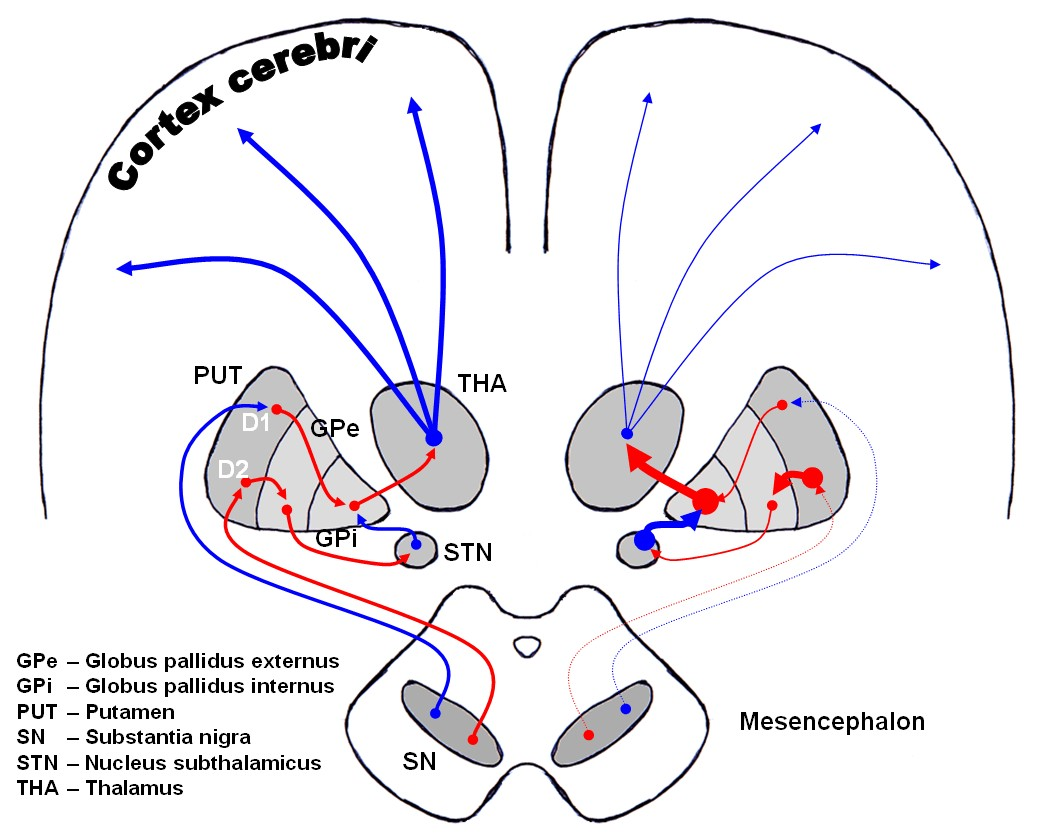
\includegraphics[width=0.5\linewidth]{FileAusiliari/Immagini/degenerative/dopamine-in-parkinsons-disease-illustration}
	\caption[Vie dopaminergiche]{L'immagine mostra le vie dopaminergiche del cervello umano in condizioni normali (a sinistra) e nella malattia di Parkinson (a destra). Le frecce rosse indicano la soppressione del bersaglio, quelle blu la stimolazione della struttura bersaglio. Caso per gentile concessione di Wikipedia, Radiopaedia.org, rID: 36286}
	\label{fig:dopamine-in-parkinsons-disease-illustration}
\end{figure*}

\subsection{Epidemiologia}
Il MP costituisce una delle principali cause di disabilità e mortalità nell'ambito delle patologie neurologiche, con una prevalenza particolarmente elevata negli Stati Uniti e in Canada (160-180 casi/100.000 abitanti). L'incidenza annuale in Nord America oscilla tra 108 e 212 casi ogni 100.000 individui di età $\geq$65 anni, con una prevalenza dello 0,3\% nella popolazione adulta $\geq$40 anni e dell'1,6\% nei soggetti ultrasessantacinquenni.
L'esordio della patologia mostra una significativa correlazione con l'età, manifestandosi tipicamente dalla quinta decade di vita, con un'età media alla diagnosi di 70,5 anni e una finestra di esordio prevalente tra i 45 e i 70 anni. Una variante giovanile può presentarsi tra i 20 e i 40 anni, sebbene l'esordio prima dei 30 anni risulti infrequente. La distribuzione per sesso evidenzia una predominanza maschile, particolarmente accentuata nella fascia d'età 50-60 anni.
L'eziologia del MP comprende fattori di rischio genetici, con particolare rilevanza nelle forme ad esordio precoce, e ambientali, tra cui l'esposizione a pesticidi e inquinanti atmosferici. Sono stati identificati fattori protettivi, inclusi il consumo di caffè, l'attività fisica e il fumo di sigaretta. La patologia si presenta prevalentemente in forma sporadica (85-90\% dei casi), mentre una minoranza dei casi (10-15\%) presenta familiarità positiva.

\subsubsection{Fattori di rischio}
L'eziopatogenesi del Morbo di Parkinson (MP) presenta una complessa interazione di fattori di rischio genetici, ambientali e non modificabili. L'anamnesi familiare positiva per MP in consanguinei di primo grado comporta un incremento del rischio relativo di 2-3 volte. Le forme monogeniche, rappresentanti meno del 10\% della casistica totale, manifestano pattern di ereditarietà autosomica dominante, recessiva o X-linked, caratterizzandosi per un esordio precoce rispetto alle forme sporadiche.
Le mutazioni eterozigoti del gene GBA1 costituiscono un significativo fattore di rischio genetico, unitamente ad alterazioni di altri geni codificanti per enzimi lisosomiali. Il coinvolgimento di geni quali SNCA, LRRK2, VPS35, Parkin, PINK1 e DJ-1 è stato ampiamente documentato. Particolare rilevanza assumono le mutazioni del gene Nurr1, determinante per l'identità neuronale dopaminergica, e del gene DJ-1, cruciale nella risposta allo stress ossidativo. Le alterazioni del gene PINK1, codificante per una chinasi mitocondriale, e del gene Park2, responsabile della sintesi della proteina parkina, sono associate a forme ad esordio precoce.
L'esposizione a neurotossine ambientali, inclusi mercurio, manganese, disolfuro di carbonio, solventi organici, MPTP e monossido di carbonio, può indurre degenerazione nigrostriatale e parkinsonismo. L'uso di neurolettici e l'abuso endovenoso di efedrone possono causare sindromi parkinsoniane potenzialmente irreversibili. Traumi cranici ripetuti, pesticidi, solventi e inquinamento atmosferico rappresentano ulteriori fattori di rischio ambientale documentati.
Tra i fattori non modificabili, l'età avanzata e il sesso maschile emergono come significativi predittori di rischio, con predominanza nella sesta decade di vita. Comorbidità quali depressione, ansia, stipsi, diabete mellito tipo 2, obesità e alterazioni del metabolismo del ferro sono state correlate a un incrementato rischio di MP.
Il consumo di tabacco e caffè, unitamente all'attività fisica regolare, ha mostrato effetti protettivi, sebbene di modesta entità. È fondamentale sottolineare che la maggioranza dei casi di MP rimane idiopatica, suggerendo un'eziologia multifattoriale.

\subsection{Presentazione  clinica}
La sintomatologia del Morbo di Parkinson manifesta un quadro clinico caratterizzato da manifestazioni motorie cardinali e sintomatologia non motoria associata. Il complesso sintomatologico motorio comprende tremore a riposo spesso asimmetrico con frequenza di 4-6 Hz, tipicamente descritto come "pill-rolling", bradicinesia manifestantesi con rallentamento motorio, ipomimia e ridotta oscillazione pendolare degli arti superiori durante la deambulazione, rigidità muscolare ("lead-pipe" o fenomeno della ruota dentata), e instabilità posturale documentabile attraverso il test della retropulsione. La deambulazione risulta caratterizzata da una progressione a piccoli passi con tendenza allo strascicamento e ridotta oscillazione degli arti superiori.
La sintomatologia accessoria include disartria con eloquio esplosivo secondario a incoordinazione linguo-diaframmatica, movimenti involontari della lingua con conseguente difficoltà protrusiva, e incremento della frequenza di ammiccamento palpebrale, quest'ultimo in contrasto con quanto osservato nella corea di Huntington. La disfunzione autonomica, i disturbi olfattivi, la sintomatologia algica, le alterazioni sensitive e i disturbi timici costituiscono il corredo sintomatologico non motorio. Il deterioramento cognitivo, con particolare coinvolgimento delle funzioni attentive, può manifestarsi e progredire nel decorso della patologia.
La progressione temporale della malattia evidenzia un esordio tipicamente unilaterale con successiva bilateralizzazione, manifestandosi prevalentemente nella sesta decade di vita. La responsività alla terapia dopaminergica, in particolare alla levodopa, rappresenta un elemento caratteristico, sebbene il tremore possa risultare farmacoresistente, in contrasto con la significativa risposta della bradicinesia e della rigidità. La variabilità fenotipica interindividuale costituisce un elemento distintivo della patologia.

\subsection{Approccio diagnostico}
L'iter diagnostico della malattia di Parkinson si fonda primariamente sulla valutazione clinica, data l'assenza di biomarcatori patognomonici. La diagnosi richiede la documentazione di bradicinesia associata ad almeno un sintomo cardine tra tremore a riposo o rigidità, valutati mediante la scala MDS-UPDRS standardizzata.
L'approccio diagnostico contempla un'accurata anamnesi ed esame obiettivo neurologico, focalizzati sull'identificazione dei sintomi cardinali: bradicinesia, tremore a riposo (4-6 Hz) tipicamente asimmetrico, rigidità e instabilità posturale. La responsività alla terapia dopaminergica, particolarmente evidente per bradicinesia e rigidità, costituisce un elemento diagnostico supportivo significativo, mentre una mancata risposta a dosaggi adeguati di levodopa suggerisce diagnosi alternative.
L'esclusione di parkinsonismi secondari richiede particolare attenzione all'insorgenza temporale dei sintomi e alla distribuzione topografica del coinvolgimento motorio. La diagnostica per immagini, sebbene non necessaria nelle presentazioni cliniche tipiche con adeguata risposta alla levodopa, può includere RM cerebrale, particolarmente utile mediante sequenze SWI per la valutazione del "swallow tail sign" nigrostriatale. La SPECT con 123I-FP-CIT (DaTscan) documenta la disfunzione dopaminergica presinaptica, mentre la PET con FDG consente la differenziazione metabolica tra PD e sindromi parkinsoniane atipiche.
L'analisi genetica, indicata in casi selezionati (esordio precoce, familiarità positiva, specifiche etnie), e la valutazione autonomica mediante scintigrafia miocardica con MIBG, che evidenzia la denervazione simpatica caratteristica, completano l'iter diagnostico. L'ecografia transcranica può evidenziare l'iperecogenicità della sostanza nera, supportando la diagnosi differenziale.
I criteri MDS stratificano la diagnosi in PD clinicamente stabilita e probabile, bilanciando specificità e sensibilità diagnostica nella pratica clinica.

\begin{Oss}
	La scala MDS-UPDRS (Movement Disorder Society-Unified Parkinson's Disease Rating Scale) è uno strumento di valutazione clinica ampiamente utilizzato per quantificare la gravità dei sintomi motori e non motori della malattia di Parkinson. Questa scala è stata sviluppata per migliorare la consistenza nella valutazione dei sintomi e per integrare meglio gli aspetti non motori della PD.
	Struttura: La scala MDS-UPDRS è composta da quattro sezioni:
	\begin{description}
		\item[Sezione I]{Esperienze non motorie della vita quotidiana. Questa sezione valuta aspetti come le capacità cognitive, i disturbi comportamentali e dell'umore}
		\item [Sezione II]{Esperienze motorie della vita quotidiana. Questa sezione valuta l'impatto dei sintomi motori sulle attività quotidiane}
		\item [Sezione III]{Esame motorio. Questa sezione valuta i segni motori della PD attraverso un esame clinico, come il tremore, la rigidità e la bradicinesia}
		\item[Sezione IV]{Complicanze della terapia. Questa sezione valuta le complicanze associate al trattamento farmacologico}
	\end{description}
	Il punteggio totale per le sezioni I-IV varia da 0 (nessuna disabilità) a 199 (disabilità totale). La sezione III, che valuta i sintomi motori, ha un punteggio che varia da 0 a 132.
	Oltre alla scala MDS-UPDRS, esistono altre scale di valutazione utilizzate nella PD, come la scala di Hoehn e Yahr e la scala di Schwab e England. La scala di Hoehn e Yahr valuta la gravità della malattia da 0 (nessuna malattia) a 5 (paziente costretto su sedia a rotelle o allettato senza assistenza).
\end{Oss}

\subsection{Anatomia patologica}
Dal punto di vista anatomopatologico il morbo di Parkinson si manifesta attraverso inclusioni proteiche intraneuronali denominate corpi di Lewy, costituiti primariamente da aggregati patologici di alfa-sinucleina, una proteina sinaptica fisiologicamente presente nel sistema nervoso centrale. L'accumulo di queste inclusioni, sebbene non patognomonico del morbo di Parkinson essendo documentabile anche nella demenza a corpi di Lewy, rappresenta una caratteristica istopatologica fondamentale quando localizzato nella substantia nigra, in associazione alla perdita neuronale dopaminergica. L'assenza di corpi di Lewy nelle forme post-encefalitiche, caratterizzate invece da grovigli neurofibrillari, e in alcune forme geneticamente determinate, sottolinea l'eterogeneità patogenetica della malattia.
La progressione spazio-temporale della patologia, codificata nello staging di Braak, delinea sei stadi evolutivi caratterizzati da una diffusione ascendente delle alterazioni neuropatologiche. Gli stadi iniziali (1-2) coinvolgono il nucleo motore dorsale dei nervi glossofaringeo e vago e il nucleo olfattivo anteriore, precedendo frequentemente la sintomatologia motoria. Gli stadi intermedi (3-4) documentano il coinvolgimento della substantia nigra pars compacta, del prosencefalo basale e della mesocorteccia temporale, correlando con l'esordio clinico della malattia. Gli stadi terminali (5-6) evidenziano una progressione neocorticale diffusa.
La patogenesi molecolare implica alterazioni del metabolismo dell'alfa-sinucleina, potenzialmente accelerate da disfunzioni delle proteine heat shock o dall'azione della dopamina. Il coinvolgimento della proteina parkin nella degradazione proteasomica evidenzia meccanismi neurodegenerativi potenzialmente indipendenti dalla formazione dei corpi di Lewy.
L'alfa-sinucleina, proteina fisiologicamente localizzata nelle terminazioni presinaptiche neuronali, manifesta nella patogenesi del morbo di Parkinson un processo patologico caratterizzato da misfolding proteico e successiva aggregazione in oligomeri, protofibrille e fibrille, culminante nella formazione dei corpi di Lewy intraneuronali. Questi aggregati proteici, considerati hallmark istopatologico della malattia, evidenziano particolare neurotossicità nella forma protofibrillare, determinando disfunzione e successiva degenerazione neuronale dopaminergica nigrostriatale.
L'identificazione di mutazioni nel gene SNCA, codificante per l'alfa-sinucleina, nelle forme familiari di malattia, unitamente alla documentazione di fenotipi clinici particolarmente aggressivi in presenza di duplicazione o triplicazione genica, ha fornito evidenze significative del ruolo causale di questa proteina nella patogenesi della malattia. La documentata capacità di trasmissione transcellulare dell'alfa-sinucleina patologica costituisce il substrato molecolare della progressione anatomopatologica descritta nello staging di Braak.
La disfunzione sinaptica correlata all'accumulo di alfa-sinucleina rappresenta un meccanismo patogenetico critico, modulato da fattori quali stress ossidativo, alterazioni del sistema ubiquitina-proteasoma e interazione con il metabolismo dopaminergico. Mutazioni nei geni parkin, PINK1 e DJ-1 influenzano il metabolismo dell'alfa-sinucleina attraverso alterazioni dei sistemi di degradazione proteica.
L'alfa-sinucleina costituisce attualmente un promettente target terapeutico, con particolare interesse per lo sviluppo di anticorpi monoclonali specifici e inibitori dell'aggregazione proteica, finalizzati al rallentamento della progressione patologica.

\subsection{Imaging}

\subsubsection{TC}
La TC manifesta un'utilità clinica circoscritta nella valutazione diagnostica primaria del MP, assumendo rilevanza nell'esclusione di patologie strutturali mimiche quali lesioni espansive, idrocefalo o alterazioni vascolari, particolarmente in presenza di presentazioni cliniche atipiche o "red flags" suggestive di diagnosi alternative.
Nel contesto della gestione terapeutica, la TC assume particolare rilevanza nella valutazione post-chirurgica della stimolazione cerebrale profonda (DBS), consentendo la verifica del corretto posizionamento degli elettrodi nel nucleo subtalamico (STN), tipicamente localizzati a 9mm dalla linea mediana, e l'identificazione di eventuali complicanze post-procedurali quali eventi emorragici, ischemici o fenomeni infiammatori transitori, questi ultimi caratterizzati da aree ipodense perilettrodiche a risoluzione graduale. L'utilità della metodica nel follow-up routinario post-DBS risulta secondaria.
La sensibilità subottimale della TC nella diagnosi differenziale tra PD e sindromi parkinsoniane atipiche, incluse atrofia multisistemica e paralisi sopranucleare progressiva, nonché nella distinzione dal tremore essenziale, ne limita significativamente l'applicazione clinica in questo contesto diagnostico.

\subsubsection{RM}
La RM è frequentemente normale nelle sequenze convenzionali (T1, T2, FLAIR) nelle fasi iniziali di malattia. L'implementazione di sequenze susceptibility-weighted imaging (SWI) o T2*-weighted ad alta risoluzione consente la visualizzazione del nigrosoma-1, struttura caratterizzata dal patognomonico "swallow tail sign", la cui perdita correla con la degenerazione dopaminergica nigrostriatale. L'accumulo patologico di ferro nella substantia nigra, quantificabile mediante sequenze SWI/T2* e incrementato del 50\% rispetto ai controlli, costituisce un ulteriore marker diagnostico, complementato dall'imaging della neuromelanina mediante sequenze T1 con impulsi di trasferimento di magnetizzazione (MTC).

\begin{figure*}[h]
	\centering
	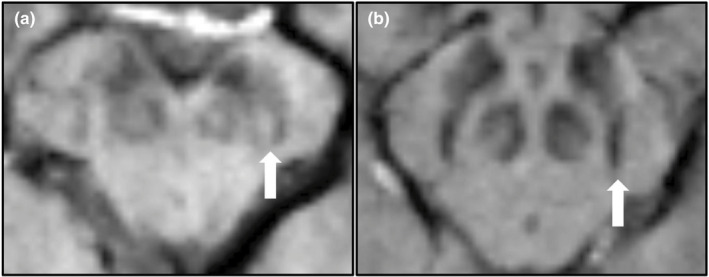
\includegraphics[width=0.8\linewidth]{FileAusiliari/Immagini/degenerative/BRB3-11-e02202-g002}
	\caption{Esempi di segno della coda di rondine (STS) in un individuo malato (a) e di STS assente in un individuo sano (b). Sono mostrate sezioni assiali del mesencefalo mappate tramite imaging pesato con suscettibilità (SWI). Le frecce bianche indicano la diversa configurazione del Nigrosoma-1 (N1). Da Brain Behav. 2021 May 24;11(7):e02202. doi: 10.1002/brb3.2202}
	\label{fig:brb3-11-e02202-g002}
\end{figure*}


La diagnosi differenziale delle sindromi parkinsoniane atipiche beneficia significativamente dell'imaging RM. L'atrofia multisistemica (MSA) evidenzia caratteristica atrofia putaminale, pontica e cerebellare, con ipointensità putaminale T2/SWI e "hot cross bun sign" pontino. La paralisi sopranucleare progressiva (PSP) manifesta atrofia mesencefalica con alterazione del rapporto mesencefalo-ponte, mentre la degenerazione corticobasale (CBD) presenta atrofia frontoparietale asimmetrica con iperintensità della sostanza bianca subcorticale.
Metodiche avanzate quali Diffusion Tensor Imaging (DTI) e risonanza magnetica funzionale (fMRI) consentono la caratterizzazione delle alterazioni microstrutturali della sostanza bianca e delle modificazioni funzionali cerebrali, sebbene la sensibilità nell'identificazione della progressione patologica e nella valutazione della risposta terapeutica necessiti ulteriore validazione. Le limitazioni metodologiche includono variabilità interindividuale e sovrapposizione dei reperti radiologici nelle diverse sindromi parkinsoniane.

\subsection{Trattamento e prognosi}

\subsection{Checklist di refertazione}

\begin{itemize}[label=$\square$] % Riquadro vuoto come simbolo
	\item Escludi altre cause di parkinsonismo (es ictus)
	\item Controlla il segnale dei nigrosomi
	\item Controlla il trofismo delle strutture sottotentoriali
\end{itemize}

\subsection{Bibliografia}
\small{
	
	
}

\note{Nota a margine}
\expl{Nota a margine colorata}
\input{Capitoli/vascolare/stroke_ischemico.tex}
\input{Capitoli/vascolare/patologia_vascolare.tex}
\input{Capitoli/vascolare/malattia_piccoli_vasi.tex}
\input{Capitoli/vascolare/emorragie_intraparenchimali.tex}
\input{Capitoli/vascolare/emorragia_subaracnoidea.tex}
\input{Capitoli/vascolare/trombosi_venosa.tex}
\input{Capitoli/degenerative/approccio.tex}
\input{Capitoli/degenerative/degenerative.tex}
\section{Morbo di Parkinson}

\subsection{Definizione}

\subsection{Eziologia}

\begin{figure*}[h]
	\centering
	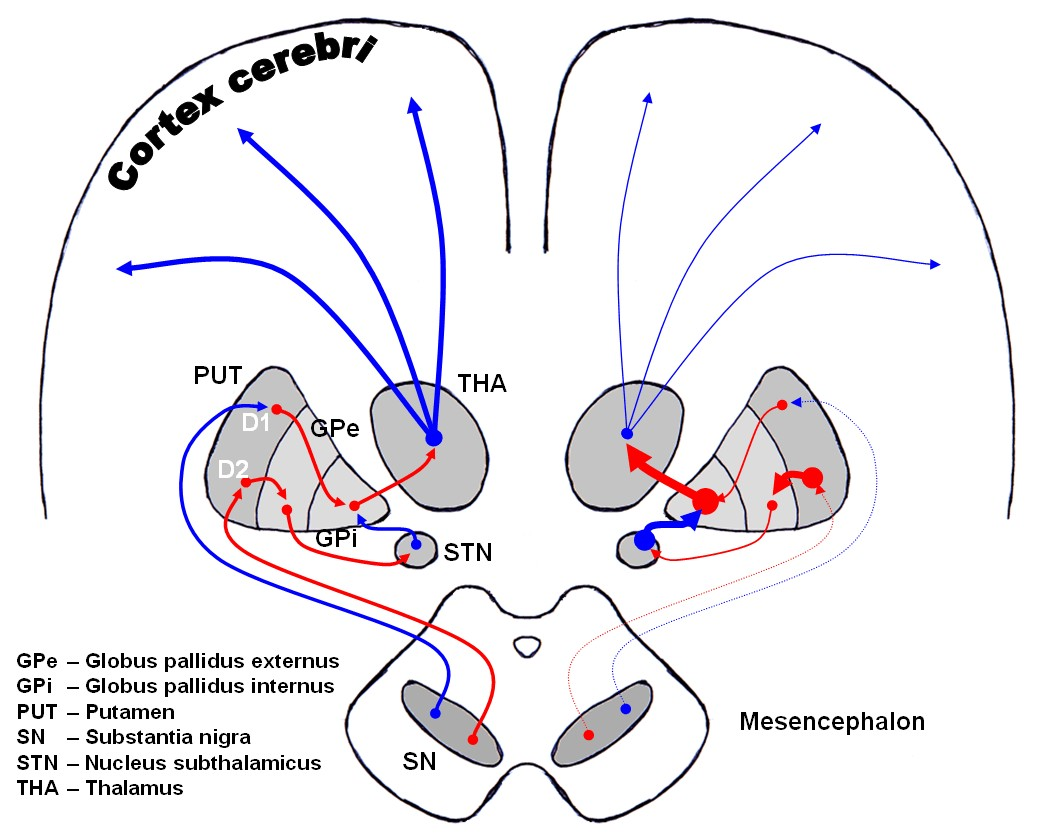
\includegraphics[width=0.5\linewidth]{FileAusiliari/Immagini/degenerative/dopamine-in-parkinsons-disease-illustration}
	\caption[Vie dopaminergiche]{L'immagine mostra le vie dopaminergiche del cervello umano in condizioni normali (a sinistra) e nella malattia di Parkinson (a destra). Le frecce rosse indicano la soppressione del bersaglio, quelle blu la stimolazione della struttura bersaglio. Caso per gentile concessione di Wikipedia, Radiopaedia.org, rID: 36286}
	\label{fig:dopamine-in-parkinsons-disease-illustration}
\end{figure*}

\subsection{Epidemiologia}
Il MP costituisce una delle principali cause di disabilità e mortalità nell'ambito delle patologie neurologiche, con una prevalenza particolarmente elevata negli Stati Uniti e in Canada (160-180 casi/100.000 abitanti). L'incidenza annuale in Nord America oscilla tra 108 e 212 casi ogni 100.000 individui di età $\geq$65 anni, con una prevalenza dello 0,3\% nella popolazione adulta $\geq$40 anni e dell'1,6\% nei soggetti ultrasessantacinquenni.
L'esordio della patologia mostra una significativa correlazione con l'età, manifestandosi tipicamente dalla quinta decade di vita, con un'età media alla diagnosi di 70,5 anni e una finestra di esordio prevalente tra i 45 e i 70 anni. Una variante giovanile può presentarsi tra i 20 e i 40 anni, sebbene l'esordio prima dei 30 anni risulti infrequente. La distribuzione per sesso evidenzia una predominanza maschile, particolarmente accentuata nella fascia d'età 50-60 anni.
L'eziologia del MP comprende fattori di rischio genetici, con particolare rilevanza nelle forme ad esordio precoce, e ambientali, tra cui l'esposizione a pesticidi e inquinanti atmosferici. Sono stati identificati fattori protettivi, inclusi il consumo di caffè, l'attività fisica e il fumo di sigaretta. La patologia si presenta prevalentemente in forma sporadica (85-90\% dei casi), mentre una minoranza dei casi (10-15\%) presenta familiarità positiva.

\subsubsection{Fattori di rischio}
L'eziopatogenesi del Morbo di Parkinson (MP) presenta una complessa interazione di fattori di rischio genetici, ambientali e non modificabili. L'anamnesi familiare positiva per MP in consanguinei di primo grado comporta un incremento del rischio relativo di 2-3 volte. Le forme monogeniche, rappresentanti meno del 10\% della casistica totale, manifestano pattern di ereditarietà autosomica dominante, recessiva o X-linked, caratterizzandosi per un esordio precoce rispetto alle forme sporadiche.
Le mutazioni eterozigoti del gene GBA1 costituiscono un significativo fattore di rischio genetico, unitamente ad alterazioni di altri geni codificanti per enzimi lisosomiali. Il coinvolgimento di geni quali SNCA, LRRK2, VPS35, Parkin, PINK1 e DJ-1 è stato ampiamente documentato. Particolare rilevanza assumono le mutazioni del gene Nurr1, determinante per l'identità neuronale dopaminergica, e del gene DJ-1, cruciale nella risposta allo stress ossidativo. Le alterazioni del gene PINK1, codificante per una chinasi mitocondriale, e del gene Park2, responsabile della sintesi della proteina parkina, sono associate a forme ad esordio precoce.
L'esposizione a neurotossine ambientali, inclusi mercurio, manganese, disolfuro di carbonio, solventi organici, MPTP e monossido di carbonio, può indurre degenerazione nigrostriatale e parkinsonismo. L'uso di neurolettici e l'abuso endovenoso di efedrone possono causare sindromi parkinsoniane potenzialmente irreversibili. Traumi cranici ripetuti, pesticidi, solventi e inquinamento atmosferico rappresentano ulteriori fattori di rischio ambientale documentati.
Tra i fattori non modificabili, l'età avanzata e il sesso maschile emergono come significativi predittori di rischio, con predominanza nella sesta decade di vita. Comorbidità quali depressione, ansia, stipsi, diabete mellito tipo 2, obesità e alterazioni del metabolismo del ferro sono state correlate a un incrementato rischio di MP.
Il consumo di tabacco e caffè, unitamente all'attività fisica regolare, ha mostrato effetti protettivi, sebbene di modesta entità. È fondamentale sottolineare che la maggioranza dei casi di MP rimane idiopatica, suggerendo un'eziologia multifattoriale.

\subsection{Presentazione  clinica}
La sintomatologia del Morbo di Parkinson manifesta un quadro clinico caratterizzato da manifestazioni motorie cardinali e sintomatologia non motoria associata. Il complesso sintomatologico motorio comprende tremore a riposo spesso asimmetrico con frequenza di 4-6 Hz, tipicamente descritto come "pill-rolling", bradicinesia manifestantesi con rallentamento motorio, ipomimia e ridotta oscillazione pendolare degli arti superiori durante la deambulazione, rigidità muscolare ("lead-pipe" o fenomeno della ruota dentata), e instabilità posturale documentabile attraverso il test della retropulsione. La deambulazione risulta caratterizzata da una progressione a piccoli passi con tendenza allo strascicamento e ridotta oscillazione degli arti superiori.
La sintomatologia accessoria include disartria con eloquio esplosivo secondario a incoordinazione linguo-diaframmatica, movimenti involontari della lingua con conseguente difficoltà protrusiva, e incremento della frequenza di ammiccamento palpebrale, quest'ultimo in contrasto con quanto osservato nella corea di Huntington. La disfunzione autonomica, i disturbi olfattivi, la sintomatologia algica, le alterazioni sensitive e i disturbi timici costituiscono il corredo sintomatologico non motorio. Il deterioramento cognitivo, con particolare coinvolgimento delle funzioni attentive, può manifestarsi e progredire nel decorso della patologia.
La progressione temporale della malattia evidenzia un esordio tipicamente unilaterale con successiva bilateralizzazione, manifestandosi prevalentemente nella sesta decade di vita. La responsività alla terapia dopaminergica, in particolare alla levodopa, rappresenta un elemento caratteristico, sebbene il tremore possa risultare farmacoresistente, in contrasto con la significativa risposta della bradicinesia e della rigidità. La variabilità fenotipica interindividuale costituisce un elemento distintivo della patologia.

\subsection{Approccio diagnostico}
L'iter diagnostico della malattia di Parkinson si fonda primariamente sulla valutazione clinica, data l'assenza di biomarcatori patognomonici. La diagnosi richiede la documentazione di bradicinesia associata ad almeno un sintomo cardine tra tremore a riposo o rigidità, valutati mediante la scala MDS-UPDRS standardizzata.
L'approccio diagnostico contempla un'accurata anamnesi ed esame obiettivo neurologico, focalizzati sull'identificazione dei sintomi cardinali: bradicinesia, tremore a riposo (4-6 Hz) tipicamente asimmetrico, rigidità e instabilità posturale. La responsività alla terapia dopaminergica, particolarmente evidente per bradicinesia e rigidità, costituisce un elemento diagnostico supportivo significativo, mentre una mancata risposta a dosaggi adeguati di levodopa suggerisce diagnosi alternative.
L'esclusione di parkinsonismi secondari richiede particolare attenzione all'insorgenza temporale dei sintomi e alla distribuzione topografica del coinvolgimento motorio. La diagnostica per immagini, sebbene non necessaria nelle presentazioni cliniche tipiche con adeguata risposta alla levodopa, può includere RM cerebrale, particolarmente utile mediante sequenze SWI per la valutazione del "swallow tail sign" nigrostriatale. La SPECT con 123I-FP-CIT (DaTscan) documenta la disfunzione dopaminergica presinaptica, mentre la PET con FDG consente la differenziazione metabolica tra PD e sindromi parkinsoniane atipiche.
L'analisi genetica, indicata in casi selezionati (esordio precoce, familiarità positiva, specifiche etnie), e la valutazione autonomica mediante scintigrafia miocardica con MIBG, che evidenzia la denervazione simpatica caratteristica, completano l'iter diagnostico. L'ecografia transcranica può evidenziare l'iperecogenicità della sostanza nera, supportando la diagnosi differenziale.
I criteri MDS stratificano la diagnosi in PD clinicamente stabilita e probabile, bilanciando specificità e sensibilità diagnostica nella pratica clinica.

\begin{Oss}
	La scala MDS-UPDRS (Movement Disorder Society-Unified Parkinson's Disease Rating Scale) è uno strumento di valutazione clinica ampiamente utilizzato per quantificare la gravità dei sintomi motori e non motori della malattia di Parkinson. Questa scala è stata sviluppata per migliorare la consistenza nella valutazione dei sintomi e per integrare meglio gli aspetti non motori della PD.
	Struttura: La scala MDS-UPDRS è composta da quattro sezioni:
	\begin{description}
		\item[Sezione I]{Esperienze non motorie della vita quotidiana. Questa sezione valuta aspetti come le capacità cognitive, i disturbi comportamentali e dell'umore}
		\item [Sezione II]{Esperienze motorie della vita quotidiana. Questa sezione valuta l'impatto dei sintomi motori sulle attività quotidiane}
		\item [Sezione III]{Esame motorio. Questa sezione valuta i segni motori della PD attraverso un esame clinico, come il tremore, la rigidità e la bradicinesia}
		\item[Sezione IV]{Complicanze della terapia. Questa sezione valuta le complicanze associate al trattamento farmacologico}
	\end{description}
	Il punteggio totale per le sezioni I-IV varia da 0 (nessuna disabilità) a 199 (disabilità totale). La sezione III, che valuta i sintomi motori, ha un punteggio che varia da 0 a 132.
	Oltre alla scala MDS-UPDRS, esistono altre scale di valutazione utilizzate nella PD, come la scala di Hoehn e Yahr e la scala di Schwab e England. La scala di Hoehn e Yahr valuta la gravità della malattia da 0 (nessuna malattia) a 5 (paziente costretto su sedia a rotelle o allettato senza assistenza).
\end{Oss}

\subsection{Anatomia patologica}
Dal punto di vista anatomopatologico il morbo di Parkinson si manifesta attraverso inclusioni proteiche intraneuronali denominate corpi di Lewy, costituiti primariamente da aggregati patologici di alfa-sinucleina, una proteina sinaptica fisiologicamente presente nel sistema nervoso centrale. L'accumulo di queste inclusioni, sebbene non patognomonico del morbo di Parkinson essendo documentabile anche nella demenza a corpi di Lewy, rappresenta una caratteristica istopatologica fondamentale quando localizzato nella substantia nigra, in associazione alla perdita neuronale dopaminergica. L'assenza di corpi di Lewy nelle forme post-encefalitiche, caratterizzate invece da grovigli neurofibrillari, e in alcune forme geneticamente determinate, sottolinea l'eterogeneità patogenetica della malattia.
La progressione spazio-temporale della patologia, codificata nello staging di Braak, delinea sei stadi evolutivi caratterizzati da una diffusione ascendente delle alterazioni neuropatologiche. Gli stadi iniziali (1-2) coinvolgono il nucleo motore dorsale dei nervi glossofaringeo e vago e il nucleo olfattivo anteriore, precedendo frequentemente la sintomatologia motoria. Gli stadi intermedi (3-4) documentano il coinvolgimento della substantia nigra pars compacta, del prosencefalo basale e della mesocorteccia temporale, correlando con l'esordio clinico della malattia. Gli stadi terminali (5-6) evidenziano una progressione neocorticale diffusa.
La patogenesi molecolare implica alterazioni del metabolismo dell'alfa-sinucleina, potenzialmente accelerate da disfunzioni delle proteine heat shock o dall'azione della dopamina. Il coinvolgimento della proteina parkin nella degradazione proteasomica evidenzia meccanismi neurodegenerativi potenzialmente indipendenti dalla formazione dei corpi di Lewy.
L'alfa-sinucleina, proteina fisiologicamente localizzata nelle terminazioni presinaptiche neuronali, manifesta nella patogenesi del morbo di Parkinson un processo patologico caratterizzato da misfolding proteico e successiva aggregazione in oligomeri, protofibrille e fibrille, culminante nella formazione dei corpi di Lewy intraneuronali. Questi aggregati proteici, considerati hallmark istopatologico della malattia, evidenziano particolare neurotossicità nella forma protofibrillare, determinando disfunzione e successiva degenerazione neuronale dopaminergica nigrostriatale.
L'identificazione di mutazioni nel gene SNCA, codificante per l'alfa-sinucleina, nelle forme familiari di malattia, unitamente alla documentazione di fenotipi clinici particolarmente aggressivi in presenza di duplicazione o triplicazione genica, ha fornito evidenze significative del ruolo causale di questa proteina nella patogenesi della malattia. La documentata capacità di trasmissione transcellulare dell'alfa-sinucleina patologica costituisce il substrato molecolare della progressione anatomopatologica descritta nello staging di Braak.
La disfunzione sinaptica correlata all'accumulo di alfa-sinucleina rappresenta un meccanismo patogenetico critico, modulato da fattori quali stress ossidativo, alterazioni del sistema ubiquitina-proteasoma e interazione con il metabolismo dopaminergico. Mutazioni nei geni parkin, PINK1 e DJ-1 influenzano il metabolismo dell'alfa-sinucleina attraverso alterazioni dei sistemi di degradazione proteica.
L'alfa-sinucleina costituisce attualmente un promettente target terapeutico, con particolare interesse per lo sviluppo di anticorpi monoclonali specifici e inibitori dell'aggregazione proteica, finalizzati al rallentamento della progressione patologica.

\subsection{Imaging}

\subsubsection{TC}
La TC manifesta un'utilità clinica circoscritta nella valutazione diagnostica primaria del MP, assumendo rilevanza nell'esclusione di patologie strutturali mimiche quali lesioni espansive, idrocefalo o alterazioni vascolari, particolarmente in presenza di presentazioni cliniche atipiche o "red flags" suggestive di diagnosi alternative.
Nel contesto della gestione terapeutica, la TC assume particolare rilevanza nella valutazione post-chirurgica della stimolazione cerebrale profonda (DBS), consentendo la verifica del corretto posizionamento degli elettrodi nel nucleo subtalamico (STN), tipicamente localizzati a 9mm dalla linea mediana, e l'identificazione di eventuali complicanze post-procedurali quali eventi emorragici, ischemici o fenomeni infiammatori transitori, questi ultimi caratterizzati da aree ipodense perilettrodiche a risoluzione graduale. L'utilità della metodica nel follow-up routinario post-DBS risulta secondaria.
La sensibilità subottimale della TC nella diagnosi differenziale tra PD e sindromi parkinsoniane atipiche, incluse atrofia multisistemica e paralisi sopranucleare progressiva, nonché nella distinzione dal tremore essenziale, ne limita significativamente l'applicazione clinica in questo contesto diagnostico.

\subsubsection{RM}
La RM è frequentemente normale nelle sequenze convenzionali (T1, T2, FLAIR) nelle fasi iniziali di malattia. L'implementazione di sequenze susceptibility-weighted imaging (SWI) o T2*-weighted ad alta risoluzione consente la visualizzazione del nigrosoma-1, struttura caratterizzata dal patognomonico "swallow tail sign", la cui perdita correla con la degenerazione dopaminergica nigrostriatale. L'accumulo patologico di ferro nella substantia nigra, quantificabile mediante sequenze SWI/T2* e incrementato del 50\% rispetto ai controlli, costituisce un ulteriore marker diagnostico, complementato dall'imaging della neuromelanina mediante sequenze T1 con impulsi di trasferimento di magnetizzazione (MTC).

\begin{figure*}[h]
	\centering
	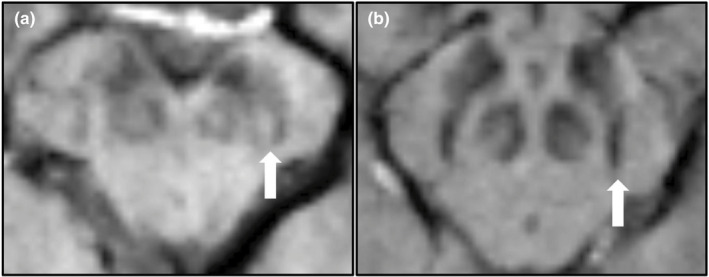
\includegraphics[width=0.8\linewidth]{FileAusiliari/Immagini/degenerative/BRB3-11-e02202-g002}
	\caption{Esempi di segno della coda di rondine (STS) in un individuo malato (a) e di STS assente in un individuo sano (b). Sono mostrate sezioni assiali del mesencefalo mappate tramite imaging pesato con suscettibilità (SWI). Le frecce bianche indicano la diversa configurazione del Nigrosoma-1 (N1). Da Brain Behav. 2021 May 24;11(7):e02202. doi: 10.1002/brb3.2202}
	\label{fig:brb3-11-e02202-g002}
\end{figure*}


La diagnosi differenziale delle sindromi parkinsoniane atipiche beneficia significativamente dell'imaging RM. L'atrofia multisistemica (MSA) evidenzia caratteristica atrofia putaminale, pontica e cerebellare, con ipointensità putaminale T2/SWI e "hot cross bun sign" pontino. La paralisi sopranucleare progressiva (PSP) manifesta atrofia mesencefalica con alterazione del rapporto mesencefalo-ponte, mentre la degenerazione corticobasale (CBD) presenta atrofia frontoparietale asimmetrica con iperintensità della sostanza bianca subcorticale.
Metodiche avanzate quali Diffusion Tensor Imaging (DTI) e risonanza magnetica funzionale (fMRI) consentono la caratterizzazione delle alterazioni microstrutturali della sostanza bianca e delle modificazioni funzionali cerebrali, sebbene la sensibilità nell'identificazione della progressione patologica e nella valutazione della risposta terapeutica necessiti ulteriore validazione. Le limitazioni metodologiche includono variabilità interindividuale e sovrapposizione dei reperti radiologici nelle diverse sindromi parkinsoniane.

\subsection{Trattamento e prognosi}

\subsection{Checklist di refertazione}

\begin{itemize}[label=$\square$] % Riquadro vuoto come simbolo
	\item Escludi altre cause di parkinsonismo (es ictus)
	\item Controlla il segnale dei nigrosomi
	\item Controlla il trofismo delle strutture sottotentoriali
\end{itemize}

\subsection{Bibliografia}
\small{
	
	
}

\note{Nota a margine}
\expl{Nota a margine colorata}
\input{Capitoli/degenerative/approccio.tex}
\input{Capitoli/degenerative/degenerative.tex}
\section{Morbo di Parkinson}

\subsection{Definizione}

\subsection{Eziologia}

\begin{figure*}[h]
	\centering
	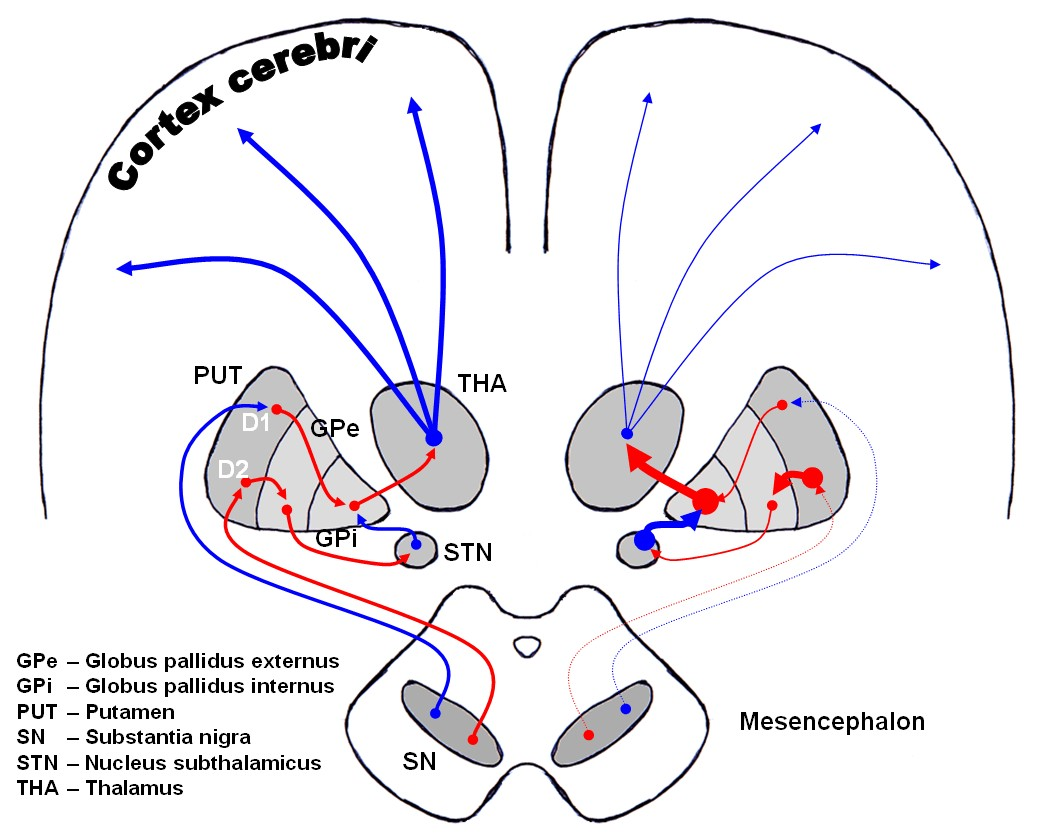
\includegraphics[width=0.5\linewidth]{FileAusiliari/Immagini/degenerative/dopamine-in-parkinsons-disease-illustration}
	\caption[Vie dopaminergiche]{L'immagine mostra le vie dopaminergiche del cervello umano in condizioni normali (a sinistra) e nella malattia di Parkinson (a destra). Le frecce rosse indicano la soppressione del bersaglio, quelle blu la stimolazione della struttura bersaglio. Caso per gentile concessione di Wikipedia, Radiopaedia.org, rID: 36286}
	\label{fig:dopamine-in-parkinsons-disease-illustration}
\end{figure*}

\subsection{Epidemiologia}
Il MP costituisce una delle principali cause di disabilità e mortalità nell'ambito delle patologie neurologiche, con una prevalenza particolarmente elevata negli Stati Uniti e in Canada (160-180 casi/100.000 abitanti). L'incidenza annuale in Nord America oscilla tra 108 e 212 casi ogni 100.000 individui di età $\geq$65 anni, con una prevalenza dello 0,3\% nella popolazione adulta $\geq$40 anni e dell'1,6\% nei soggetti ultrasessantacinquenni.
L'esordio della patologia mostra una significativa correlazione con l'età, manifestandosi tipicamente dalla quinta decade di vita, con un'età media alla diagnosi di 70,5 anni e una finestra di esordio prevalente tra i 45 e i 70 anni. Una variante giovanile può presentarsi tra i 20 e i 40 anni, sebbene l'esordio prima dei 30 anni risulti infrequente. La distribuzione per sesso evidenzia una predominanza maschile, particolarmente accentuata nella fascia d'età 50-60 anni.
L'eziologia del MP comprende fattori di rischio genetici, con particolare rilevanza nelle forme ad esordio precoce, e ambientali, tra cui l'esposizione a pesticidi e inquinanti atmosferici. Sono stati identificati fattori protettivi, inclusi il consumo di caffè, l'attività fisica e il fumo di sigaretta. La patologia si presenta prevalentemente in forma sporadica (85-90\% dei casi), mentre una minoranza dei casi (10-15\%) presenta familiarità positiva.

\subsubsection{Fattori di rischio}
L'eziopatogenesi del Morbo di Parkinson (MP) presenta una complessa interazione di fattori di rischio genetici, ambientali e non modificabili. L'anamnesi familiare positiva per MP in consanguinei di primo grado comporta un incremento del rischio relativo di 2-3 volte. Le forme monogeniche, rappresentanti meno del 10\% della casistica totale, manifestano pattern di ereditarietà autosomica dominante, recessiva o X-linked, caratterizzandosi per un esordio precoce rispetto alle forme sporadiche.
Le mutazioni eterozigoti del gene GBA1 costituiscono un significativo fattore di rischio genetico, unitamente ad alterazioni di altri geni codificanti per enzimi lisosomiali. Il coinvolgimento di geni quali SNCA, LRRK2, VPS35, Parkin, PINK1 e DJ-1 è stato ampiamente documentato. Particolare rilevanza assumono le mutazioni del gene Nurr1, determinante per l'identità neuronale dopaminergica, e del gene DJ-1, cruciale nella risposta allo stress ossidativo. Le alterazioni del gene PINK1, codificante per una chinasi mitocondriale, e del gene Park2, responsabile della sintesi della proteina parkina, sono associate a forme ad esordio precoce.
L'esposizione a neurotossine ambientali, inclusi mercurio, manganese, disolfuro di carbonio, solventi organici, MPTP e monossido di carbonio, può indurre degenerazione nigrostriatale e parkinsonismo. L'uso di neurolettici e l'abuso endovenoso di efedrone possono causare sindromi parkinsoniane potenzialmente irreversibili. Traumi cranici ripetuti, pesticidi, solventi e inquinamento atmosferico rappresentano ulteriori fattori di rischio ambientale documentati.
Tra i fattori non modificabili, l'età avanzata e il sesso maschile emergono come significativi predittori di rischio, con predominanza nella sesta decade di vita. Comorbidità quali depressione, ansia, stipsi, diabete mellito tipo 2, obesità e alterazioni del metabolismo del ferro sono state correlate a un incrementato rischio di MP.
Il consumo di tabacco e caffè, unitamente all'attività fisica regolare, ha mostrato effetti protettivi, sebbene di modesta entità. È fondamentale sottolineare che la maggioranza dei casi di MP rimane idiopatica, suggerendo un'eziologia multifattoriale.

\subsection{Presentazione  clinica}
La sintomatologia del Morbo di Parkinson manifesta un quadro clinico caratterizzato da manifestazioni motorie cardinali e sintomatologia non motoria associata. Il complesso sintomatologico motorio comprende tremore a riposo spesso asimmetrico con frequenza di 4-6 Hz, tipicamente descritto come "pill-rolling", bradicinesia manifestantesi con rallentamento motorio, ipomimia e ridotta oscillazione pendolare degli arti superiori durante la deambulazione, rigidità muscolare ("lead-pipe" o fenomeno della ruota dentata), e instabilità posturale documentabile attraverso il test della retropulsione. La deambulazione risulta caratterizzata da una progressione a piccoli passi con tendenza allo strascicamento e ridotta oscillazione degli arti superiori.
La sintomatologia accessoria include disartria con eloquio esplosivo secondario a incoordinazione linguo-diaframmatica, movimenti involontari della lingua con conseguente difficoltà protrusiva, e incremento della frequenza di ammiccamento palpebrale, quest'ultimo in contrasto con quanto osservato nella corea di Huntington. La disfunzione autonomica, i disturbi olfattivi, la sintomatologia algica, le alterazioni sensitive e i disturbi timici costituiscono il corredo sintomatologico non motorio. Il deterioramento cognitivo, con particolare coinvolgimento delle funzioni attentive, può manifestarsi e progredire nel decorso della patologia.
La progressione temporale della malattia evidenzia un esordio tipicamente unilaterale con successiva bilateralizzazione, manifestandosi prevalentemente nella sesta decade di vita. La responsività alla terapia dopaminergica, in particolare alla levodopa, rappresenta un elemento caratteristico, sebbene il tremore possa risultare farmacoresistente, in contrasto con la significativa risposta della bradicinesia e della rigidità. La variabilità fenotipica interindividuale costituisce un elemento distintivo della patologia.

\subsection{Approccio diagnostico}
L'iter diagnostico della malattia di Parkinson si fonda primariamente sulla valutazione clinica, data l'assenza di biomarcatori patognomonici. La diagnosi richiede la documentazione di bradicinesia associata ad almeno un sintomo cardine tra tremore a riposo o rigidità, valutati mediante la scala MDS-UPDRS standardizzata.
L'approccio diagnostico contempla un'accurata anamnesi ed esame obiettivo neurologico, focalizzati sull'identificazione dei sintomi cardinali: bradicinesia, tremore a riposo (4-6 Hz) tipicamente asimmetrico, rigidità e instabilità posturale. La responsività alla terapia dopaminergica, particolarmente evidente per bradicinesia e rigidità, costituisce un elemento diagnostico supportivo significativo, mentre una mancata risposta a dosaggi adeguati di levodopa suggerisce diagnosi alternative.
L'esclusione di parkinsonismi secondari richiede particolare attenzione all'insorgenza temporale dei sintomi e alla distribuzione topografica del coinvolgimento motorio. La diagnostica per immagini, sebbene non necessaria nelle presentazioni cliniche tipiche con adeguata risposta alla levodopa, può includere RM cerebrale, particolarmente utile mediante sequenze SWI per la valutazione del "swallow tail sign" nigrostriatale. La SPECT con 123I-FP-CIT (DaTscan) documenta la disfunzione dopaminergica presinaptica, mentre la PET con FDG consente la differenziazione metabolica tra PD e sindromi parkinsoniane atipiche.
L'analisi genetica, indicata in casi selezionati (esordio precoce, familiarità positiva, specifiche etnie), e la valutazione autonomica mediante scintigrafia miocardica con MIBG, che evidenzia la denervazione simpatica caratteristica, completano l'iter diagnostico. L'ecografia transcranica può evidenziare l'iperecogenicità della sostanza nera, supportando la diagnosi differenziale.
I criteri MDS stratificano la diagnosi in PD clinicamente stabilita e probabile, bilanciando specificità e sensibilità diagnostica nella pratica clinica.

\begin{Oss}
	La scala MDS-UPDRS (Movement Disorder Society-Unified Parkinson's Disease Rating Scale) è uno strumento di valutazione clinica ampiamente utilizzato per quantificare la gravità dei sintomi motori e non motori della malattia di Parkinson. Questa scala è stata sviluppata per migliorare la consistenza nella valutazione dei sintomi e per integrare meglio gli aspetti non motori della PD.
	Struttura: La scala MDS-UPDRS è composta da quattro sezioni:
	\begin{description}
		\item[Sezione I]{Esperienze non motorie della vita quotidiana. Questa sezione valuta aspetti come le capacità cognitive, i disturbi comportamentali e dell'umore}
		\item [Sezione II]{Esperienze motorie della vita quotidiana. Questa sezione valuta l'impatto dei sintomi motori sulle attività quotidiane}
		\item [Sezione III]{Esame motorio. Questa sezione valuta i segni motori della PD attraverso un esame clinico, come il tremore, la rigidità e la bradicinesia}
		\item[Sezione IV]{Complicanze della terapia. Questa sezione valuta le complicanze associate al trattamento farmacologico}
	\end{description}
	Il punteggio totale per le sezioni I-IV varia da 0 (nessuna disabilità) a 199 (disabilità totale). La sezione III, che valuta i sintomi motori, ha un punteggio che varia da 0 a 132.
	Oltre alla scala MDS-UPDRS, esistono altre scale di valutazione utilizzate nella PD, come la scala di Hoehn e Yahr e la scala di Schwab e England. La scala di Hoehn e Yahr valuta la gravità della malattia da 0 (nessuna malattia) a 5 (paziente costretto su sedia a rotelle o allettato senza assistenza).
\end{Oss}

\subsection{Anatomia patologica}
Dal punto di vista anatomopatologico il morbo di Parkinson si manifesta attraverso inclusioni proteiche intraneuronali denominate corpi di Lewy, costituiti primariamente da aggregati patologici di alfa-sinucleina, una proteina sinaptica fisiologicamente presente nel sistema nervoso centrale. L'accumulo di queste inclusioni, sebbene non patognomonico del morbo di Parkinson essendo documentabile anche nella demenza a corpi di Lewy, rappresenta una caratteristica istopatologica fondamentale quando localizzato nella substantia nigra, in associazione alla perdita neuronale dopaminergica. L'assenza di corpi di Lewy nelle forme post-encefalitiche, caratterizzate invece da grovigli neurofibrillari, e in alcune forme geneticamente determinate, sottolinea l'eterogeneità patogenetica della malattia.
La progressione spazio-temporale della patologia, codificata nello staging di Braak, delinea sei stadi evolutivi caratterizzati da una diffusione ascendente delle alterazioni neuropatologiche. Gli stadi iniziali (1-2) coinvolgono il nucleo motore dorsale dei nervi glossofaringeo e vago e il nucleo olfattivo anteriore, precedendo frequentemente la sintomatologia motoria. Gli stadi intermedi (3-4) documentano il coinvolgimento della substantia nigra pars compacta, del prosencefalo basale e della mesocorteccia temporale, correlando con l'esordio clinico della malattia. Gli stadi terminali (5-6) evidenziano una progressione neocorticale diffusa.
La patogenesi molecolare implica alterazioni del metabolismo dell'alfa-sinucleina, potenzialmente accelerate da disfunzioni delle proteine heat shock o dall'azione della dopamina. Il coinvolgimento della proteina parkin nella degradazione proteasomica evidenzia meccanismi neurodegenerativi potenzialmente indipendenti dalla formazione dei corpi di Lewy.
L'alfa-sinucleina, proteina fisiologicamente localizzata nelle terminazioni presinaptiche neuronali, manifesta nella patogenesi del morbo di Parkinson un processo patologico caratterizzato da misfolding proteico e successiva aggregazione in oligomeri, protofibrille e fibrille, culminante nella formazione dei corpi di Lewy intraneuronali. Questi aggregati proteici, considerati hallmark istopatologico della malattia, evidenziano particolare neurotossicità nella forma protofibrillare, determinando disfunzione e successiva degenerazione neuronale dopaminergica nigrostriatale.
L'identificazione di mutazioni nel gene SNCA, codificante per l'alfa-sinucleina, nelle forme familiari di malattia, unitamente alla documentazione di fenotipi clinici particolarmente aggressivi in presenza di duplicazione o triplicazione genica, ha fornito evidenze significative del ruolo causale di questa proteina nella patogenesi della malattia. La documentata capacità di trasmissione transcellulare dell'alfa-sinucleina patologica costituisce il substrato molecolare della progressione anatomopatologica descritta nello staging di Braak.
La disfunzione sinaptica correlata all'accumulo di alfa-sinucleina rappresenta un meccanismo patogenetico critico, modulato da fattori quali stress ossidativo, alterazioni del sistema ubiquitina-proteasoma e interazione con il metabolismo dopaminergico. Mutazioni nei geni parkin, PINK1 e DJ-1 influenzano il metabolismo dell'alfa-sinucleina attraverso alterazioni dei sistemi di degradazione proteica.
L'alfa-sinucleina costituisce attualmente un promettente target terapeutico, con particolare interesse per lo sviluppo di anticorpi monoclonali specifici e inibitori dell'aggregazione proteica, finalizzati al rallentamento della progressione patologica.

\subsection{Imaging}

\subsubsection{TC}
La TC manifesta un'utilità clinica circoscritta nella valutazione diagnostica primaria del MP, assumendo rilevanza nell'esclusione di patologie strutturali mimiche quali lesioni espansive, idrocefalo o alterazioni vascolari, particolarmente in presenza di presentazioni cliniche atipiche o "red flags" suggestive di diagnosi alternative.
Nel contesto della gestione terapeutica, la TC assume particolare rilevanza nella valutazione post-chirurgica della stimolazione cerebrale profonda (DBS), consentendo la verifica del corretto posizionamento degli elettrodi nel nucleo subtalamico (STN), tipicamente localizzati a 9mm dalla linea mediana, e l'identificazione di eventuali complicanze post-procedurali quali eventi emorragici, ischemici o fenomeni infiammatori transitori, questi ultimi caratterizzati da aree ipodense perilettrodiche a risoluzione graduale. L'utilità della metodica nel follow-up routinario post-DBS risulta secondaria.
La sensibilità subottimale della TC nella diagnosi differenziale tra PD e sindromi parkinsoniane atipiche, incluse atrofia multisistemica e paralisi sopranucleare progressiva, nonché nella distinzione dal tremore essenziale, ne limita significativamente l'applicazione clinica in questo contesto diagnostico.

\subsubsection{RM}
La RM è frequentemente normale nelle sequenze convenzionali (T1, T2, FLAIR) nelle fasi iniziali di malattia. L'implementazione di sequenze susceptibility-weighted imaging (SWI) o T2*-weighted ad alta risoluzione consente la visualizzazione del nigrosoma-1, struttura caratterizzata dal patognomonico "swallow tail sign", la cui perdita correla con la degenerazione dopaminergica nigrostriatale. L'accumulo patologico di ferro nella substantia nigra, quantificabile mediante sequenze SWI/T2* e incrementato del 50\% rispetto ai controlli, costituisce un ulteriore marker diagnostico, complementato dall'imaging della neuromelanina mediante sequenze T1 con impulsi di trasferimento di magnetizzazione (MTC).

\begin{figure*}[h]
	\centering
	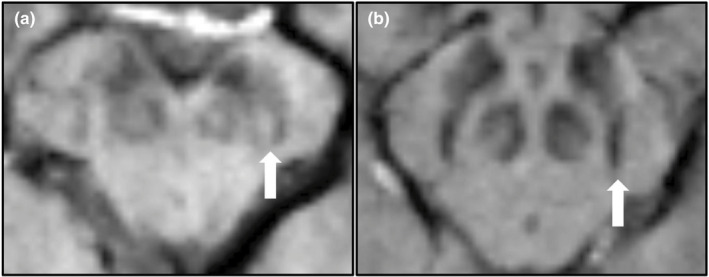
\includegraphics[width=0.8\linewidth]{FileAusiliari/Immagini/degenerative/BRB3-11-e02202-g002}
	\caption{Esempi di segno della coda di rondine (STS) in un individuo malato (a) e di STS assente in un individuo sano (b). Sono mostrate sezioni assiali del mesencefalo mappate tramite imaging pesato con suscettibilità (SWI). Le frecce bianche indicano la diversa configurazione del Nigrosoma-1 (N1). Da Brain Behav. 2021 May 24;11(7):e02202. doi: 10.1002/brb3.2202}
	\label{fig:brb3-11-e02202-g002}
\end{figure*}


La diagnosi differenziale delle sindromi parkinsoniane atipiche beneficia significativamente dell'imaging RM. L'atrofia multisistemica (MSA) evidenzia caratteristica atrofia putaminale, pontica e cerebellare, con ipointensità putaminale T2/SWI e "hot cross bun sign" pontino. La paralisi sopranucleare progressiva (PSP) manifesta atrofia mesencefalica con alterazione del rapporto mesencefalo-ponte, mentre la degenerazione corticobasale (CBD) presenta atrofia frontoparietale asimmetrica con iperintensità della sostanza bianca subcorticale.
Metodiche avanzate quali Diffusion Tensor Imaging (DTI) e risonanza magnetica funzionale (fMRI) consentono la caratterizzazione delle alterazioni microstrutturali della sostanza bianca e delle modificazioni funzionali cerebrali, sebbene la sensibilità nell'identificazione della progressione patologica e nella valutazione della risposta terapeutica necessiti ulteriore validazione. Le limitazioni metodologiche includono variabilità interindividuale e sovrapposizione dei reperti radiologici nelle diverse sindromi parkinsoniane.

\subsection{Trattamento e prognosi}

\subsection{Checklist di refertazione}

\begin{itemize}[label=$\square$] % Riquadro vuoto come simbolo
	\item Escludi altre cause di parkinsonismo (es ictus)
	\item Controlla il segnale dei nigrosomi
	\item Controlla il trofismo delle strutture sottotentoriali
\end{itemize}

\subsection{Bibliografia}
\small{
	
	
}

\note{Nota a margine}
\expl{Nota a margine colorata}
\input{Capitoli/degenerative/approccio.tex}
\input{Capitoli/degenerative/degenerative.tex}
\section{Morbo di Parkinson}

\subsection{Definizione}

\subsection{Eziologia}

\begin{figure*}[h]
	\centering
	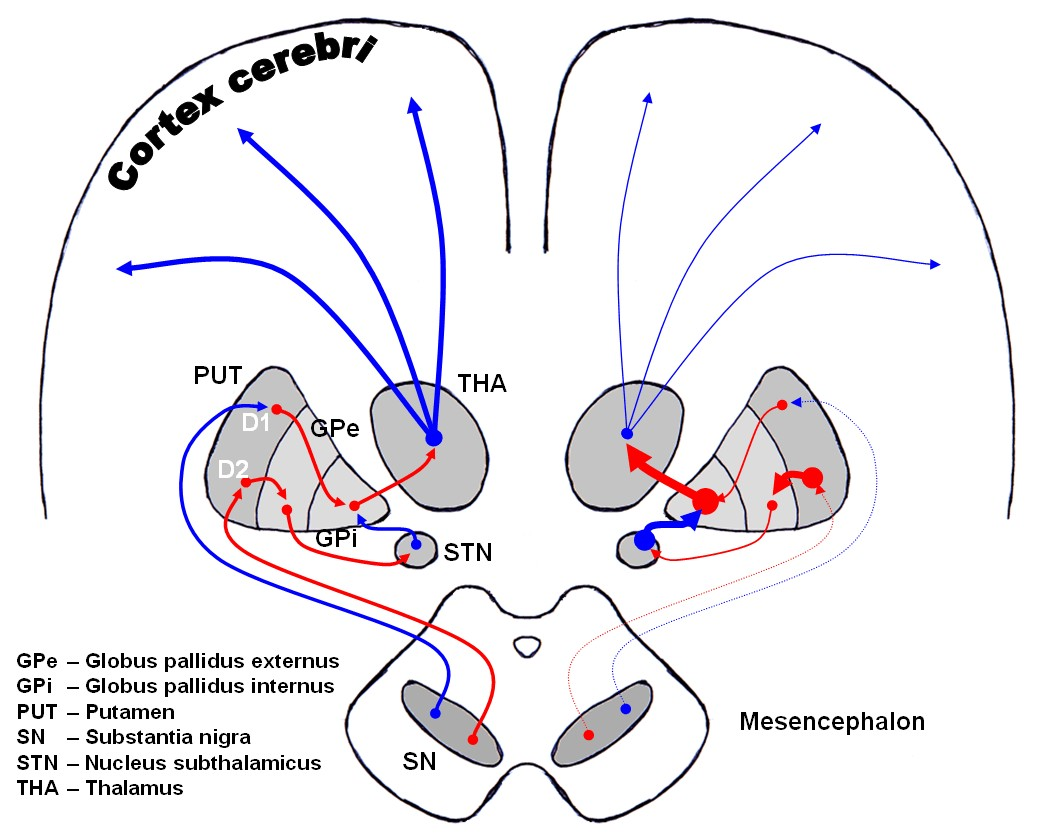
\includegraphics[width=0.5\linewidth]{FileAusiliari/Immagini/degenerative/dopamine-in-parkinsons-disease-illustration}
	\caption[Vie dopaminergiche]{L'immagine mostra le vie dopaminergiche del cervello umano in condizioni normali (a sinistra) e nella malattia di Parkinson (a destra). Le frecce rosse indicano la soppressione del bersaglio, quelle blu la stimolazione della struttura bersaglio. Caso per gentile concessione di Wikipedia, Radiopaedia.org, rID: 36286}
	\label{fig:dopamine-in-parkinsons-disease-illustration}
\end{figure*}

\subsection{Epidemiologia}
Il MP costituisce una delle principali cause di disabilità e mortalità nell'ambito delle patologie neurologiche, con una prevalenza particolarmente elevata negli Stati Uniti e in Canada (160-180 casi/100.000 abitanti). L'incidenza annuale in Nord America oscilla tra 108 e 212 casi ogni 100.000 individui di età $\geq$65 anni, con una prevalenza dello 0,3\% nella popolazione adulta $\geq$40 anni e dell'1,6\% nei soggetti ultrasessantacinquenni.
L'esordio della patologia mostra una significativa correlazione con l'età, manifestandosi tipicamente dalla quinta decade di vita, con un'età media alla diagnosi di 70,5 anni e una finestra di esordio prevalente tra i 45 e i 70 anni. Una variante giovanile può presentarsi tra i 20 e i 40 anni, sebbene l'esordio prima dei 30 anni risulti infrequente. La distribuzione per sesso evidenzia una predominanza maschile, particolarmente accentuata nella fascia d'età 50-60 anni.
L'eziologia del MP comprende fattori di rischio genetici, con particolare rilevanza nelle forme ad esordio precoce, e ambientali, tra cui l'esposizione a pesticidi e inquinanti atmosferici. Sono stati identificati fattori protettivi, inclusi il consumo di caffè, l'attività fisica e il fumo di sigaretta. La patologia si presenta prevalentemente in forma sporadica (85-90\% dei casi), mentre una minoranza dei casi (10-15\%) presenta familiarità positiva.

\subsubsection{Fattori di rischio}
L'eziopatogenesi del Morbo di Parkinson (MP) presenta una complessa interazione di fattori di rischio genetici, ambientali e non modificabili. L'anamnesi familiare positiva per MP in consanguinei di primo grado comporta un incremento del rischio relativo di 2-3 volte. Le forme monogeniche, rappresentanti meno del 10\% della casistica totale, manifestano pattern di ereditarietà autosomica dominante, recessiva o X-linked, caratterizzandosi per un esordio precoce rispetto alle forme sporadiche.
Le mutazioni eterozigoti del gene GBA1 costituiscono un significativo fattore di rischio genetico, unitamente ad alterazioni di altri geni codificanti per enzimi lisosomiali. Il coinvolgimento di geni quali SNCA, LRRK2, VPS35, Parkin, PINK1 e DJ-1 è stato ampiamente documentato. Particolare rilevanza assumono le mutazioni del gene Nurr1, determinante per l'identità neuronale dopaminergica, e del gene DJ-1, cruciale nella risposta allo stress ossidativo. Le alterazioni del gene PINK1, codificante per una chinasi mitocondriale, e del gene Park2, responsabile della sintesi della proteina parkina, sono associate a forme ad esordio precoce.
L'esposizione a neurotossine ambientali, inclusi mercurio, manganese, disolfuro di carbonio, solventi organici, MPTP e monossido di carbonio, può indurre degenerazione nigrostriatale e parkinsonismo. L'uso di neurolettici e l'abuso endovenoso di efedrone possono causare sindromi parkinsoniane potenzialmente irreversibili. Traumi cranici ripetuti, pesticidi, solventi e inquinamento atmosferico rappresentano ulteriori fattori di rischio ambientale documentati.
Tra i fattori non modificabili, l'età avanzata e il sesso maschile emergono come significativi predittori di rischio, con predominanza nella sesta decade di vita. Comorbidità quali depressione, ansia, stipsi, diabete mellito tipo 2, obesità e alterazioni del metabolismo del ferro sono state correlate a un incrementato rischio di MP.
Il consumo di tabacco e caffè, unitamente all'attività fisica regolare, ha mostrato effetti protettivi, sebbene di modesta entità. È fondamentale sottolineare che la maggioranza dei casi di MP rimane idiopatica, suggerendo un'eziologia multifattoriale.

\subsection{Presentazione  clinica}
La sintomatologia del Morbo di Parkinson manifesta un quadro clinico caratterizzato da manifestazioni motorie cardinali e sintomatologia non motoria associata. Il complesso sintomatologico motorio comprende tremore a riposo spesso asimmetrico con frequenza di 4-6 Hz, tipicamente descritto come "pill-rolling", bradicinesia manifestantesi con rallentamento motorio, ipomimia e ridotta oscillazione pendolare degli arti superiori durante la deambulazione, rigidità muscolare ("lead-pipe" o fenomeno della ruota dentata), e instabilità posturale documentabile attraverso il test della retropulsione. La deambulazione risulta caratterizzata da una progressione a piccoli passi con tendenza allo strascicamento e ridotta oscillazione degli arti superiori.
La sintomatologia accessoria include disartria con eloquio esplosivo secondario a incoordinazione linguo-diaframmatica, movimenti involontari della lingua con conseguente difficoltà protrusiva, e incremento della frequenza di ammiccamento palpebrale, quest'ultimo in contrasto con quanto osservato nella corea di Huntington. La disfunzione autonomica, i disturbi olfattivi, la sintomatologia algica, le alterazioni sensitive e i disturbi timici costituiscono il corredo sintomatologico non motorio. Il deterioramento cognitivo, con particolare coinvolgimento delle funzioni attentive, può manifestarsi e progredire nel decorso della patologia.
La progressione temporale della malattia evidenzia un esordio tipicamente unilaterale con successiva bilateralizzazione, manifestandosi prevalentemente nella sesta decade di vita. La responsività alla terapia dopaminergica, in particolare alla levodopa, rappresenta un elemento caratteristico, sebbene il tremore possa risultare farmacoresistente, in contrasto con la significativa risposta della bradicinesia e della rigidità. La variabilità fenotipica interindividuale costituisce un elemento distintivo della patologia.

\subsection{Approccio diagnostico}
L'iter diagnostico della malattia di Parkinson si fonda primariamente sulla valutazione clinica, data l'assenza di biomarcatori patognomonici. La diagnosi richiede la documentazione di bradicinesia associata ad almeno un sintomo cardine tra tremore a riposo o rigidità, valutati mediante la scala MDS-UPDRS standardizzata.
L'approccio diagnostico contempla un'accurata anamnesi ed esame obiettivo neurologico, focalizzati sull'identificazione dei sintomi cardinali: bradicinesia, tremore a riposo (4-6 Hz) tipicamente asimmetrico, rigidità e instabilità posturale. La responsività alla terapia dopaminergica, particolarmente evidente per bradicinesia e rigidità, costituisce un elemento diagnostico supportivo significativo, mentre una mancata risposta a dosaggi adeguati di levodopa suggerisce diagnosi alternative.
L'esclusione di parkinsonismi secondari richiede particolare attenzione all'insorgenza temporale dei sintomi e alla distribuzione topografica del coinvolgimento motorio. La diagnostica per immagini, sebbene non necessaria nelle presentazioni cliniche tipiche con adeguata risposta alla levodopa, può includere RM cerebrale, particolarmente utile mediante sequenze SWI per la valutazione del "swallow tail sign" nigrostriatale. La SPECT con 123I-FP-CIT (DaTscan) documenta la disfunzione dopaminergica presinaptica, mentre la PET con FDG consente la differenziazione metabolica tra PD e sindromi parkinsoniane atipiche.
L'analisi genetica, indicata in casi selezionati (esordio precoce, familiarità positiva, specifiche etnie), e la valutazione autonomica mediante scintigrafia miocardica con MIBG, che evidenzia la denervazione simpatica caratteristica, completano l'iter diagnostico. L'ecografia transcranica può evidenziare l'iperecogenicità della sostanza nera, supportando la diagnosi differenziale.
I criteri MDS stratificano la diagnosi in PD clinicamente stabilita e probabile, bilanciando specificità e sensibilità diagnostica nella pratica clinica.

\begin{Oss}
	La scala MDS-UPDRS (Movement Disorder Society-Unified Parkinson's Disease Rating Scale) è uno strumento di valutazione clinica ampiamente utilizzato per quantificare la gravità dei sintomi motori e non motori della malattia di Parkinson. Questa scala è stata sviluppata per migliorare la consistenza nella valutazione dei sintomi e per integrare meglio gli aspetti non motori della PD.
	Struttura: La scala MDS-UPDRS è composta da quattro sezioni:
	\begin{description}
		\item[Sezione I]{Esperienze non motorie della vita quotidiana. Questa sezione valuta aspetti come le capacità cognitive, i disturbi comportamentali e dell'umore}
		\item [Sezione II]{Esperienze motorie della vita quotidiana. Questa sezione valuta l'impatto dei sintomi motori sulle attività quotidiane}
		\item [Sezione III]{Esame motorio. Questa sezione valuta i segni motori della PD attraverso un esame clinico, come il tremore, la rigidità e la bradicinesia}
		\item[Sezione IV]{Complicanze della terapia. Questa sezione valuta le complicanze associate al trattamento farmacologico}
	\end{description}
	Il punteggio totale per le sezioni I-IV varia da 0 (nessuna disabilità) a 199 (disabilità totale). La sezione III, che valuta i sintomi motori, ha un punteggio che varia da 0 a 132.
	Oltre alla scala MDS-UPDRS, esistono altre scale di valutazione utilizzate nella PD, come la scala di Hoehn e Yahr e la scala di Schwab e England. La scala di Hoehn e Yahr valuta la gravità della malattia da 0 (nessuna malattia) a 5 (paziente costretto su sedia a rotelle o allettato senza assistenza).
\end{Oss}

\subsection{Anatomia patologica}
Dal punto di vista anatomopatologico il morbo di Parkinson si manifesta attraverso inclusioni proteiche intraneuronali denominate corpi di Lewy, costituiti primariamente da aggregati patologici di alfa-sinucleina, una proteina sinaptica fisiologicamente presente nel sistema nervoso centrale. L'accumulo di queste inclusioni, sebbene non patognomonico del morbo di Parkinson essendo documentabile anche nella demenza a corpi di Lewy, rappresenta una caratteristica istopatologica fondamentale quando localizzato nella substantia nigra, in associazione alla perdita neuronale dopaminergica. L'assenza di corpi di Lewy nelle forme post-encefalitiche, caratterizzate invece da grovigli neurofibrillari, e in alcune forme geneticamente determinate, sottolinea l'eterogeneità patogenetica della malattia.
La progressione spazio-temporale della patologia, codificata nello staging di Braak, delinea sei stadi evolutivi caratterizzati da una diffusione ascendente delle alterazioni neuropatologiche. Gli stadi iniziali (1-2) coinvolgono il nucleo motore dorsale dei nervi glossofaringeo e vago e il nucleo olfattivo anteriore, precedendo frequentemente la sintomatologia motoria. Gli stadi intermedi (3-4) documentano il coinvolgimento della substantia nigra pars compacta, del prosencefalo basale e della mesocorteccia temporale, correlando con l'esordio clinico della malattia. Gli stadi terminali (5-6) evidenziano una progressione neocorticale diffusa.
La patogenesi molecolare implica alterazioni del metabolismo dell'alfa-sinucleina, potenzialmente accelerate da disfunzioni delle proteine heat shock o dall'azione della dopamina. Il coinvolgimento della proteina parkin nella degradazione proteasomica evidenzia meccanismi neurodegenerativi potenzialmente indipendenti dalla formazione dei corpi di Lewy.
L'alfa-sinucleina, proteina fisiologicamente localizzata nelle terminazioni presinaptiche neuronali, manifesta nella patogenesi del morbo di Parkinson un processo patologico caratterizzato da misfolding proteico e successiva aggregazione in oligomeri, protofibrille e fibrille, culminante nella formazione dei corpi di Lewy intraneuronali. Questi aggregati proteici, considerati hallmark istopatologico della malattia, evidenziano particolare neurotossicità nella forma protofibrillare, determinando disfunzione e successiva degenerazione neuronale dopaminergica nigrostriatale.
L'identificazione di mutazioni nel gene SNCA, codificante per l'alfa-sinucleina, nelle forme familiari di malattia, unitamente alla documentazione di fenotipi clinici particolarmente aggressivi in presenza di duplicazione o triplicazione genica, ha fornito evidenze significative del ruolo causale di questa proteina nella patogenesi della malattia. La documentata capacità di trasmissione transcellulare dell'alfa-sinucleina patologica costituisce il substrato molecolare della progressione anatomopatologica descritta nello staging di Braak.
La disfunzione sinaptica correlata all'accumulo di alfa-sinucleina rappresenta un meccanismo patogenetico critico, modulato da fattori quali stress ossidativo, alterazioni del sistema ubiquitina-proteasoma e interazione con il metabolismo dopaminergico. Mutazioni nei geni parkin, PINK1 e DJ-1 influenzano il metabolismo dell'alfa-sinucleina attraverso alterazioni dei sistemi di degradazione proteica.
L'alfa-sinucleina costituisce attualmente un promettente target terapeutico, con particolare interesse per lo sviluppo di anticorpi monoclonali specifici e inibitori dell'aggregazione proteica, finalizzati al rallentamento della progressione patologica.

\subsection{Imaging}

\subsubsection{TC}
La TC manifesta un'utilità clinica circoscritta nella valutazione diagnostica primaria del MP, assumendo rilevanza nell'esclusione di patologie strutturali mimiche quali lesioni espansive, idrocefalo o alterazioni vascolari, particolarmente in presenza di presentazioni cliniche atipiche o "red flags" suggestive di diagnosi alternative.
Nel contesto della gestione terapeutica, la TC assume particolare rilevanza nella valutazione post-chirurgica della stimolazione cerebrale profonda (DBS), consentendo la verifica del corretto posizionamento degli elettrodi nel nucleo subtalamico (STN), tipicamente localizzati a 9mm dalla linea mediana, e l'identificazione di eventuali complicanze post-procedurali quali eventi emorragici, ischemici o fenomeni infiammatori transitori, questi ultimi caratterizzati da aree ipodense perilettrodiche a risoluzione graduale. L'utilità della metodica nel follow-up routinario post-DBS risulta secondaria.
La sensibilità subottimale della TC nella diagnosi differenziale tra PD e sindromi parkinsoniane atipiche, incluse atrofia multisistemica e paralisi sopranucleare progressiva, nonché nella distinzione dal tremore essenziale, ne limita significativamente l'applicazione clinica in questo contesto diagnostico.

\subsubsection{RM}
La RM è frequentemente normale nelle sequenze convenzionali (T1, T2, FLAIR) nelle fasi iniziali di malattia. L'implementazione di sequenze susceptibility-weighted imaging (SWI) o T2*-weighted ad alta risoluzione consente la visualizzazione del nigrosoma-1, struttura caratterizzata dal patognomonico "swallow tail sign", la cui perdita correla con la degenerazione dopaminergica nigrostriatale. L'accumulo patologico di ferro nella substantia nigra, quantificabile mediante sequenze SWI/T2* e incrementato del 50\% rispetto ai controlli, costituisce un ulteriore marker diagnostico, complementato dall'imaging della neuromelanina mediante sequenze T1 con impulsi di trasferimento di magnetizzazione (MTC).

\begin{figure*}[h]
	\centering
	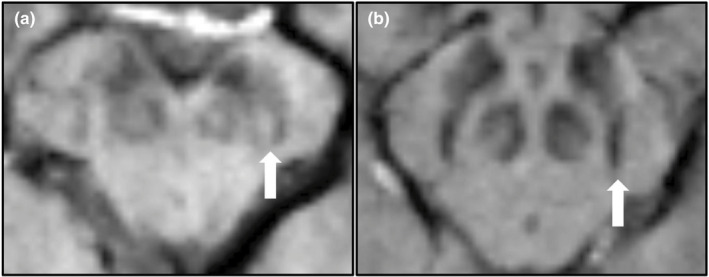
\includegraphics[width=0.8\linewidth]{FileAusiliari/Immagini/degenerative/BRB3-11-e02202-g002}
	\caption{Esempi di segno della coda di rondine (STS) in un individuo malato (a) e di STS assente in un individuo sano (b). Sono mostrate sezioni assiali del mesencefalo mappate tramite imaging pesato con suscettibilità (SWI). Le frecce bianche indicano la diversa configurazione del Nigrosoma-1 (N1). Da Brain Behav. 2021 May 24;11(7):e02202. doi: 10.1002/brb3.2202}
	\label{fig:brb3-11-e02202-g002}
\end{figure*}


La diagnosi differenziale delle sindromi parkinsoniane atipiche beneficia significativamente dell'imaging RM. L'atrofia multisistemica (MSA) evidenzia caratteristica atrofia putaminale, pontica e cerebellare, con ipointensità putaminale T2/SWI e "hot cross bun sign" pontino. La paralisi sopranucleare progressiva (PSP) manifesta atrofia mesencefalica con alterazione del rapporto mesencefalo-ponte, mentre la degenerazione corticobasale (CBD) presenta atrofia frontoparietale asimmetrica con iperintensità della sostanza bianca subcorticale.
Metodiche avanzate quali Diffusion Tensor Imaging (DTI) e risonanza magnetica funzionale (fMRI) consentono la caratterizzazione delle alterazioni microstrutturali della sostanza bianca e delle modificazioni funzionali cerebrali, sebbene la sensibilità nell'identificazione della progressione patologica e nella valutazione della risposta terapeutica necessiti ulteriore validazione. Le limitazioni metodologiche includono variabilità interindividuale e sovrapposizione dei reperti radiologici nelle diverse sindromi parkinsoniane.

\subsection{Trattamento e prognosi}

\subsection{Checklist di refertazione}

\begin{itemize}[label=$\square$] % Riquadro vuoto come simbolo
	\item Escludi altre cause di parkinsonismo (es ictus)
	\item Controlla il segnale dei nigrosomi
	\item Controlla il trofismo delle strutture sottotentoriali
\end{itemize}

\subsection{Bibliografia}
\small{
	
	
}

\note{Nota a margine}
\expl{Nota a margine colorata}
\input{Capitoli/degenerative/approccio.tex}
\input{Capitoli/degenerative/degenerative.tex}
\section{Morbo di Parkinson}

\subsection{Definizione}

\subsection{Eziologia}

\begin{figure*}[h]
	\centering
	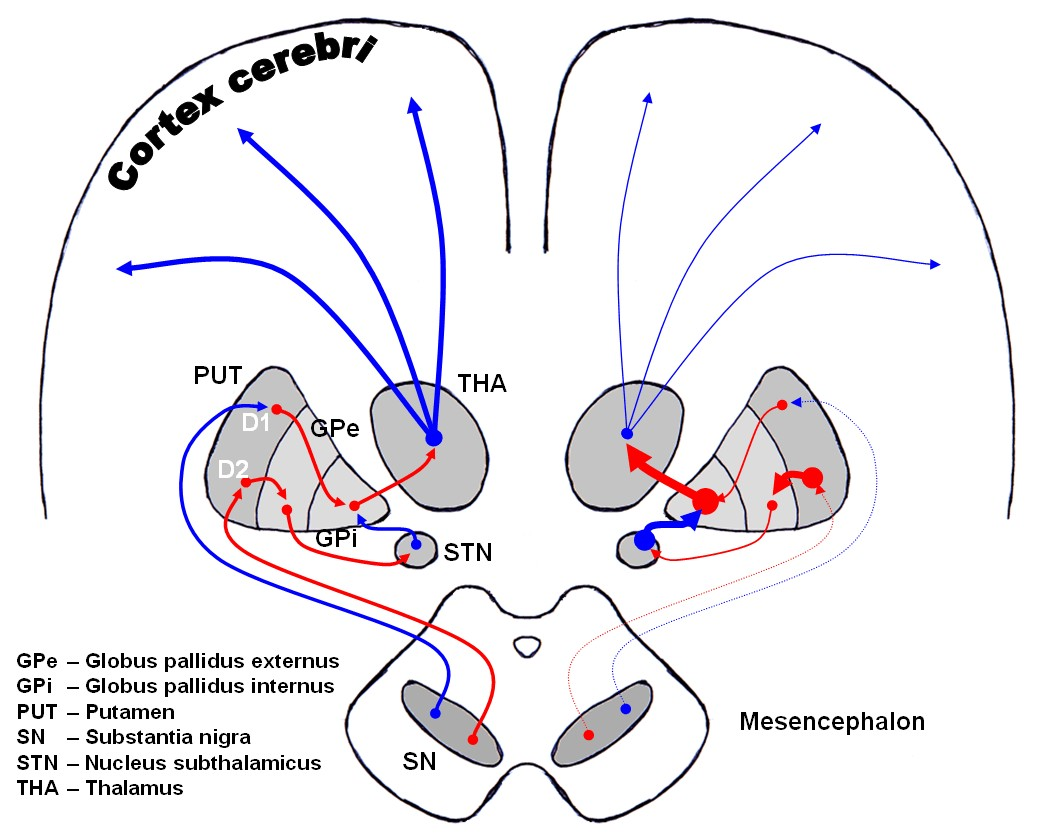
\includegraphics[width=0.5\linewidth]{FileAusiliari/Immagini/degenerative/dopamine-in-parkinsons-disease-illustration}
	\caption[Vie dopaminergiche]{L'immagine mostra le vie dopaminergiche del cervello umano in condizioni normali (a sinistra) e nella malattia di Parkinson (a destra). Le frecce rosse indicano la soppressione del bersaglio, quelle blu la stimolazione della struttura bersaglio. Caso per gentile concessione di Wikipedia, Radiopaedia.org, rID: 36286}
	\label{fig:dopamine-in-parkinsons-disease-illustration}
\end{figure*}

\subsection{Epidemiologia}
Il MP costituisce una delle principali cause di disabilità e mortalità nell'ambito delle patologie neurologiche, con una prevalenza particolarmente elevata negli Stati Uniti e in Canada (160-180 casi/100.000 abitanti). L'incidenza annuale in Nord America oscilla tra 108 e 212 casi ogni 100.000 individui di età $\geq$65 anni, con una prevalenza dello 0,3\% nella popolazione adulta $\geq$40 anni e dell'1,6\% nei soggetti ultrasessantacinquenni.
L'esordio della patologia mostra una significativa correlazione con l'età, manifestandosi tipicamente dalla quinta decade di vita, con un'età media alla diagnosi di 70,5 anni e una finestra di esordio prevalente tra i 45 e i 70 anni. Una variante giovanile può presentarsi tra i 20 e i 40 anni, sebbene l'esordio prima dei 30 anni risulti infrequente. La distribuzione per sesso evidenzia una predominanza maschile, particolarmente accentuata nella fascia d'età 50-60 anni.
L'eziologia del MP comprende fattori di rischio genetici, con particolare rilevanza nelle forme ad esordio precoce, e ambientali, tra cui l'esposizione a pesticidi e inquinanti atmosferici. Sono stati identificati fattori protettivi, inclusi il consumo di caffè, l'attività fisica e il fumo di sigaretta. La patologia si presenta prevalentemente in forma sporadica (85-90\% dei casi), mentre una minoranza dei casi (10-15\%) presenta familiarità positiva.

\subsubsection{Fattori di rischio}
L'eziopatogenesi del Morbo di Parkinson (MP) presenta una complessa interazione di fattori di rischio genetici, ambientali e non modificabili. L'anamnesi familiare positiva per MP in consanguinei di primo grado comporta un incremento del rischio relativo di 2-3 volte. Le forme monogeniche, rappresentanti meno del 10\% della casistica totale, manifestano pattern di ereditarietà autosomica dominante, recessiva o X-linked, caratterizzandosi per un esordio precoce rispetto alle forme sporadiche.
Le mutazioni eterozigoti del gene GBA1 costituiscono un significativo fattore di rischio genetico, unitamente ad alterazioni di altri geni codificanti per enzimi lisosomiali. Il coinvolgimento di geni quali SNCA, LRRK2, VPS35, Parkin, PINK1 e DJ-1 è stato ampiamente documentato. Particolare rilevanza assumono le mutazioni del gene Nurr1, determinante per l'identità neuronale dopaminergica, e del gene DJ-1, cruciale nella risposta allo stress ossidativo. Le alterazioni del gene PINK1, codificante per una chinasi mitocondriale, e del gene Park2, responsabile della sintesi della proteina parkina, sono associate a forme ad esordio precoce.
L'esposizione a neurotossine ambientali, inclusi mercurio, manganese, disolfuro di carbonio, solventi organici, MPTP e monossido di carbonio, può indurre degenerazione nigrostriatale e parkinsonismo. L'uso di neurolettici e l'abuso endovenoso di efedrone possono causare sindromi parkinsoniane potenzialmente irreversibili. Traumi cranici ripetuti, pesticidi, solventi e inquinamento atmosferico rappresentano ulteriori fattori di rischio ambientale documentati.
Tra i fattori non modificabili, l'età avanzata e il sesso maschile emergono come significativi predittori di rischio, con predominanza nella sesta decade di vita. Comorbidità quali depressione, ansia, stipsi, diabete mellito tipo 2, obesità e alterazioni del metabolismo del ferro sono state correlate a un incrementato rischio di MP.
Il consumo di tabacco e caffè, unitamente all'attività fisica regolare, ha mostrato effetti protettivi, sebbene di modesta entità. È fondamentale sottolineare che la maggioranza dei casi di MP rimane idiopatica, suggerendo un'eziologia multifattoriale.

\subsection{Presentazione  clinica}
La sintomatologia del Morbo di Parkinson manifesta un quadro clinico caratterizzato da manifestazioni motorie cardinali e sintomatologia non motoria associata. Il complesso sintomatologico motorio comprende tremore a riposo spesso asimmetrico con frequenza di 4-6 Hz, tipicamente descritto come "pill-rolling", bradicinesia manifestantesi con rallentamento motorio, ipomimia e ridotta oscillazione pendolare degli arti superiori durante la deambulazione, rigidità muscolare ("lead-pipe" o fenomeno della ruota dentata), e instabilità posturale documentabile attraverso il test della retropulsione. La deambulazione risulta caratterizzata da una progressione a piccoli passi con tendenza allo strascicamento e ridotta oscillazione degli arti superiori.
La sintomatologia accessoria include disartria con eloquio esplosivo secondario a incoordinazione linguo-diaframmatica, movimenti involontari della lingua con conseguente difficoltà protrusiva, e incremento della frequenza di ammiccamento palpebrale, quest'ultimo in contrasto con quanto osservato nella corea di Huntington. La disfunzione autonomica, i disturbi olfattivi, la sintomatologia algica, le alterazioni sensitive e i disturbi timici costituiscono il corredo sintomatologico non motorio. Il deterioramento cognitivo, con particolare coinvolgimento delle funzioni attentive, può manifestarsi e progredire nel decorso della patologia.
La progressione temporale della malattia evidenzia un esordio tipicamente unilaterale con successiva bilateralizzazione, manifestandosi prevalentemente nella sesta decade di vita. La responsività alla terapia dopaminergica, in particolare alla levodopa, rappresenta un elemento caratteristico, sebbene il tremore possa risultare farmacoresistente, in contrasto con la significativa risposta della bradicinesia e della rigidità. La variabilità fenotipica interindividuale costituisce un elemento distintivo della patologia.

\subsection{Approccio diagnostico}
L'iter diagnostico della malattia di Parkinson si fonda primariamente sulla valutazione clinica, data l'assenza di biomarcatori patognomonici. La diagnosi richiede la documentazione di bradicinesia associata ad almeno un sintomo cardine tra tremore a riposo o rigidità, valutati mediante la scala MDS-UPDRS standardizzata.
L'approccio diagnostico contempla un'accurata anamnesi ed esame obiettivo neurologico, focalizzati sull'identificazione dei sintomi cardinali: bradicinesia, tremore a riposo (4-6 Hz) tipicamente asimmetrico, rigidità e instabilità posturale. La responsività alla terapia dopaminergica, particolarmente evidente per bradicinesia e rigidità, costituisce un elemento diagnostico supportivo significativo, mentre una mancata risposta a dosaggi adeguati di levodopa suggerisce diagnosi alternative.
L'esclusione di parkinsonismi secondari richiede particolare attenzione all'insorgenza temporale dei sintomi e alla distribuzione topografica del coinvolgimento motorio. La diagnostica per immagini, sebbene non necessaria nelle presentazioni cliniche tipiche con adeguata risposta alla levodopa, può includere RM cerebrale, particolarmente utile mediante sequenze SWI per la valutazione del "swallow tail sign" nigrostriatale. La SPECT con 123I-FP-CIT (DaTscan) documenta la disfunzione dopaminergica presinaptica, mentre la PET con FDG consente la differenziazione metabolica tra PD e sindromi parkinsoniane atipiche.
L'analisi genetica, indicata in casi selezionati (esordio precoce, familiarità positiva, specifiche etnie), e la valutazione autonomica mediante scintigrafia miocardica con MIBG, che evidenzia la denervazione simpatica caratteristica, completano l'iter diagnostico. L'ecografia transcranica può evidenziare l'iperecogenicità della sostanza nera, supportando la diagnosi differenziale.
I criteri MDS stratificano la diagnosi in PD clinicamente stabilita e probabile, bilanciando specificità e sensibilità diagnostica nella pratica clinica.

\begin{Oss}
	La scala MDS-UPDRS (Movement Disorder Society-Unified Parkinson's Disease Rating Scale) è uno strumento di valutazione clinica ampiamente utilizzato per quantificare la gravità dei sintomi motori e non motori della malattia di Parkinson. Questa scala è stata sviluppata per migliorare la consistenza nella valutazione dei sintomi e per integrare meglio gli aspetti non motori della PD.
	Struttura: La scala MDS-UPDRS è composta da quattro sezioni:
	\begin{description}
		\item[Sezione I]{Esperienze non motorie della vita quotidiana. Questa sezione valuta aspetti come le capacità cognitive, i disturbi comportamentali e dell'umore}
		\item [Sezione II]{Esperienze motorie della vita quotidiana. Questa sezione valuta l'impatto dei sintomi motori sulle attività quotidiane}
		\item [Sezione III]{Esame motorio. Questa sezione valuta i segni motori della PD attraverso un esame clinico, come il tremore, la rigidità e la bradicinesia}
		\item[Sezione IV]{Complicanze della terapia. Questa sezione valuta le complicanze associate al trattamento farmacologico}
	\end{description}
	Il punteggio totale per le sezioni I-IV varia da 0 (nessuna disabilità) a 199 (disabilità totale). La sezione III, che valuta i sintomi motori, ha un punteggio che varia da 0 a 132.
	Oltre alla scala MDS-UPDRS, esistono altre scale di valutazione utilizzate nella PD, come la scala di Hoehn e Yahr e la scala di Schwab e England. La scala di Hoehn e Yahr valuta la gravità della malattia da 0 (nessuna malattia) a 5 (paziente costretto su sedia a rotelle o allettato senza assistenza).
\end{Oss}

\subsection{Anatomia patologica}
Dal punto di vista anatomopatologico il morbo di Parkinson si manifesta attraverso inclusioni proteiche intraneuronali denominate corpi di Lewy, costituiti primariamente da aggregati patologici di alfa-sinucleina, una proteina sinaptica fisiologicamente presente nel sistema nervoso centrale. L'accumulo di queste inclusioni, sebbene non patognomonico del morbo di Parkinson essendo documentabile anche nella demenza a corpi di Lewy, rappresenta una caratteristica istopatologica fondamentale quando localizzato nella substantia nigra, in associazione alla perdita neuronale dopaminergica. L'assenza di corpi di Lewy nelle forme post-encefalitiche, caratterizzate invece da grovigli neurofibrillari, e in alcune forme geneticamente determinate, sottolinea l'eterogeneità patogenetica della malattia.
La progressione spazio-temporale della patologia, codificata nello staging di Braak, delinea sei stadi evolutivi caratterizzati da una diffusione ascendente delle alterazioni neuropatologiche. Gli stadi iniziali (1-2) coinvolgono il nucleo motore dorsale dei nervi glossofaringeo e vago e il nucleo olfattivo anteriore, precedendo frequentemente la sintomatologia motoria. Gli stadi intermedi (3-4) documentano il coinvolgimento della substantia nigra pars compacta, del prosencefalo basale e della mesocorteccia temporale, correlando con l'esordio clinico della malattia. Gli stadi terminali (5-6) evidenziano una progressione neocorticale diffusa.
La patogenesi molecolare implica alterazioni del metabolismo dell'alfa-sinucleina, potenzialmente accelerate da disfunzioni delle proteine heat shock o dall'azione della dopamina. Il coinvolgimento della proteina parkin nella degradazione proteasomica evidenzia meccanismi neurodegenerativi potenzialmente indipendenti dalla formazione dei corpi di Lewy.
L'alfa-sinucleina, proteina fisiologicamente localizzata nelle terminazioni presinaptiche neuronali, manifesta nella patogenesi del morbo di Parkinson un processo patologico caratterizzato da misfolding proteico e successiva aggregazione in oligomeri, protofibrille e fibrille, culminante nella formazione dei corpi di Lewy intraneuronali. Questi aggregati proteici, considerati hallmark istopatologico della malattia, evidenziano particolare neurotossicità nella forma protofibrillare, determinando disfunzione e successiva degenerazione neuronale dopaminergica nigrostriatale.
L'identificazione di mutazioni nel gene SNCA, codificante per l'alfa-sinucleina, nelle forme familiari di malattia, unitamente alla documentazione di fenotipi clinici particolarmente aggressivi in presenza di duplicazione o triplicazione genica, ha fornito evidenze significative del ruolo causale di questa proteina nella patogenesi della malattia. La documentata capacità di trasmissione transcellulare dell'alfa-sinucleina patologica costituisce il substrato molecolare della progressione anatomopatologica descritta nello staging di Braak.
La disfunzione sinaptica correlata all'accumulo di alfa-sinucleina rappresenta un meccanismo patogenetico critico, modulato da fattori quali stress ossidativo, alterazioni del sistema ubiquitina-proteasoma e interazione con il metabolismo dopaminergico. Mutazioni nei geni parkin, PINK1 e DJ-1 influenzano il metabolismo dell'alfa-sinucleina attraverso alterazioni dei sistemi di degradazione proteica.
L'alfa-sinucleina costituisce attualmente un promettente target terapeutico, con particolare interesse per lo sviluppo di anticorpi monoclonali specifici e inibitori dell'aggregazione proteica, finalizzati al rallentamento della progressione patologica.

\subsection{Imaging}

\subsubsection{TC}
La TC manifesta un'utilità clinica circoscritta nella valutazione diagnostica primaria del MP, assumendo rilevanza nell'esclusione di patologie strutturali mimiche quali lesioni espansive, idrocefalo o alterazioni vascolari, particolarmente in presenza di presentazioni cliniche atipiche o "red flags" suggestive di diagnosi alternative.
Nel contesto della gestione terapeutica, la TC assume particolare rilevanza nella valutazione post-chirurgica della stimolazione cerebrale profonda (DBS), consentendo la verifica del corretto posizionamento degli elettrodi nel nucleo subtalamico (STN), tipicamente localizzati a 9mm dalla linea mediana, e l'identificazione di eventuali complicanze post-procedurali quali eventi emorragici, ischemici o fenomeni infiammatori transitori, questi ultimi caratterizzati da aree ipodense perilettrodiche a risoluzione graduale. L'utilità della metodica nel follow-up routinario post-DBS risulta secondaria.
La sensibilità subottimale della TC nella diagnosi differenziale tra PD e sindromi parkinsoniane atipiche, incluse atrofia multisistemica e paralisi sopranucleare progressiva, nonché nella distinzione dal tremore essenziale, ne limita significativamente l'applicazione clinica in questo contesto diagnostico.

\subsubsection{RM}
La RM è frequentemente normale nelle sequenze convenzionali (T1, T2, FLAIR) nelle fasi iniziali di malattia. L'implementazione di sequenze susceptibility-weighted imaging (SWI) o T2*-weighted ad alta risoluzione consente la visualizzazione del nigrosoma-1, struttura caratterizzata dal patognomonico "swallow tail sign", la cui perdita correla con la degenerazione dopaminergica nigrostriatale. L'accumulo patologico di ferro nella substantia nigra, quantificabile mediante sequenze SWI/T2* e incrementato del 50\% rispetto ai controlli, costituisce un ulteriore marker diagnostico, complementato dall'imaging della neuromelanina mediante sequenze T1 con impulsi di trasferimento di magnetizzazione (MTC).

\begin{figure*}[h]
	\centering
	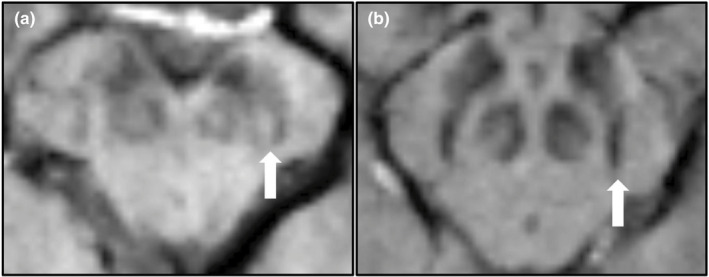
\includegraphics[width=0.8\linewidth]{FileAusiliari/Immagini/degenerative/BRB3-11-e02202-g002}
	\caption{Esempi di segno della coda di rondine (STS) in un individuo malato (a) e di STS assente in un individuo sano (b). Sono mostrate sezioni assiali del mesencefalo mappate tramite imaging pesato con suscettibilità (SWI). Le frecce bianche indicano la diversa configurazione del Nigrosoma-1 (N1). Da Brain Behav. 2021 May 24;11(7):e02202. doi: 10.1002/brb3.2202}
	\label{fig:brb3-11-e02202-g002}
\end{figure*}


La diagnosi differenziale delle sindromi parkinsoniane atipiche beneficia significativamente dell'imaging RM. L'atrofia multisistemica (MSA) evidenzia caratteristica atrofia putaminale, pontica e cerebellare, con ipointensità putaminale T2/SWI e "hot cross bun sign" pontino. La paralisi sopranucleare progressiva (PSP) manifesta atrofia mesencefalica con alterazione del rapporto mesencefalo-ponte, mentre la degenerazione corticobasale (CBD) presenta atrofia frontoparietale asimmetrica con iperintensità della sostanza bianca subcorticale.
Metodiche avanzate quali Diffusion Tensor Imaging (DTI) e risonanza magnetica funzionale (fMRI) consentono la caratterizzazione delle alterazioni microstrutturali della sostanza bianca e delle modificazioni funzionali cerebrali, sebbene la sensibilità nell'identificazione della progressione patologica e nella valutazione della risposta terapeutica necessiti ulteriore validazione. Le limitazioni metodologiche includono variabilità interindividuale e sovrapposizione dei reperti radiologici nelle diverse sindromi parkinsoniane.

\subsection{Trattamento e prognosi}

\subsection{Checklist di refertazione}

\begin{itemize}[label=$\square$] % Riquadro vuoto come simbolo
	\item Escludi altre cause di parkinsonismo (es ictus)
	\item Controlla il segnale dei nigrosomi
	\item Controlla il trofismo delle strutture sottotentoriali
\end{itemize}

\subsection{Bibliografia}
\small{
	
	
}

\note{Nota a margine}
\expl{Nota a margine colorata}
\input{Capitoli/degenerative/approccio.tex}
\input{Capitoli/degenerative/degenerative.tex}
\section{Morbo di Parkinson}

\subsection{Definizione}

\subsection{Eziologia}

\begin{figure*}[h]
	\centering
	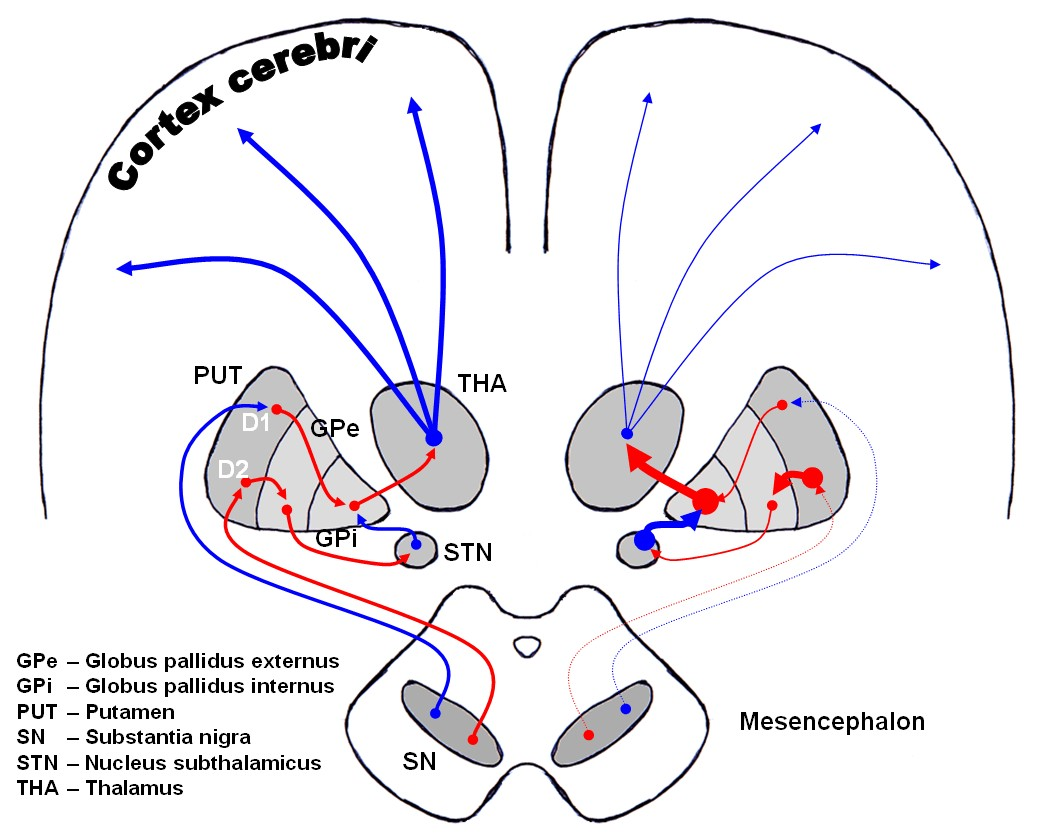
\includegraphics[width=0.5\linewidth]{FileAusiliari/Immagini/degenerative/dopamine-in-parkinsons-disease-illustration}
	\caption[Vie dopaminergiche]{L'immagine mostra le vie dopaminergiche del cervello umano in condizioni normali (a sinistra) e nella malattia di Parkinson (a destra). Le frecce rosse indicano la soppressione del bersaglio, quelle blu la stimolazione della struttura bersaglio. Caso per gentile concessione di Wikipedia, Radiopaedia.org, rID: 36286}
	\label{fig:dopamine-in-parkinsons-disease-illustration}
\end{figure*}

\subsection{Epidemiologia}
Il MP costituisce una delle principali cause di disabilità e mortalità nell'ambito delle patologie neurologiche, con una prevalenza particolarmente elevata negli Stati Uniti e in Canada (160-180 casi/100.000 abitanti). L'incidenza annuale in Nord America oscilla tra 108 e 212 casi ogni 100.000 individui di età $\geq$65 anni, con una prevalenza dello 0,3\% nella popolazione adulta $\geq$40 anni e dell'1,6\% nei soggetti ultrasessantacinquenni.
L'esordio della patologia mostra una significativa correlazione con l'età, manifestandosi tipicamente dalla quinta decade di vita, con un'età media alla diagnosi di 70,5 anni e una finestra di esordio prevalente tra i 45 e i 70 anni. Una variante giovanile può presentarsi tra i 20 e i 40 anni, sebbene l'esordio prima dei 30 anni risulti infrequente. La distribuzione per sesso evidenzia una predominanza maschile, particolarmente accentuata nella fascia d'età 50-60 anni.
L'eziologia del MP comprende fattori di rischio genetici, con particolare rilevanza nelle forme ad esordio precoce, e ambientali, tra cui l'esposizione a pesticidi e inquinanti atmosferici. Sono stati identificati fattori protettivi, inclusi il consumo di caffè, l'attività fisica e il fumo di sigaretta. La patologia si presenta prevalentemente in forma sporadica (85-90\% dei casi), mentre una minoranza dei casi (10-15\%) presenta familiarità positiva.

\subsubsection{Fattori di rischio}
L'eziopatogenesi del Morbo di Parkinson (MP) presenta una complessa interazione di fattori di rischio genetici, ambientali e non modificabili. L'anamnesi familiare positiva per MP in consanguinei di primo grado comporta un incremento del rischio relativo di 2-3 volte. Le forme monogeniche, rappresentanti meno del 10\% della casistica totale, manifestano pattern di ereditarietà autosomica dominante, recessiva o X-linked, caratterizzandosi per un esordio precoce rispetto alle forme sporadiche.
Le mutazioni eterozigoti del gene GBA1 costituiscono un significativo fattore di rischio genetico, unitamente ad alterazioni di altri geni codificanti per enzimi lisosomiali. Il coinvolgimento di geni quali SNCA, LRRK2, VPS35, Parkin, PINK1 e DJ-1 è stato ampiamente documentato. Particolare rilevanza assumono le mutazioni del gene Nurr1, determinante per l'identità neuronale dopaminergica, e del gene DJ-1, cruciale nella risposta allo stress ossidativo. Le alterazioni del gene PINK1, codificante per una chinasi mitocondriale, e del gene Park2, responsabile della sintesi della proteina parkina, sono associate a forme ad esordio precoce.
L'esposizione a neurotossine ambientali, inclusi mercurio, manganese, disolfuro di carbonio, solventi organici, MPTP e monossido di carbonio, può indurre degenerazione nigrostriatale e parkinsonismo. L'uso di neurolettici e l'abuso endovenoso di efedrone possono causare sindromi parkinsoniane potenzialmente irreversibili. Traumi cranici ripetuti, pesticidi, solventi e inquinamento atmosferico rappresentano ulteriori fattori di rischio ambientale documentati.
Tra i fattori non modificabili, l'età avanzata e il sesso maschile emergono come significativi predittori di rischio, con predominanza nella sesta decade di vita. Comorbidità quali depressione, ansia, stipsi, diabete mellito tipo 2, obesità e alterazioni del metabolismo del ferro sono state correlate a un incrementato rischio di MP.
Il consumo di tabacco e caffè, unitamente all'attività fisica regolare, ha mostrato effetti protettivi, sebbene di modesta entità. È fondamentale sottolineare che la maggioranza dei casi di MP rimane idiopatica, suggerendo un'eziologia multifattoriale.

\subsection{Presentazione  clinica}
La sintomatologia del Morbo di Parkinson manifesta un quadro clinico caratterizzato da manifestazioni motorie cardinali e sintomatologia non motoria associata. Il complesso sintomatologico motorio comprende tremore a riposo spesso asimmetrico con frequenza di 4-6 Hz, tipicamente descritto come "pill-rolling", bradicinesia manifestantesi con rallentamento motorio, ipomimia e ridotta oscillazione pendolare degli arti superiori durante la deambulazione, rigidità muscolare ("lead-pipe" o fenomeno della ruota dentata), e instabilità posturale documentabile attraverso il test della retropulsione. La deambulazione risulta caratterizzata da una progressione a piccoli passi con tendenza allo strascicamento e ridotta oscillazione degli arti superiori.
La sintomatologia accessoria include disartria con eloquio esplosivo secondario a incoordinazione linguo-diaframmatica, movimenti involontari della lingua con conseguente difficoltà protrusiva, e incremento della frequenza di ammiccamento palpebrale, quest'ultimo in contrasto con quanto osservato nella corea di Huntington. La disfunzione autonomica, i disturbi olfattivi, la sintomatologia algica, le alterazioni sensitive e i disturbi timici costituiscono il corredo sintomatologico non motorio. Il deterioramento cognitivo, con particolare coinvolgimento delle funzioni attentive, può manifestarsi e progredire nel decorso della patologia.
La progressione temporale della malattia evidenzia un esordio tipicamente unilaterale con successiva bilateralizzazione, manifestandosi prevalentemente nella sesta decade di vita. La responsività alla terapia dopaminergica, in particolare alla levodopa, rappresenta un elemento caratteristico, sebbene il tremore possa risultare farmacoresistente, in contrasto con la significativa risposta della bradicinesia e della rigidità. La variabilità fenotipica interindividuale costituisce un elemento distintivo della patologia.

\subsection{Approccio diagnostico}
L'iter diagnostico della malattia di Parkinson si fonda primariamente sulla valutazione clinica, data l'assenza di biomarcatori patognomonici. La diagnosi richiede la documentazione di bradicinesia associata ad almeno un sintomo cardine tra tremore a riposo o rigidità, valutati mediante la scala MDS-UPDRS standardizzata.
L'approccio diagnostico contempla un'accurata anamnesi ed esame obiettivo neurologico, focalizzati sull'identificazione dei sintomi cardinali: bradicinesia, tremore a riposo (4-6 Hz) tipicamente asimmetrico, rigidità e instabilità posturale. La responsività alla terapia dopaminergica, particolarmente evidente per bradicinesia e rigidità, costituisce un elemento diagnostico supportivo significativo, mentre una mancata risposta a dosaggi adeguati di levodopa suggerisce diagnosi alternative.
L'esclusione di parkinsonismi secondari richiede particolare attenzione all'insorgenza temporale dei sintomi e alla distribuzione topografica del coinvolgimento motorio. La diagnostica per immagini, sebbene non necessaria nelle presentazioni cliniche tipiche con adeguata risposta alla levodopa, può includere RM cerebrale, particolarmente utile mediante sequenze SWI per la valutazione del "swallow tail sign" nigrostriatale. La SPECT con 123I-FP-CIT (DaTscan) documenta la disfunzione dopaminergica presinaptica, mentre la PET con FDG consente la differenziazione metabolica tra PD e sindromi parkinsoniane atipiche.
L'analisi genetica, indicata in casi selezionati (esordio precoce, familiarità positiva, specifiche etnie), e la valutazione autonomica mediante scintigrafia miocardica con MIBG, che evidenzia la denervazione simpatica caratteristica, completano l'iter diagnostico. L'ecografia transcranica può evidenziare l'iperecogenicità della sostanza nera, supportando la diagnosi differenziale.
I criteri MDS stratificano la diagnosi in PD clinicamente stabilita e probabile, bilanciando specificità e sensibilità diagnostica nella pratica clinica.

\begin{Oss}
	La scala MDS-UPDRS (Movement Disorder Society-Unified Parkinson's Disease Rating Scale) è uno strumento di valutazione clinica ampiamente utilizzato per quantificare la gravità dei sintomi motori e non motori della malattia di Parkinson. Questa scala è stata sviluppata per migliorare la consistenza nella valutazione dei sintomi e per integrare meglio gli aspetti non motori della PD.
	Struttura: La scala MDS-UPDRS è composta da quattro sezioni:
	\begin{description}
		\item[Sezione I]{Esperienze non motorie della vita quotidiana. Questa sezione valuta aspetti come le capacità cognitive, i disturbi comportamentali e dell'umore}
		\item [Sezione II]{Esperienze motorie della vita quotidiana. Questa sezione valuta l'impatto dei sintomi motori sulle attività quotidiane}
		\item [Sezione III]{Esame motorio. Questa sezione valuta i segni motori della PD attraverso un esame clinico, come il tremore, la rigidità e la bradicinesia}
		\item[Sezione IV]{Complicanze della terapia. Questa sezione valuta le complicanze associate al trattamento farmacologico}
	\end{description}
	Il punteggio totale per le sezioni I-IV varia da 0 (nessuna disabilità) a 199 (disabilità totale). La sezione III, che valuta i sintomi motori, ha un punteggio che varia da 0 a 132.
	Oltre alla scala MDS-UPDRS, esistono altre scale di valutazione utilizzate nella PD, come la scala di Hoehn e Yahr e la scala di Schwab e England. La scala di Hoehn e Yahr valuta la gravità della malattia da 0 (nessuna malattia) a 5 (paziente costretto su sedia a rotelle o allettato senza assistenza).
\end{Oss}

\subsection{Anatomia patologica}
Dal punto di vista anatomopatologico il morbo di Parkinson si manifesta attraverso inclusioni proteiche intraneuronali denominate corpi di Lewy, costituiti primariamente da aggregati patologici di alfa-sinucleina, una proteina sinaptica fisiologicamente presente nel sistema nervoso centrale. L'accumulo di queste inclusioni, sebbene non patognomonico del morbo di Parkinson essendo documentabile anche nella demenza a corpi di Lewy, rappresenta una caratteristica istopatologica fondamentale quando localizzato nella substantia nigra, in associazione alla perdita neuronale dopaminergica. L'assenza di corpi di Lewy nelle forme post-encefalitiche, caratterizzate invece da grovigli neurofibrillari, e in alcune forme geneticamente determinate, sottolinea l'eterogeneità patogenetica della malattia.
La progressione spazio-temporale della patologia, codificata nello staging di Braak, delinea sei stadi evolutivi caratterizzati da una diffusione ascendente delle alterazioni neuropatologiche. Gli stadi iniziali (1-2) coinvolgono il nucleo motore dorsale dei nervi glossofaringeo e vago e il nucleo olfattivo anteriore, precedendo frequentemente la sintomatologia motoria. Gli stadi intermedi (3-4) documentano il coinvolgimento della substantia nigra pars compacta, del prosencefalo basale e della mesocorteccia temporale, correlando con l'esordio clinico della malattia. Gli stadi terminali (5-6) evidenziano una progressione neocorticale diffusa.
La patogenesi molecolare implica alterazioni del metabolismo dell'alfa-sinucleina, potenzialmente accelerate da disfunzioni delle proteine heat shock o dall'azione della dopamina. Il coinvolgimento della proteina parkin nella degradazione proteasomica evidenzia meccanismi neurodegenerativi potenzialmente indipendenti dalla formazione dei corpi di Lewy.
L'alfa-sinucleina, proteina fisiologicamente localizzata nelle terminazioni presinaptiche neuronali, manifesta nella patogenesi del morbo di Parkinson un processo patologico caratterizzato da misfolding proteico e successiva aggregazione in oligomeri, protofibrille e fibrille, culminante nella formazione dei corpi di Lewy intraneuronali. Questi aggregati proteici, considerati hallmark istopatologico della malattia, evidenziano particolare neurotossicità nella forma protofibrillare, determinando disfunzione e successiva degenerazione neuronale dopaminergica nigrostriatale.
L'identificazione di mutazioni nel gene SNCA, codificante per l'alfa-sinucleina, nelle forme familiari di malattia, unitamente alla documentazione di fenotipi clinici particolarmente aggressivi in presenza di duplicazione o triplicazione genica, ha fornito evidenze significative del ruolo causale di questa proteina nella patogenesi della malattia. La documentata capacità di trasmissione transcellulare dell'alfa-sinucleina patologica costituisce il substrato molecolare della progressione anatomopatologica descritta nello staging di Braak.
La disfunzione sinaptica correlata all'accumulo di alfa-sinucleina rappresenta un meccanismo patogenetico critico, modulato da fattori quali stress ossidativo, alterazioni del sistema ubiquitina-proteasoma e interazione con il metabolismo dopaminergico. Mutazioni nei geni parkin, PINK1 e DJ-1 influenzano il metabolismo dell'alfa-sinucleina attraverso alterazioni dei sistemi di degradazione proteica.
L'alfa-sinucleina costituisce attualmente un promettente target terapeutico, con particolare interesse per lo sviluppo di anticorpi monoclonali specifici e inibitori dell'aggregazione proteica, finalizzati al rallentamento della progressione patologica.

\subsection{Imaging}

\subsubsection{TC}
La TC manifesta un'utilità clinica circoscritta nella valutazione diagnostica primaria del MP, assumendo rilevanza nell'esclusione di patologie strutturali mimiche quali lesioni espansive, idrocefalo o alterazioni vascolari, particolarmente in presenza di presentazioni cliniche atipiche o "red flags" suggestive di diagnosi alternative.
Nel contesto della gestione terapeutica, la TC assume particolare rilevanza nella valutazione post-chirurgica della stimolazione cerebrale profonda (DBS), consentendo la verifica del corretto posizionamento degli elettrodi nel nucleo subtalamico (STN), tipicamente localizzati a 9mm dalla linea mediana, e l'identificazione di eventuali complicanze post-procedurali quali eventi emorragici, ischemici o fenomeni infiammatori transitori, questi ultimi caratterizzati da aree ipodense perilettrodiche a risoluzione graduale. L'utilità della metodica nel follow-up routinario post-DBS risulta secondaria.
La sensibilità subottimale della TC nella diagnosi differenziale tra PD e sindromi parkinsoniane atipiche, incluse atrofia multisistemica e paralisi sopranucleare progressiva, nonché nella distinzione dal tremore essenziale, ne limita significativamente l'applicazione clinica in questo contesto diagnostico.

\subsubsection{RM}
La RM è frequentemente normale nelle sequenze convenzionali (T1, T2, FLAIR) nelle fasi iniziali di malattia. L'implementazione di sequenze susceptibility-weighted imaging (SWI) o T2*-weighted ad alta risoluzione consente la visualizzazione del nigrosoma-1, struttura caratterizzata dal patognomonico "swallow tail sign", la cui perdita correla con la degenerazione dopaminergica nigrostriatale. L'accumulo patologico di ferro nella substantia nigra, quantificabile mediante sequenze SWI/T2* e incrementato del 50\% rispetto ai controlli, costituisce un ulteriore marker diagnostico, complementato dall'imaging della neuromelanina mediante sequenze T1 con impulsi di trasferimento di magnetizzazione (MTC).

\begin{figure*}[h]
	\centering
	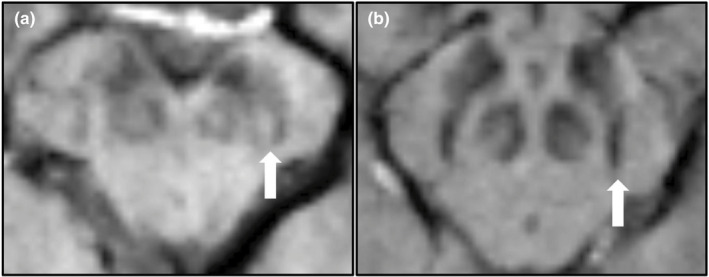
\includegraphics[width=0.8\linewidth]{FileAusiliari/Immagini/degenerative/BRB3-11-e02202-g002}
	\caption{Esempi di segno della coda di rondine (STS) in un individuo malato (a) e di STS assente in un individuo sano (b). Sono mostrate sezioni assiali del mesencefalo mappate tramite imaging pesato con suscettibilità (SWI). Le frecce bianche indicano la diversa configurazione del Nigrosoma-1 (N1). Da Brain Behav. 2021 May 24;11(7):e02202. doi: 10.1002/brb3.2202}
	\label{fig:brb3-11-e02202-g002}
\end{figure*}


La diagnosi differenziale delle sindromi parkinsoniane atipiche beneficia significativamente dell'imaging RM. L'atrofia multisistemica (MSA) evidenzia caratteristica atrofia putaminale, pontica e cerebellare, con ipointensità putaminale T2/SWI e "hot cross bun sign" pontino. La paralisi sopranucleare progressiva (PSP) manifesta atrofia mesencefalica con alterazione del rapporto mesencefalo-ponte, mentre la degenerazione corticobasale (CBD) presenta atrofia frontoparietale asimmetrica con iperintensità della sostanza bianca subcorticale.
Metodiche avanzate quali Diffusion Tensor Imaging (DTI) e risonanza magnetica funzionale (fMRI) consentono la caratterizzazione delle alterazioni microstrutturali della sostanza bianca e delle modificazioni funzionali cerebrali, sebbene la sensibilità nell'identificazione della progressione patologica e nella valutazione della risposta terapeutica necessiti ulteriore validazione. Le limitazioni metodologiche includono variabilità interindividuale e sovrapposizione dei reperti radiologici nelle diverse sindromi parkinsoniane.

\subsection{Trattamento e prognosi}

\subsection{Checklist di refertazione}

\begin{itemize}[label=$\square$] % Riquadro vuoto come simbolo
	\item Escludi altre cause di parkinsonismo (es ictus)
	\item Controlla il segnale dei nigrosomi
	\item Controlla il trofismo delle strutture sottotentoriali
\end{itemize}

\subsection{Bibliografia}
\small{
	
	
}

\note{Nota a margine}
\expl{Nota a margine colorata}
\input{Capitoli/degenerative/approccio.tex}
\input{Capitoli/degenerative/degenerative.tex}
\section{Morbo di Parkinson}

\subsection{Definizione}

\subsection{Eziologia}

\begin{figure*}[h]
	\centering
	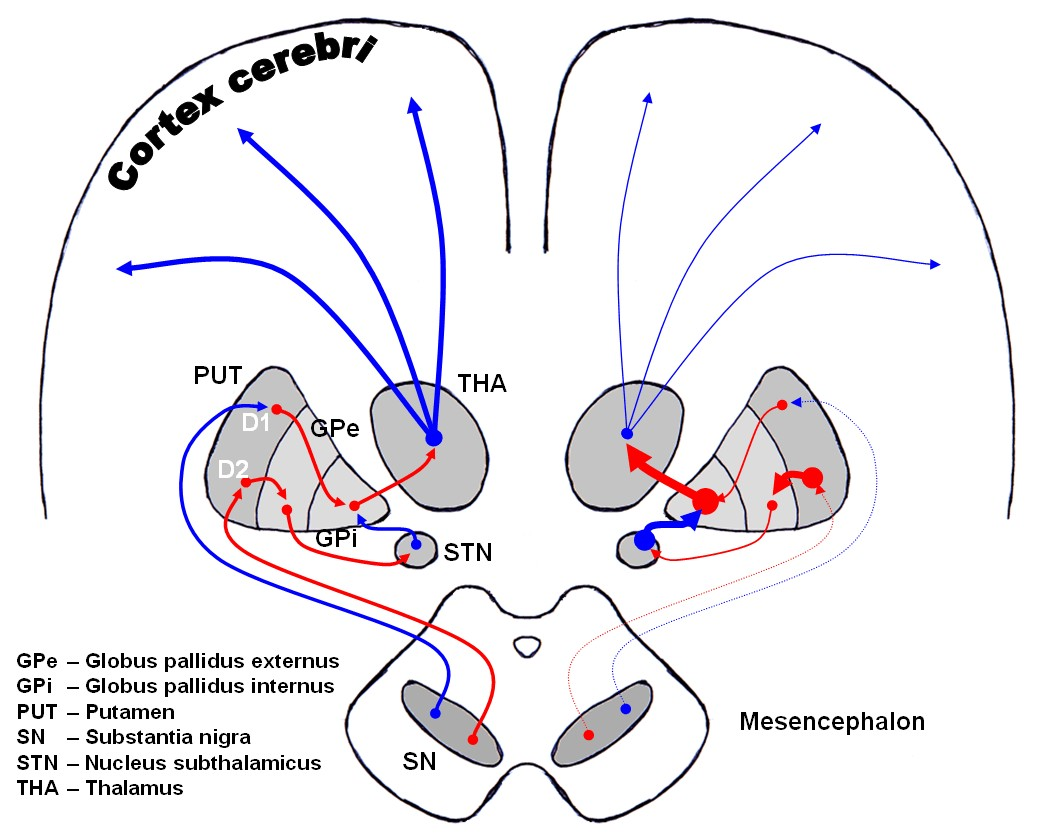
\includegraphics[width=0.5\linewidth]{FileAusiliari/Immagini/degenerative/dopamine-in-parkinsons-disease-illustration}
	\caption[Vie dopaminergiche]{L'immagine mostra le vie dopaminergiche del cervello umano in condizioni normali (a sinistra) e nella malattia di Parkinson (a destra). Le frecce rosse indicano la soppressione del bersaglio, quelle blu la stimolazione della struttura bersaglio. Caso per gentile concessione di Wikipedia, Radiopaedia.org, rID: 36286}
	\label{fig:dopamine-in-parkinsons-disease-illustration}
\end{figure*}

\subsection{Epidemiologia}
Il MP costituisce una delle principali cause di disabilità e mortalità nell'ambito delle patologie neurologiche, con una prevalenza particolarmente elevata negli Stati Uniti e in Canada (160-180 casi/100.000 abitanti). L'incidenza annuale in Nord America oscilla tra 108 e 212 casi ogni 100.000 individui di età $\geq$65 anni, con una prevalenza dello 0,3\% nella popolazione adulta $\geq$40 anni e dell'1,6\% nei soggetti ultrasessantacinquenni.
L'esordio della patologia mostra una significativa correlazione con l'età, manifestandosi tipicamente dalla quinta decade di vita, con un'età media alla diagnosi di 70,5 anni e una finestra di esordio prevalente tra i 45 e i 70 anni. Una variante giovanile può presentarsi tra i 20 e i 40 anni, sebbene l'esordio prima dei 30 anni risulti infrequente. La distribuzione per sesso evidenzia una predominanza maschile, particolarmente accentuata nella fascia d'età 50-60 anni.
L'eziologia del MP comprende fattori di rischio genetici, con particolare rilevanza nelle forme ad esordio precoce, e ambientali, tra cui l'esposizione a pesticidi e inquinanti atmosferici. Sono stati identificati fattori protettivi, inclusi il consumo di caffè, l'attività fisica e il fumo di sigaretta. La patologia si presenta prevalentemente in forma sporadica (85-90\% dei casi), mentre una minoranza dei casi (10-15\%) presenta familiarità positiva.

\subsubsection{Fattori di rischio}
L'eziopatogenesi del Morbo di Parkinson (MP) presenta una complessa interazione di fattori di rischio genetici, ambientali e non modificabili. L'anamnesi familiare positiva per MP in consanguinei di primo grado comporta un incremento del rischio relativo di 2-3 volte. Le forme monogeniche, rappresentanti meno del 10\% della casistica totale, manifestano pattern di ereditarietà autosomica dominante, recessiva o X-linked, caratterizzandosi per un esordio precoce rispetto alle forme sporadiche.
Le mutazioni eterozigoti del gene GBA1 costituiscono un significativo fattore di rischio genetico, unitamente ad alterazioni di altri geni codificanti per enzimi lisosomiali. Il coinvolgimento di geni quali SNCA, LRRK2, VPS35, Parkin, PINK1 e DJ-1 è stato ampiamente documentato. Particolare rilevanza assumono le mutazioni del gene Nurr1, determinante per l'identità neuronale dopaminergica, e del gene DJ-1, cruciale nella risposta allo stress ossidativo. Le alterazioni del gene PINK1, codificante per una chinasi mitocondriale, e del gene Park2, responsabile della sintesi della proteina parkina, sono associate a forme ad esordio precoce.
L'esposizione a neurotossine ambientali, inclusi mercurio, manganese, disolfuro di carbonio, solventi organici, MPTP e monossido di carbonio, può indurre degenerazione nigrostriatale e parkinsonismo. L'uso di neurolettici e l'abuso endovenoso di efedrone possono causare sindromi parkinsoniane potenzialmente irreversibili. Traumi cranici ripetuti, pesticidi, solventi e inquinamento atmosferico rappresentano ulteriori fattori di rischio ambientale documentati.
Tra i fattori non modificabili, l'età avanzata e il sesso maschile emergono come significativi predittori di rischio, con predominanza nella sesta decade di vita. Comorbidità quali depressione, ansia, stipsi, diabete mellito tipo 2, obesità e alterazioni del metabolismo del ferro sono state correlate a un incrementato rischio di MP.
Il consumo di tabacco e caffè, unitamente all'attività fisica regolare, ha mostrato effetti protettivi, sebbene di modesta entità. È fondamentale sottolineare che la maggioranza dei casi di MP rimane idiopatica, suggerendo un'eziologia multifattoriale.

\subsection{Presentazione  clinica}
La sintomatologia del Morbo di Parkinson manifesta un quadro clinico caratterizzato da manifestazioni motorie cardinali e sintomatologia non motoria associata. Il complesso sintomatologico motorio comprende tremore a riposo spesso asimmetrico con frequenza di 4-6 Hz, tipicamente descritto come "pill-rolling", bradicinesia manifestantesi con rallentamento motorio, ipomimia e ridotta oscillazione pendolare degli arti superiori durante la deambulazione, rigidità muscolare ("lead-pipe" o fenomeno della ruota dentata), e instabilità posturale documentabile attraverso il test della retropulsione. La deambulazione risulta caratterizzata da una progressione a piccoli passi con tendenza allo strascicamento e ridotta oscillazione degli arti superiori.
La sintomatologia accessoria include disartria con eloquio esplosivo secondario a incoordinazione linguo-diaframmatica, movimenti involontari della lingua con conseguente difficoltà protrusiva, e incremento della frequenza di ammiccamento palpebrale, quest'ultimo in contrasto con quanto osservato nella corea di Huntington. La disfunzione autonomica, i disturbi olfattivi, la sintomatologia algica, le alterazioni sensitive e i disturbi timici costituiscono il corredo sintomatologico non motorio. Il deterioramento cognitivo, con particolare coinvolgimento delle funzioni attentive, può manifestarsi e progredire nel decorso della patologia.
La progressione temporale della malattia evidenzia un esordio tipicamente unilaterale con successiva bilateralizzazione, manifestandosi prevalentemente nella sesta decade di vita. La responsività alla terapia dopaminergica, in particolare alla levodopa, rappresenta un elemento caratteristico, sebbene il tremore possa risultare farmacoresistente, in contrasto con la significativa risposta della bradicinesia e della rigidità. La variabilità fenotipica interindividuale costituisce un elemento distintivo della patologia.

\subsection{Approccio diagnostico}
L'iter diagnostico della malattia di Parkinson si fonda primariamente sulla valutazione clinica, data l'assenza di biomarcatori patognomonici. La diagnosi richiede la documentazione di bradicinesia associata ad almeno un sintomo cardine tra tremore a riposo o rigidità, valutati mediante la scala MDS-UPDRS standardizzata.
L'approccio diagnostico contempla un'accurata anamnesi ed esame obiettivo neurologico, focalizzati sull'identificazione dei sintomi cardinali: bradicinesia, tremore a riposo (4-6 Hz) tipicamente asimmetrico, rigidità e instabilità posturale. La responsività alla terapia dopaminergica, particolarmente evidente per bradicinesia e rigidità, costituisce un elemento diagnostico supportivo significativo, mentre una mancata risposta a dosaggi adeguati di levodopa suggerisce diagnosi alternative.
L'esclusione di parkinsonismi secondari richiede particolare attenzione all'insorgenza temporale dei sintomi e alla distribuzione topografica del coinvolgimento motorio. La diagnostica per immagini, sebbene non necessaria nelle presentazioni cliniche tipiche con adeguata risposta alla levodopa, può includere RM cerebrale, particolarmente utile mediante sequenze SWI per la valutazione del "swallow tail sign" nigrostriatale. La SPECT con 123I-FP-CIT (DaTscan) documenta la disfunzione dopaminergica presinaptica, mentre la PET con FDG consente la differenziazione metabolica tra PD e sindromi parkinsoniane atipiche.
L'analisi genetica, indicata in casi selezionati (esordio precoce, familiarità positiva, specifiche etnie), e la valutazione autonomica mediante scintigrafia miocardica con MIBG, che evidenzia la denervazione simpatica caratteristica, completano l'iter diagnostico. L'ecografia transcranica può evidenziare l'iperecogenicità della sostanza nera, supportando la diagnosi differenziale.
I criteri MDS stratificano la diagnosi in PD clinicamente stabilita e probabile, bilanciando specificità e sensibilità diagnostica nella pratica clinica.

\begin{Oss}
	La scala MDS-UPDRS (Movement Disorder Society-Unified Parkinson's Disease Rating Scale) è uno strumento di valutazione clinica ampiamente utilizzato per quantificare la gravità dei sintomi motori e non motori della malattia di Parkinson. Questa scala è stata sviluppata per migliorare la consistenza nella valutazione dei sintomi e per integrare meglio gli aspetti non motori della PD.
	Struttura: La scala MDS-UPDRS è composta da quattro sezioni:
	\begin{description}
		\item[Sezione I]{Esperienze non motorie della vita quotidiana. Questa sezione valuta aspetti come le capacità cognitive, i disturbi comportamentali e dell'umore}
		\item [Sezione II]{Esperienze motorie della vita quotidiana. Questa sezione valuta l'impatto dei sintomi motori sulle attività quotidiane}
		\item [Sezione III]{Esame motorio. Questa sezione valuta i segni motori della PD attraverso un esame clinico, come il tremore, la rigidità e la bradicinesia}
		\item[Sezione IV]{Complicanze della terapia. Questa sezione valuta le complicanze associate al trattamento farmacologico}
	\end{description}
	Il punteggio totale per le sezioni I-IV varia da 0 (nessuna disabilità) a 199 (disabilità totale). La sezione III, che valuta i sintomi motori, ha un punteggio che varia da 0 a 132.
	Oltre alla scala MDS-UPDRS, esistono altre scale di valutazione utilizzate nella PD, come la scala di Hoehn e Yahr e la scala di Schwab e England. La scala di Hoehn e Yahr valuta la gravità della malattia da 0 (nessuna malattia) a 5 (paziente costretto su sedia a rotelle o allettato senza assistenza).
\end{Oss}

\subsection{Anatomia patologica}
Dal punto di vista anatomopatologico il morbo di Parkinson si manifesta attraverso inclusioni proteiche intraneuronali denominate corpi di Lewy, costituiti primariamente da aggregati patologici di alfa-sinucleina, una proteina sinaptica fisiologicamente presente nel sistema nervoso centrale. L'accumulo di queste inclusioni, sebbene non patognomonico del morbo di Parkinson essendo documentabile anche nella demenza a corpi di Lewy, rappresenta una caratteristica istopatologica fondamentale quando localizzato nella substantia nigra, in associazione alla perdita neuronale dopaminergica. L'assenza di corpi di Lewy nelle forme post-encefalitiche, caratterizzate invece da grovigli neurofibrillari, e in alcune forme geneticamente determinate, sottolinea l'eterogeneità patogenetica della malattia.
La progressione spazio-temporale della patologia, codificata nello staging di Braak, delinea sei stadi evolutivi caratterizzati da una diffusione ascendente delle alterazioni neuropatologiche. Gli stadi iniziali (1-2) coinvolgono il nucleo motore dorsale dei nervi glossofaringeo e vago e il nucleo olfattivo anteriore, precedendo frequentemente la sintomatologia motoria. Gli stadi intermedi (3-4) documentano il coinvolgimento della substantia nigra pars compacta, del prosencefalo basale e della mesocorteccia temporale, correlando con l'esordio clinico della malattia. Gli stadi terminali (5-6) evidenziano una progressione neocorticale diffusa.
La patogenesi molecolare implica alterazioni del metabolismo dell'alfa-sinucleina, potenzialmente accelerate da disfunzioni delle proteine heat shock o dall'azione della dopamina. Il coinvolgimento della proteina parkin nella degradazione proteasomica evidenzia meccanismi neurodegenerativi potenzialmente indipendenti dalla formazione dei corpi di Lewy.
L'alfa-sinucleina, proteina fisiologicamente localizzata nelle terminazioni presinaptiche neuronali, manifesta nella patogenesi del morbo di Parkinson un processo patologico caratterizzato da misfolding proteico e successiva aggregazione in oligomeri, protofibrille e fibrille, culminante nella formazione dei corpi di Lewy intraneuronali. Questi aggregati proteici, considerati hallmark istopatologico della malattia, evidenziano particolare neurotossicità nella forma protofibrillare, determinando disfunzione e successiva degenerazione neuronale dopaminergica nigrostriatale.
L'identificazione di mutazioni nel gene SNCA, codificante per l'alfa-sinucleina, nelle forme familiari di malattia, unitamente alla documentazione di fenotipi clinici particolarmente aggressivi in presenza di duplicazione o triplicazione genica, ha fornito evidenze significative del ruolo causale di questa proteina nella patogenesi della malattia. La documentata capacità di trasmissione transcellulare dell'alfa-sinucleina patologica costituisce il substrato molecolare della progressione anatomopatologica descritta nello staging di Braak.
La disfunzione sinaptica correlata all'accumulo di alfa-sinucleina rappresenta un meccanismo patogenetico critico, modulato da fattori quali stress ossidativo, alterazioni del sistema ubiquitina-proteasoma e interazione con il metabolismo dopaminergico. Mutazioni nei geni parkin, PINK1 e DJ-1 influenzano il metabolismo dell'alfa-sinucleina attraverso alterazioni dei sistemi di degradazione proteica.
L'alfa-sinucleina costituisce attualmente un promettente target terapeutico, con particolare interesse per lo sviluppo di anticorpi monoclonali specifici e inibitori dell'aggregazione proteica, finalizzati al rallentamento della progressione patologica.

\subsection{Imaging}

\subsubsection{TC}
La TC manifesta un'utilità clinica circoscritta nella valutazione diagnostica primaria del MP, assumendo rilevanza nell'esclusione di patologie strutturali mimiche quali lesioni espansive, idrocefalo o alterazioni vascolari, particolarmente in presenza di presentazioni cliniche atipiche o "red flags" suggestive di diagnosi alternative.
Nel contesto della gestione terapeutica, la TC assume particolare rilevanza nella valutazione post-chirurgica della stimolazione cerebrale profonda (DBS), consentendo la verifica del corretto posizionamento degli elettrodi nel nucleo subtalamico (STN), tipicamente localizzati a 9mm dalla linea mediana, e l'identificazione di eventuali complicanze post-procedurali quali eventi emorragici, ischemici o fenomeni infiammatori transitori, questi ultimi caratterizzati da aree ipodense perilettrodiche a risoluzione graduale. L'utilità della metodica nel follow-up routinario post-DBS risulta secondaria.
La sensibilità subottimale della TC nella diagnosi differenziale tra PD e sindromi parkinsoniane atipiche, incluse atrofia multisistemica e paralisi sopranucleare progressiva, nonché nella distinzione dal tremore essenziale, ne limita significativamente l'applicazione clinica in questo contesto diagnostico.

\subsubsection{RM}
La RM è frequentemente normale nelle sequenze convenzionali (T1, T2, FLAIR) nelle fasi iniziali di malattia. L'implementazione di sequenze susceptibility-weighted imaging (SWI) o T2*-weighted ad alta risoluzione consente la visualizzazione del nigrosoma-1, struttura caratterizzata dal patognomonico "swallow tail sign", la cui perdita correla con la degenerazione dopaminergica nigrostriatale. L'accumulo patologico di ferro nella substantia nigra, quantificabile mediante sequenze SWI/T2* e incrementato del 50\% rispetto ai controlli, costituisce un ulteriore marker diagnostico, complementato dall'imaging della neuromelanina mediante sequenze T1 con impulsi di trasferimento di magnetizzazione (MTC).

\begin{figure*}[h]
	\centering
	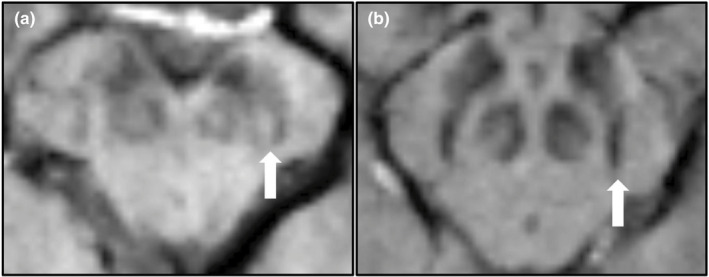
\includegraphics[width=0.8\linewidth]{FileAusiliari/Immagini/degenerative/BRB3-11-e02202-g002}
	\caption{Esempi di segno della coda di rondine (STS) in un individuo malato (a) e di STS assente in un individuo sano (b). Sono mostrate sezioni assiali del mesencefalo mappate tramite imaging pesato con suscettibilità (SWI). Le frecce bianche indicano la diversa configurazione del Nigrosoma-1 (N1). Da Brain Behav. 2021 May 24;11(7):e02202. doi: 10.1002/brb3.2202}
	\label{fig:brb3-11-e02202-g002}
\end{figure*}


La diagnosi differenziale delle sindromi parkinsoniane atipiche beneficia significativamente dell'imaging RM. L'atrofia multisistemica (MSA) evidenzia caratteristica atrofia putaminale, pontica e cerebellare, con ipointensità putaminale T2/SWI e "hot cross bun sign" pontino. La paralisi sopranucleare progressiva (PSP) manifesta atrofia mesencefalica con alterazione del rapporto mesencefalo-ponte, mentre la degenerazione corticobasale (CBD) presenta atrofia frontoparietale asimmetrica con iperintensità della sostanza bianca subcorticale.
Metodiche avanzate quali Diffusion Tensor Imaging (DTI) e risonanza magnetica funzionale (fMRI) consentono la caratterizzazione delle alterazioni microstrutturali della sostanza bianca e delle modificazioni funzionali cerebrali, sebbene la sensibilità nell'identificazione della progressione patologica e nella valutazione della risposta terapeutica necessiti ulteriore validazione. Le limitazioni metodologiche includono variabilità interindividuale e sovrapposizione dei reperti radiologici nelle diverse sindromi parkinsoniane.

\subsection{Trattamento e prognosi}

\subsection{Checklist di refertazione}

\begin{itemize}[label=$\square$] % Riquadro vuoto come simbolo
	\item Escludi altre cause di parkinsonismo (es ictus)
	\item Controlla il segnale dei nigrosomi
	\item Controlla il trofismo delle strutture sottotentoriali
\end{itemize}

\subsection{Bibliografia}
\small{
	
	
}

\note{Nota a margine}
\expl{Nota a margine colorata}
\input{Capitoli/degenerative/approccio.tex}
\input{Capitoli/degenerative/degenerative.tex}
\section{Morbo di Parkinson}

\subsection{Definizione}

\subsection{Eziologia}

\begin{figure*}[h]
	\centering
	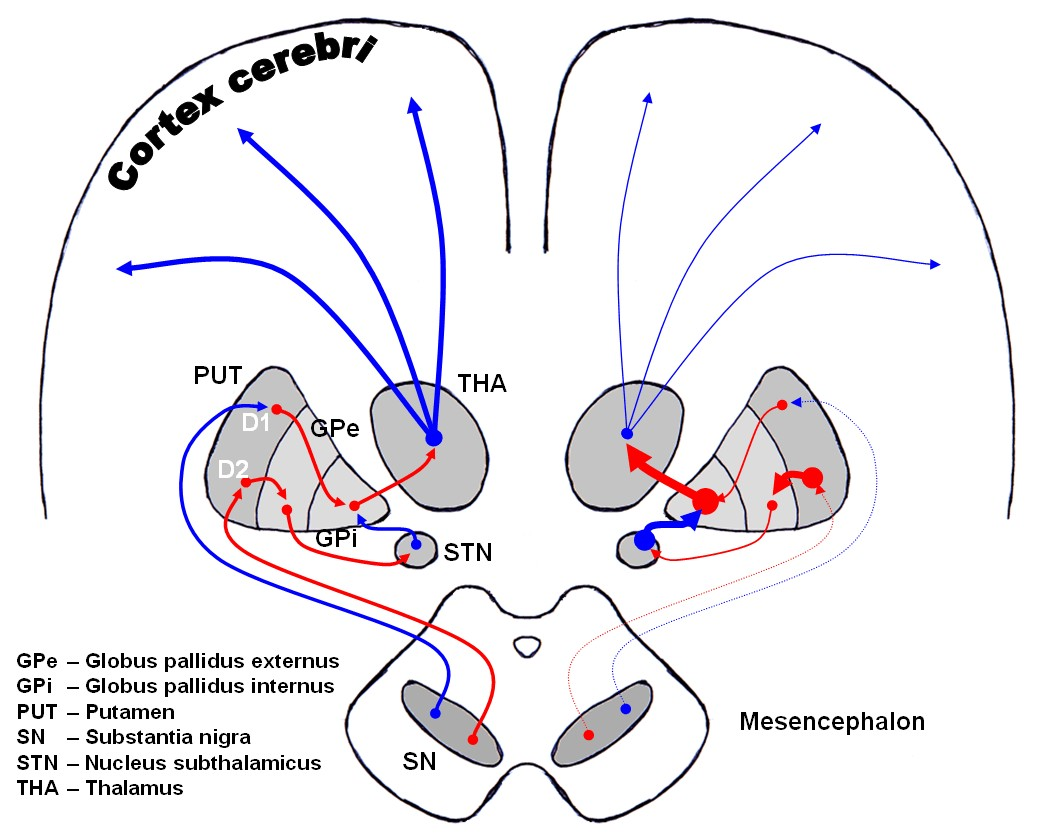
\includegraphics[width=0.5\linewidth]{FileAusiliari/Immagini/degenerative/dopamine-in-parkinsons-disease-illustration}
	\caption[Vie dopaminergiche]{L'immagine mostra le vie dopaminergiche del cervello umano in condizioni normali (a sinistra) e nella malattia di Parkinson (a destra). Le frecce rosse indicano la soppressione del bersaglio, quelle blu la stimolazione della struttura bersaglio. Caso per gentile concessione di Wikipedia, Radiopaedia.org, rID: 36286}
	\label{fig:dopamine-in-parkinsons-disease-illustration}
\end{figure*}

\subsection{Epidemiologia}
Il MP costituisce una delle principali cause di disabilità e mortalità nell'ambito delle patologie neurologiche, con una prevalenza particolarmente elevata negli Stati Uniti e in Canada (160-180 casi/100.000 abitanti). L'incidenza annuale in Nord America oscilla tra 108 e 212 casi ogni 100.000 individui di età $\geq$65 anni, con una prevalenza dello 0,3\% nella popolazione adulta $\geq$40 anni e dell'1,6\% nei soggetti ultrasessantacinquenni.
L'esordio della patologia mostra una significativa correlazione con l'età, manifestandosi tipicamente dalla quinta decade di vita, con un'età media alla diagnosi di 70,5 anni e una finestra di esordio prevalente tra i 45 e i 70 anni. Una variante giovanile può presentarsi tra i 20 e i 40 anni, sebbene l'esordio prima dei 30 anni risulti infrequente. La distribuzione per sesso evidenzia una predominanza maschile, particolarmente accentuata nella fascia d'età 50-60 anni.
L'eziologia del MP comprende fattori di rischio genetici, con particolare rilevanza nelle forme ad esordio precoce, e ambientali, tra cui l'esposizione a pesticidi e inquinanti atmosferici. Sono stati identificati fattori protettivi, inclusi il consumo di caffè, l'attività fisica e il fumo di sigaretta. La patologia si presenta prevalentemente in forma sporadica (85-90\% dei casi), mentre una minoranza dei casi (10-15\%) presenta familiarità positiva.

\subsubsection{Fattori di rischio}
L'eziopatogenesi del Morbo di Parkinson (MP) presenta una complessa interazione di fattori di rischio genetici, ambientali e non modificabili. L'anamnesi familiare positiva per MP in consanguinei di primo grado comporta un incremento del rischio relativo di 2-3 volte. Le forme monogeniche, rappresentanti meno del 10\% della casistica totale, manifestano pattern di ereditarietà autosomica dominante, recessiva o X-linked, caratterizzandosi per un esordio precoce rispetto alle forme sporadiche.
Le mutazioni eterozigoti del gene GBA1 costituiscono un significativo fattore di rischio genetico, unitamente ad alterazioni di altri geni codificanti per enzimi lisosomiali. Il coinvolgimento di geni quali SNCA, LRRK2, VPS35, Parkin, PINK1 e DJ-1 è stato ampiamente documentato. Particolare rilevanza assumono le mutazioni del gene Nurr1, determinante per l'identità neuronale dopaminergica, e del gene DJ-1, cruciale nella risposta allo stress ossidativo. Le alterazioni del gene PINK1, codificante per una chinasi mitocondriale, e del gene Park2, responsabile della sintesi della proteina parkina, sono associate a forme ad esordio precoce.
L'esposizione a neurotossine ambientali, inclusi mercurio, manganese, disolfuro di carbonio, solventi organici, MPTP e monossido di carbonio, può indurre degenerazione nigrostriatale e parkinsonismo. L'uso di neurolettici e l'abuso endovenoso di efedrone possono causare sindromi parkinsoniane potenzialmente irreversibili. Traumi cranici ripetuti, pesticidi, solventi e inquinamento atmosferico rappresentano ulteriori fattori di rischio ambientale documentati.
Tra i fattori non modificabili, l'età avanzata e il sesso maschile emergono come significativi predittori di rischio, con predominanza nella sesta decade di vita. Comorbidità quali depressione, ansia, stipsi, diabete mellito tipo 2, obesità e alterazioni del metabolismo del ferro sono state correlate a un incrementato rischio di MP.
Il consumo di tabacco e caffè, unitamente all'attività fisica regolare, ha mostrato effetti protettivi, sebbene di modesta entità. È fondamentale sottolineare che la maggioranza dei casi di MP rimane idiopatica, suggerendo un'eziologia multifattoriale.

\subsection{Presentazione  clinica}
La sintomatologia del Morbo di Parkinson manifesta un quadro clinico caratterizzato da manifestazioni motorie cardinali e sintomatologia non motoria associata. Il complesso sintomatologico motorio comprende tremore a riposo spesso asimmetrico con frequenza di 4-6 Hz, tipicamente descritto come "pill-rolling", bradicinesia manifestantesi con rallentamento motorio, ipomimia e ridotta oscillazione pendolare degli arti superiori durante la deambulazione, rigidità muscolare ("lead-pipe" o fenomeno della ruota dentata), e instabilità posturale documentabile attraverso il test della retropulsione. La deambulazione risulta caratterizzata da una progressione a piccoli passi con tendenza allo strascicamento e ridotta oscillazione degli arti superiori.
La sintomatologia accessoria include disartria con eloquio esplosivo secondario a incoordinazione linguo-diaframmatica, movimenti involontari della lingua con conseguente difficoltà protrusiva, e incremento della frequenza di ammiccamento palpebrale, quest'ultimo in contrasto con quanto osservato nella corea di Huntington. La disfunzione autonomica, i disturbi olfattivi, la sintomatologia algica, le alterazioni sensitive e i disturbi timici costituiscono il corredo sintomatologico non motorio. Il deterioramento cognitivo, con particolare coinvolgimento delle funzioni attentive, può manifestarsi e progredire nel decorso della patologia.
La progressione temporale della malattia evidenzia un esordio tipicamente unilaterale con successiva bilateralizzazione, manifestandosi prevalentemente nella sesta decade di vita. La responsività alla terapia dopaminergica, in particolare alla levodopa, rappresenta un elemento caratteristico, sebbene il tremore possa risultare farmacoresistente, in contrasto con la significativa risposta della bradicinesia e della rigidità. La variabilità fenotipica interindividuale costituisce un elemento distintivo della patologia.

\subsection{Approccio diagnostico}
L'iter diagnostico della malattia di Parkinson si fonda primariamente sulla valutazione clinica, data l'assenza di biomarcatori patognomonici. La diagnosi richiede la documentazione di bradicinesia associata ad almeno un sintomo cardine tra tremore a riposo o rigidità, valutati mediante la scala MDS-UPDRS standardizzata.
L'approccio diagnostico contempla un'accurata anamnesi ed esame obiettivo neurologico, focalizzati sull'identificazione dei sintomi cardinali: bradicinesia, tremore a riposo (4-6 Hz) tipicamente asimmetrico, rigidità e instabilità posturale. La responsività alla terapia dopaminergica, particolarmente evidente per bradicinesia e rigidità, costituisce un elemento diagnostico supportivo significativo, mentre una mancata risposta a dosaggi adeguati di levodopa suggerisce diagnosi alternative.
L'esclusione di parkinsonismi secondari richiede particolare attenzione all'insorgenza temporale dei sintomi e alla distribuzione topografica del coinvolgimento motorio. La diagnostica per immagini, sebbene non necessaria nelle presentazioni cliniche tipiche con adeguata risposta alla levodopa, può includere RM cerebrale, particolarmente utile mediante sequenze SWI per la valutazione del "swallow tail sign" nigrostriatale. La SPECT con 123I-FP-CIT (DaTscan) documenta la disfunzione dopaminergica presinaptica, mentre la PET con FDG consente la differenziazione metabolica tra PD e sindromi parkinsoniane atipiche.
L'analisi genetica, indicata in casi selezionati (esordio precoce, familiarità positiva, specifiche etnie), e la valutazione autonomica mediante scintigrafia miocardica con MIBG, che evidenzia la denervazione simpatica caratteristica, completano l'iter diagnostico. L'ecografia transcranica può evidenziare l'iperecogenicità della sostanza nera, supportando la diagnosi differenziale.
I criteri MDS stratificano la diagnosi in PD clinicamente stabilita e probabile, bilanciando specificità e sensibilità diagnostica nella pratica clinica.

\begin{Oss}
	La scala MDS-UPDRS (Movement Disorder Society-Unified Parkinson's Disease Rating Scale) è uno strumento di valutazione clinica ampiamente utilizzato per quantificare la gravità dei sintomi motori e non motori della malattia di Parkinson. Questa scala è stata sviluppata per migliorare la consistenza nella valutazione dei sintomi e per integrare meglio gli aspetti non motori della PD.
	Struttura: La scala MDS-UPDRS è composta da quattro sezioni:
	\begin{description}
		\item[Sezione I]{Esperienze non motorie della vita quotidiana. Questa sezione valuta aspetti come le capacità cognitive, i disturbi comportamentali e dell'umore}
		\item [Sezione II]{Esperienze motorie della vita quotidiana. Questa sezione valuta l'impatto dei sintomi motori sulle attività quotidiane}
		\item [Sezione III]{Esame motorio. Questa sezione valuta i segni motori della PD attraverso un esame clinico, come il tremore, la rigidità e la bradicinesia}
		\item[Sezione IV]{Complicanze della terapia. Questa sezione valuta le complicanze associate al trattamento farmacologico}
	\end{description}
	Il punteggio totale per le sezioni I-IV varia da 0 (nessuna disabilità) a 199 (disabilità totale). La sezione III, che valuta i sintomi motori, ha un punteggio che varia da 0 a 132.
	Oltre alla scala MDS-UPDRS, esistono altre scale di valutazione utilizzate nella PD, come la scala di Hoehn e Yahr e la scala di Schwab e England. La scala di Hoehn e Yahr valuta la gravità della malattia da 0 (nessuna malattia) a 5 (paziente costretto su sedia a rotelle o allettato senza assistenza).
\end{Oss}

\subsection{Anatomia patologica}
Dal punto di vista anatomopatologico il morbo di Parkinson si manifesta attraverso inclusioni proteiche intraneuronali denominate corpi di Lewy, costituiti primariamente da aggregati patologici di alfa-sinucleina, una proteina sinaptica fisiologicamente presente nel sistema nervoso centrale. L'accumulo di queste inclusioni, sebbene non patognomonico del morbo di Parkinson essendo documentabile anche nella demenza a corpi di Lewy, rappresenta una caratteristica istopatologica fondamentale quando localizzato nella substantia nigra, in associazione alla perdita neuronale dopaminergica. L'assenza di corpi di Lewy nelle forme post-encefalitiche, caratterizzate invece da grovigli neurofibrillari, e in alcune forme geneticamente determinate, sottolinea l'eterogeneità patogenetica della malattia.
La progressione spazio-temporale della patologia, codificata nello staging di Braak, delinea sei stadi evolutivi caratterizzati da una diffusione ascendente delle alterazioni neuropatologiche. Gli stadi iniziali (1-2) coinvolgono il nucleo motore dorsale dei nervi glossofaringeo e vago e il nucleo olfattivo anteriore, precedendo frequentemente la sintomatologia motoria. Gli stadi intermedi (3-4) documentano il coinvolgimento della substantia nigra pars compacta, del prosencefalo basale e della mesocorteccia temporale, correlando con l'esordio clinico della malattia. Gli stadi terminali (5-6) evidenziano una progressione neocorticale diffusa.
La patogenesi molecolare implica alterazioni del metabolismo dell'alfa-sinucleina, potenzialmente accelerate da disfunzioni delle proteine heat shock o dall'azione della dopamina. Il coinvolgimento della proteina parkin nella degradazione proteasomica evidenzia meccanismi neurodegenerativi potenzialmente indipendenti dalla formazione dei corpi di Lewy.
L'alfa-sinucleina, proteina fisiologicamente localizzata nelle terminazioni presinaptiche neuronali, manifesta nella patogenesi del morbo di Parkinson un processo patologico caratterizzato da misfolding proteico e successiva aggregazione in oligomeri, protofibrille e fibrille, culminante nella formazione dei corpi di Lewy intraneuronali. Questi aggregati proteici, considerati hallmark istopatologico della malattia, evidenziano particolare neurotossicità nella forma protofibrillare, determinando disfunzione e successiva degenerazione neuronale dopaminergica nigrostriatale.
L'identificazione di mutazioni nel gene SNCA, codificante per l'alfa-sinucleina, nelle forme familiari di malattia, unitamente alla documentazione di fenotipi clinici particolarmente aggressivi in presenza di duplicazione o triplicazione genica, ha fornito evidenze significative del ruolo causale di questa proteina nella patogenesi della malattia. La documentata capacità di trasmissione transcellulare dell'alfa-sinucleina patologica costituisce il substrato molecolare della progressione anatomopatologica descritta nello staging di Braak.
La disfunzione sinaptica correlata all'accumulo di alfa-sinucleina rappresenta un meccanismo patogenetico critico, modulato da fattori quali stress ossidativo, alterazioni del sistema ubiquitina-proteasoma e interazione con il metabolismo dopaminergico. Mutazioni nei geni parkin, PINK1 e DJ-1 influenzano il metabolismo dell'alfa-sinucleina attraverso alterazioni dei sistemi di degradazione proteica.
L'alfa-sinucleina costituisce attualmente un promettente target terapeutico, con particolare interesse per lo sviluppo di anticorpi monoclonali specifici e inibitori dell'aggregazione proteica, finalizzati al rallentamento della progressione patologica.

\subsection{Imaging}

\subsubsection{TC}
La TC manifesta un'utilità clinica circoscritta nella valutazione diagnostica primaria del MP, assumendo rilevanza nell'esclusione di patologie strutturali mimiche quali lesioni espansive, idrocefalo o alterazioni vascolari, particolarmente in presenza di presentazioni cliniche atipiche o "red flags" suggestive di diagnosi alternative.
Nel contesto della gestione terapeutica, la TC assume particolare rilevanza nella valutazione post-chirurgica della stimolazione cerebrale profonda (DBS), consentendo la verifica del corretto posizionamento degli elettrodi nel nucleo subtalamico (STN), tipicamente localizzati a 9mm dalla linea mediana, e l'identificazione di eventuali complicanze post-procedurali quali eventi emorragici, ischemici o fenomeni infiammatori transitori, questi ultimi caratterizzati da aree ipodense perilettrodiche a risoluzione graduale. L'utilità della metodica nel follow-up routinario post-DBS risulta secondaria.
La sensibilità subottimale della TC nella diagnosi differenziale tra PD e sindromi parkinsoniane atipiche, incluse atrofia multisistemica e paralisi sopranucleare progressiva, nonché nella distinzione dal tremore essenziale, ne limita significativamente l'applicazione clinica in questo contesto diagnostico.

\subsubsection{RM}
La RM è frequentemente normale nelle sequenze convenzionali (T1, T2, FLAIR) nelle fasi iniziali di malattia. L'implementazione di sequenze susceptibility-weighted imaging (SWI) o T2*-weighted ad alta risoluzione consente la visualizzazione del nigrosoma-1, struttura caratterizzata dal patognomonico "swallow tail sign", la cui perdita correla con la degenerazione dopaminergica nigrostriatale. L'accumulo patologico di ferro nella substantia nigra, quantificabile mediante sequenze SWI/T2* e incrementato del 50\% rispetto ai controlli, costituisce un ulteriore marker diagnostico, complementato dall'imaging della neuromelanina mediante sequenze T1 con impulsi di trasferimento di magnetizzazione (MTC).

\begin{figure*}[h]
	\centering
	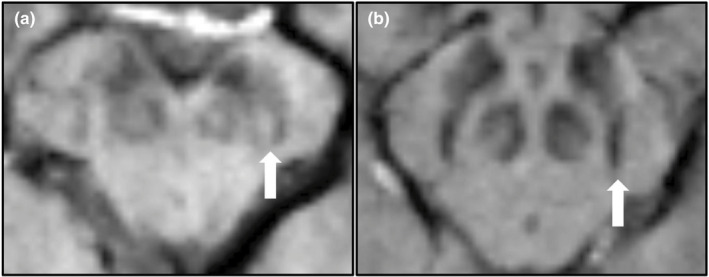
\includegraphics[width=0.8\linewidth]{FileAusiliari/Immagini/degenerative/BRB3-11-e02202-g002}
	\caption{Esempi di segno della coda di rondine (STS) in un individuo malato (a) e di STS assente in un individuo sano (b). Sono mostrate sezioni assiali del mesencefalo mappate tramite imaging pesato con suscettibilità (SWI). Le frecce bianche indicano la diversa configurazione del Nigrosoma-1 (N1). Da Brain Behav. 2021 May 24;11(7):e02202. doi: 10.1002/brb3.2202}
	\label{fig:brb3-11-e02202-g002}
\end{figure*}


La diagnosi differenziale delle sindromi parkinsoniane atipiche beneficia significativamente dell'imaging RM. L'atrofia multisistemica (MSA) evidenzia caratteristica atrofia putaminale, pontica e cerebellare, con ipointensità putaminale T2/SWI e "hot cross bun sign" pontino. La paralisi sopranucleare progressiva (PSP) manifesta atrofia mesencefalica con alterazione del rapporto mesencefalo-ponte, mentre la degenerazione corticobasale (CBD) presenta atrofia frontoparietale asimmetrica con iperintensità della sostanza bianca subcorticale.
Metodiche avanzate quali Diffusion Tensor Imaging (DTI) e risonanza magnetica funzionale (fMRI) consentono la caratterizzazione delle alterazioni microstrutturali della sostanza bianca e delle modificazioni funzionali cerebrali, sebbene la sensibilità nell'identificazione della progressione patologica e nella valutazione della risposta terapeutica necessiti ulteriore validazione. Le limitazioni metodologiche includono variabilità interindividuale e sovrapposizione dei reperti radiologici nelle diverse sindromi parkinsoniane.

\subsection{Trattamento e prognosi}

\subsection{Checklist di refertazione}

\begin{itemize}[label=$\square$] % Riquadro vuoto come simbolo
	\item Escludi altre cause di parkinsonismo (es ictus)
	\item Controlla il segnale dei nigrosomi
	\item Controlla il trofismo delle strutture sottotentoriali
\end{itemize}

\subsection{Bibliografia}
\small{
	
	
}

\note{Nota a margine}
\expl{Nota a margine colorata}
\input{Capitoli/degenerative/approccio.tex}
\input{Capitoli/degenerative/degenerative.tex}
\section{Morbo di Parkinson}

\subsection{Definizione}

\subsection{Eziologia}

\begin{figure*}[h]
	\centering
	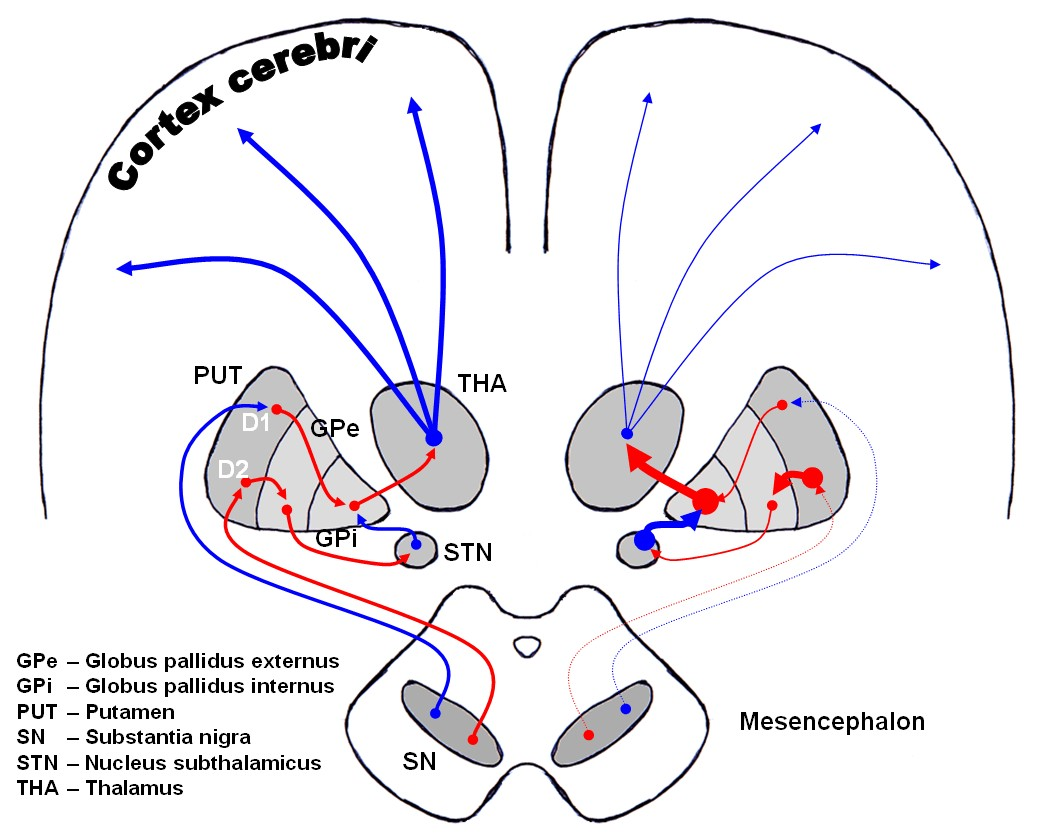
\includegraphics[width=0.5\linewidth]{FileAusiliari/Immagini/degenerative/dopamine-in-parkinsons-disease-illustration}
	\caption[Vie dopaminergiche]{L'immagine mostra le vie dopaminergiche del cervello umano in condizioni normali (a sinistra) e nella malattia di Parkinson (a destra). Le frecce rosse indicano la soppressione del bersaglio, quelle blu la stimolazione della struttura bersaglio. Caso per gentile concessione di Wikipedia, Radiopaedia.org, rID: 36286}
	\label{fig:dopamine-in-parkinsons-disease-illustration}
\end{figure*}

\subsection{Epidemiologia}
Il MP costituisce una delle principali cause di disabilità e mortalità nell'ambito delle patologie neurologiche, con una prevalenza particolarmente elevata negli Stati Uniti e in Canada (160-180 casi/100.000 abitanti). L'incidenza annuale in Nord America oscilla tra 108 e 212 casi ogni 100.000 individui di età $\geq$65 anni, con una prevalenza dello 0,3\% nella popolazione adulta $\geq$40 anni e dell'1,6\% nei soggetti ultrasessantacinquenni.
L'esordio della patologia mostra una significativa correlazione con l'età, manifestandosi tipicamente dalla quinta decade di vita, con un'età media alla diagnosi di 70,5 anni e una finestra di esordio prevalente tra i 45 e i 70 anni. Una variante giovanile può presentarsi tra i 20 e i 40 anni, sebbene l'esordio prima dei 30 anni risulti infrequente. La distribuzione per sesso evidenzia una predominanza maschile, particolarmente accentuata nella fascia d'età 50-60 anni.
L'eziologia del MP comprende fattori di rischio genetici, con particolare rilevanza nelle forme ad esordio precoce, e ambientali, tra cui l'esposizione a pesticidi e inquinanti atmosferici. Sono stati identificati fattori protettivi, inclusi il consumo di caffè, l'attività fisica e il fumo di sigaretta. La patologia si presenta prevalentemente in forma sporadica (85-90\% dei casi), mentre una minoranza dei casi (10-15\%) presenta familiarità positiva.

\subsubsection{Fattori di rischio}
L'eziopatogenesi del Morbo di Parkinson (MP) presenta una complessa interazione di fattori di rischio genetici, ambientali e non modificabili. L'anamnesi familiare positiva per MP in consanguinei di primo grado comporta un incremento del rischio relativo di 2-3 volte. Le forme monogeniche, rappresentanti meno del 10\% della casistica totale, manifestano pattern di ereditarietà autosomica dominante, recessiva o X-linked, caratterizzandosi per un esordio precoce rispetto alle forme sporadiche.
Le mutazioni eterozigoti del gene GBA1 costituiscono un significativo fattore di rischio genetico, unitamente ad alterazioni di altri geni codificanti per enzimi lisosomiali. Il coinvolgimento di geni quali SNCA, LRRK2, VPS35, Parkin, PINK1 e DJ-1 è stato ampiamente documentato. Particolare rilevanza assumono le mutazioni del gene Nurr1, determinante per l'identità neuronale dopaminergica, e del gene DJ-1, cruciale nella risposta allo stress ossidativo. Le alterazioni del gene PINK1, codificante per una chinasi mitocondriale, e del gene Park2, responsabile della sintesi della proteina parkina, sono associate a forme ad esordio precoce.
L'esposizione a neurotossine ambientali, inclusi mercurio, manganese, disolfuro di carbonio, solventi organici, MPTP e monossido di carbonio, può indurre degenerazione nigrostriatale e parkinsonismo. L'uso di neurolettici e l'abuso endovenoso di efedrone possono causare sindromi parkinsoniane potenzialmente irreversibili. Traumi cranici ripetuti, pesticidi, solventi e inquinamento atmosferico rappresentano ulteriori fattori di rischio ambientale documentati.
Tra i fattori non modificabili, l'età avanzata e il sesso maschile emergono come significativi predittori di rischio, con predominanza nella sesta decade di vita. Comorbidità quali depressione, ansia, stipsi, diabete mellito tipo 2, obesità e alterazioni del metabolismo del ferro sono state correlate a un incrementato rischio di MP.
Il consumo di tabacco e caffè, unitamente all'attività fisica regolare, ha mostrato effetti protettivi, sebbene di modesta entità. È fondamentale sottolineare che la maggioranza dei casi di MP rimane idiopatica, suggerendo un'eziologia multifattoriale.

\subsection{Presentazione  clinica}
La sintomatologia del Morbo di Parkinson manifesta un quadro clinico caratterizzato da manifestazioni motorie cardinali e sintomatologia non motoria associata. Il complesso sintomatologico motorio comprende tremore a riposo spesso asimmetrico con frequenza di 4-6 Hz, tipicamente descritto come "pill-rolling", bradicinesia manifestantesi con rallentamento motorio, ipomimia e ridotta oscillazione pendolare degli arti superiori durante la deambulazione, rigidità muscolare ("lead-pipe" o fenomeno della ruota dentata), e instabilità posturale documentabile attraverso il test della retropulsione. La deambulazione risulta caratterizzata da una progressione a piccoli passi con tendenza allo strascicamento e ridotta oscillazione degli arti superiori.
La sintomatologia accessoria include disartria con eloquio esplosivo secondario a incoordinazione linguo-diaframmatica, movimenti involontari della lingua con conseguente difficoltà protrusiva, e incremento della frequenza di ammiccamento palpebrale, quest'ultimo in contrasto con quanto osservato nella corea di Huntington. La disfunzione autonomica, i disturbi olfattivi, la sintomatologia algica, le alterazioni sensitive e i disturbi timici costituiscono il corredo sintomatologico non motorio. Il deterioramento cognitivo, con particolare coinvolgimento delle funzioni attentive, può manifestarsi e progredire nel decorso della patologia.
La progressione temporale della malattia evidenzia un esordio tipicamente unilaterale con successiva bilateralizzazione, manifestandosi prevalentemente nella sesta decade di vita. La responsività alla terapia dopaminergica, in particolare alla levodopa, rappresenta un elemento caratteristico, sebbene il tremore possa risultare farmacoresistente, in contrasto con la significativa risposta della bradicinesia e della rigidità. La variabilità fenotipica interindividuale costituisce un elemento distintivo della patologia.

\subsection{Approccio diagnostico}
L'iter diagnostico della malattia di Parkinson si fonda primariamente sulla valutazione clinica, data l'assenza di biomarcatori patognomonici. La diagnosi richiede la documentazione di bradicinesia associata ad almeno un sintomo cardine tra tremore a riposo o rigidità, valutati mediante la scala MDS-UPDRS standardizzata.
L'approccio diagnostico contempla un'accurata anamnesi ed esame obiettivo neurologico, focalizzati sull'identificazione dei sintomi cardinali: bradicinesia, tremore a riposo (4-6 Hz) tipicamente asimmetrico, rigidità e instabilità posturale. La responsività alla terapia dopaminergica, particolarmente evidente per bradicinesia e rigidità, costituisce un elemento diagnostico supportivo significativo, mentre una mancata risposta a dosaggi adeguati di levodopa suggerisce diagnosi alternative.
L'esclusione di parkinsonismi secondari richiede particolare attenzione all'insorgenza temporale dei sintomi e alla distribuzione topografica del coinvolgimento motorio. La diagnostica per immagini, sebbene non necessaria nelle presentazioni cliniche tipiche con adeguata risposta alla levodopa, può includere RM cerebrale, particolarmente utile mediante sequenze SWI per la valutazione del "swallow tail sign" nigrostriatale. La SPECT con 123I-FP-CIT (DaTscan) documenta la disfunzione dopaminergica presinaptica, mentre la PET con FDG consente la differenziazione metabolica tra PD e sindromi parkinsoniane atipiche.
L'analisi genetica, indicata in casi selezionati (esordio precoce, familiarità positiva, specifiche etnie), e la valutazione autonomica mediante scintigrafia miocardica con MIBG, che evidenzia la denervazione simpatica caratteristica, completano l'iter diagnostico. L'ecografia transcranica può evidenziare l'iperecogenicità della sostanza nera, supportando la diagnosi differenziale.
I criteri MDS stratificano la diagnosi in PD clinicamente stabilita e probabile, bilanciando specificità e sensibilità diagnostica nella pratica clinica.

\begin{Oss}
	La scala MDS-UPDRS (Movement Disorder Society-Unified Parkinson's Disease Rating Scale) è uno strumento di valutazione clinica ampiamente utilizzato per quantificare la gravità dei sintomi motori e non motori della malattia di Parkinson. Questa scala è stata sviluppata per migliorare la consistenza nella valutazione dei sintomi e per integrare meglio gli aspetti non motori della PD.
	Struttura: La scala MDS-UPDRS è composta da quattro sezioni:
	\begin{description}
		\item[Sezione I]{Esperienze non motorie della vita quotidiana. Questa sezione valuta aspetti come le capacità cognitive, i disturbi comportamentali e dell'umore}
		\item [Sezione II]{Esperienze motorie della vita quotidiana. Questa sezione valuta l'impatto dei sintomi motori sulle attività quotidiane}
		\item [Sezione III]{Esame motorio. Questa sezione valuta i segni motori della PD attraverso un esame clinico, come il tremore, la rigidità e la bradicinesia}
		\item[Sezione IV]{Complicanze della terapia. Questa sezione valuta le complicanze associate al trattamento farmacologico}
	\end{description}
	Il punteggio totale per le sezioni I-IV varia da 0 (nessuna disabilità) a 199 (disabilità totale). La sezione III, che valuta i sintomi motori, ha un punteggio che varia da 0 a 132.
	Oltre alla scala MDS-UPDRS, esistono altre scale di valutazione utilizzate nella PD, come la scala di Hoehn e Yahr e la scala di Schwab e England. La scala di Hoehn e Yahr valuta la gravità della malattia da 0 (nessuna malattia) a 5 (paziente costretto su sedia a rotelle o allettato senza assistenza).
\end{Oss}

\subsection{Anatomia patologica}
Dal punto di vista anatomopatologico il morbo di Parkinson si manifesta attraverso inclusioni proteiche intraneuronali denominate corpi di Lewy, costituiti primariamente da aggregati patologici di alfa-sinucleina, una proteina sinaptica fisiologicamente presente nel sistema nervoso centrale. L'accumulo di queste inclusioni, sebbene non patognomonico del morbo di Parkinson essendo documentabile anche nella demenza a corpi di Lewy, rappresenta una caratteristica istopatologica fondamentale quando localizzato nella substantia nigra, in associazione alla perdita neuronale dopaminergica. L'assenza di corpi di Lewy nelle forme post-encefalitiche, caratterizzate invece da grovigli neurofibrillari, e in alcune forme geneticamente determinate, sottolinea l'eterogeneità patogenetica della malattia.
La progressione spazio-temporale della patologia, codificata nello staging di Braak, delinea sei stadi evolutivi caratterizzati da una diffusione ascendente delle alterazioni neuropatologiche. Gli stadi iniziali (1-2) coinvolgono il nucleo motore dorsale dei nervi glossofaringeo e vago e il nucleo olfattivo anteriore, precedendo frequentemente la sintomatologia motoria. Gli stadi intermedi (3-4) documentano il coinvolgimento della substantia nigra pars compacta, del prosencefalo basale e della mesocorteccia temporale, correlando con l'esordio clinico della malattia. Gli stadi terminali (5-6) evidenziano una progressione neocorticale diffusa.
La patogenesi molecolare implica alterazioni del metabolismo dell'alfa-sinucleina, potenzialmente accelerate da disfunzioni delle proteine heat shock o dall'azione della dopamina. Il coinvolgimento della proteina parkin nella degradazione proteasomica evidenzia meccanismi neurodegenerativi potenzialmente indipendenti dalla formazione dei corpi di Lewy.
L'alfa-sinucleina, proteina fisiologicamente localizzata nelle terminazioni presinaptiche neuronali, manifesta nella patogenesi del morbo di Parkinson un processo patologico caratterizzato da misfolding proteico e successiva aggregazione in oligomeri, protofibrille e fibrille, culminante nella formazione dei corpi di Lewy intraneuronali. Questi aggregati proteici, considerati hallmark istopatologico della malattia, evidenziano particolare neurotossicità nella forma protofibrillare, determinando disfunzione e successiva degenerazione neuronale dopaminergica nigrostriatale.
L'identificazione di mutazioni nel gene SNCA, codificante per l'alfa-sinucleina, nelle forme familiari di malattia, unitamente alla documentazione di fenotipi clinici particolarmente aggressivi in presenza di duplicazione o triplicazione genica, ha fornito evidenze significative del ruolo causale di questa proteina nella patogenesi della malattia. La documentata capacità di trasmissione transcellulare dell'alfa-sinucleina patologica costituisce il substrato molecolare della progressione anatomopatologica descritta nello staging di Braak.
La disfunzione sinaptica correlata all'accumulo di alfa-sinucleina rappresenta un meccanismo patogenetico critico, modulato da fattori quali stress ossidativo, alterazioni del sistema ubiquitina-proteasoma e interazione con il metabolismo dopaminergico. Mutazioni nei geni parkin, PINK1 e DJ-1 influenzano il metabolismo dell'alfa-sinucleina attraverso alterazioni dei sistemi di degradazione proteica.
L'alfa-sinucleina costituisce attualmente un promettente target terapeutico, con particolare interesse per lo sviluppo di anticorpi monoclonali specifici e inibitori dell'aggregazione proteica, finalizzati al rallentamento della progressione patologica.

\subsection{Imaging}

\subsubsection{TC}
La TC manifesta un'utilità clinica circoscritta nella valutazione diagnostica primaria del MP, assumendo rilevanza nell'esclusione di patologie strutturali mimiche quali lesioni espansive, idrocefalo o alterazioni vascolari, particolarmente in presenza di presentazioni cliniche atipiche o "red flags" suggestive di diagnosi alternative.
Nel contesto della gestione terapeutica, la TC assume particolare rilevanza nella valutazione post-chirurgica della stimolazione cerebrale profonda (DBS), consentendo la verifica del corretto posizionamento degli elettrodi nel nucleo subtalamico (STN), tipicamente localizzati a 9mm dalla linea mediana, e l'identificazione di eventuali complicanze post-procedurali quali eventi emorragici, ischemici o fenomeni infiammatori transitori, questi ultimi caratterizzati da aree ipodense perilettrodiche a risoluzione graduale. L'utilità della metodica nel follow-up routinario post-DBS risulta secondaria.
La sensibilità subottimale della TC nella diagnosi differenziale tra PD e sindromi parkinsoniane atipiche, incluse atrofia multisistemica e paralisi sopranucleare progressiva, nonché nella distinzione dal tremore essenziale, ne limita significativamente l'applicazione clinica in questo contesto diagnostico.

\subsubsection{RM}
La RM è frequentemente normale nelle sequenze convenzionali (T1, T2, FLAIR) nelle fasi iniziali di malattia. L'implementazione di sequenze susceptibility-weighted imaging (SWI) o T2*-weighted ad alta risoluzione consente la visualizzazione del nigrosoma-1, struttura caratterizzata dal patognomonico "swallow tail sign", la cui perdita correla con la degenerazione dopaminergica nigrostriatale. L'accumulo patologico di ferro nella substantia nigra, quantificabile mediante sequenze SWI/T2* e incrementato del 50\% rispetto ai controlli, costituisce un ulteriore marker diagnostico, complementato dall'imaging della neuromelanina mediante sequenze T1 con impulsi di trasferimento di magnetizzazione (MTC).

\begin{figure*}[h]
	\centering
	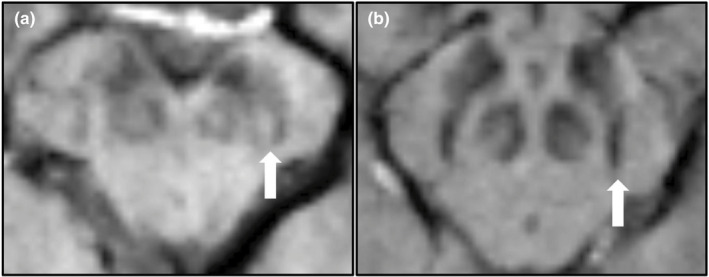
\includegraphics[width=0.8\linewidth]{FileAusiliari/Immagini/degenerative/BRB3-11-e02202-g002}
	\caption{Esempi di segno della coda di rondine (STS) in un individuo malato (a) e di STS assente in un individuo sano (b). Sono mostrate sezioni assiali del mesencefalo mappate tramite imaging pesato con suscettibilità (SWI). Le frecce bianche indicano la diversa configurazione del Nigrosoma-1 (N1). Da Brain Behav. 2021 May 24;11(7):e02202. doi: 10.1002/brb3.2202}
	\label{fig:brb3-11-e02202-g002}
\end{figure*}


La diagnosi differenziale delle sindromi parkinsoniane atipiche beneficia significativamente dell'imaging RM. L'atrofia multisistemica (MSA) evidenzia caratteristica atrofia putaminale, pontica e cerebellare, con ipointensità putaminale T2/SWI e "hot cross bun sign" pontino. La paralisi sopranucleare progressiva (PSP) manifesta atrofia mesencefalica con alterazione del rapporto mesencefalo-ponte, mentre la degenerazione corticobasale (CBD) presenta atrofia frontoparietale asimmetrica con iperintensità della sostanza bianca subcorticale.
Metodiche avanzate quali Diffusion Tensor Imaging (DTI) e risonanza magnetica funzionale (fMRI) consentono la caratterizzazione delle alterazioni microstrutturali della sostanza bianca e delle modificazioni funzionali cerebrali, sebbene la sensibilità nell'identificazione della progressione patologica e nella valutazione della risposta terapeutica necessiti ulteriore validazione. Le limitazioni metodologiche includono variabilità interindividuale e sovrapposizione dei reperti radiologici nelle diverse sindromi parkinsoniane.

\subsection{Trattamento e prognosi}

\subsection{Checklist di refertazione}

\begin{itemize}[label=$\square$] % Riquadro vuoto come simbolo
	\item Escludi altre cause di parkinsonismo (es ictus)
	\item Controlla il segnale dei nigrosomi
	\item Controlla il trofismo delle strutture sottotentoriali
\end{itemize}

\subsection{Bibliografia}
\small{
	
	
}

\note{Nota a margine}
\expl{Nota a margine colorata}
\input{Capitoli/degenerative/approccio.tex}
\input{Capitoli/degenerative/degenerative.tex}
\section{Morbo di Parkinson}

\subsection{Definizione}

\subsection{Eziologia}

\begin{figure*}[h]
	\centering
	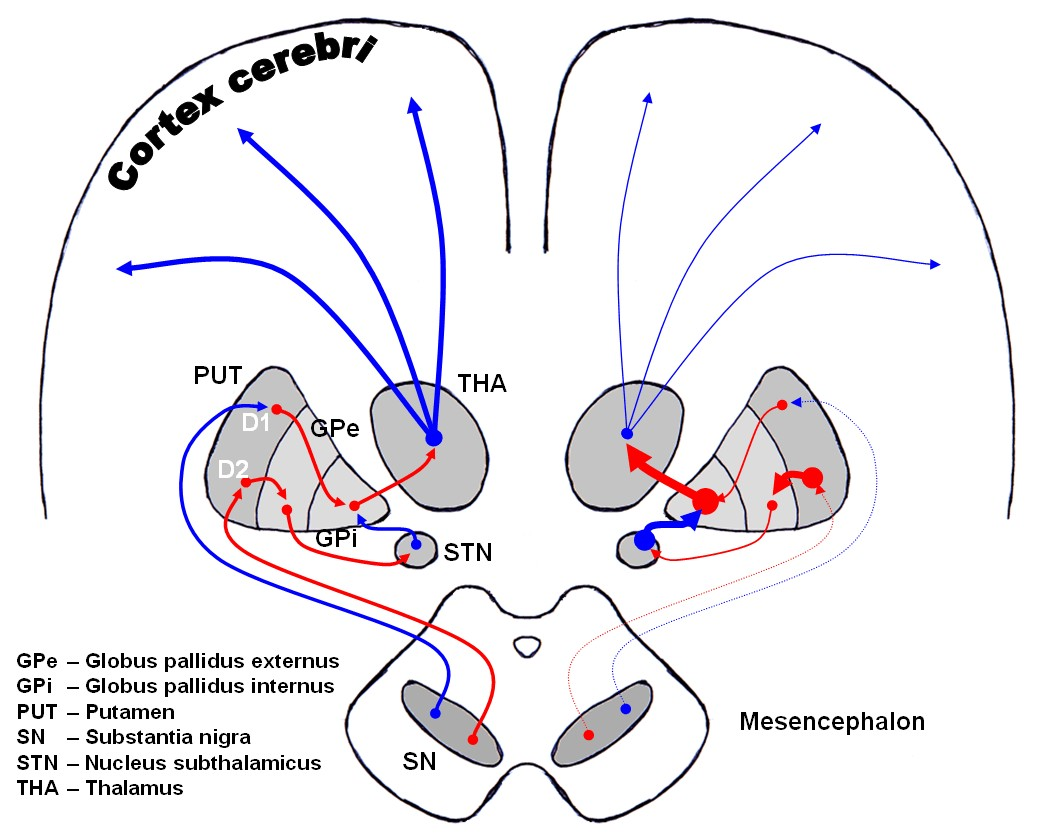
\includegraphics[width=0.5\linewidth]{FileAusiliari/Immagini/degenerative/dopamine-in-parkinsons-disease-illustration}
	\caption[Vie dopaminergiche]{L'immagine mostra le vie dopaminergiche del cervello umano in condizioni normali (a sinistra) e nella malattia di Parkinson (a destra). Le frecce rosse indicano la soppressione del bersaglio, quelle blu la stimolazione della struttura bersaglio. Caso per gentile concessione di Wikipedia, Radiopaedia.org, rID: 36286}
	\label{fig:dopamine-in-parkinsons-disease-illustration}
\end{figure*}

\subsection{Epidemiologia}
Il MP costituisce una delle principali cause di disabilità e mortalità nell'ambito delle patologie neurologiche, con una prevalenza particolarmente elevata negli Stati Uniti e in Canada (160-180 casi/100.000 abitanti). L'incidenza annuale in Nord America oscilla tra 108 e 212 casi ogni 100.000 individui di età $\geq$65 anni, con una prevalenza dello 0,3\% nella popolazione adulta $\geq$40 anni e dell'1,6\% nei soggetti ultrasessantacinquenni.
L'esordio della patologia mostra una significativa correlazione con l'età, manifestandosi tipicamente dalla quinta decade di vita, con un'età media alla diagnosi di 70,5 anni e una finestra di esordio prevalente tra i 45 e i 70 anni. Una variante giovanile può presentarsi tra i 20 e i 40 anni, sebbene l'esordio prima dei 30 anni risulti infrequente. La distribuzione per sesso evidenzia una predominanza maschile, particolarmente accentuata nella fascia d'età 50-60 anni.
L'eziologia del MP comprende fattori di rischio genetici, con particolare rilevanza nelle forme ad esordio precoce, e ambientali, tra cui l'esposizione a pesticidi e inquinanti atmosferici. Sono stati identificati fattori protettivi, inclusi il consumo di caffè, l'attività fisica e il fumo di sigaretta. La patologia si presenta prevalentemente in forma sporadica (85-90\% dei casi), mentre una minoranza dei casi (10-15\%) presenta familiarità positiva.

\subsubsection{Fattori di rischio}
L'eziopatogenesi del Morbo di Parkinson (MP) presenta una complessa interazione di fattori di rischio genetici, ambientali e non modificabili. L'anamnesi familiare positiva per MP in consanguinei di primo grado comporta un incremento del rischio relativo di 2-3 volte. Le forme monogeniche, rappresentanti meno del 10\% della casistica totale, manifestano pattern di ereditarietà autosomica dominante, recessiva o X-linked, caratterizzandosi per un esordio precoce rispetto alle forme sporadiche.
Le mutazioni eterozigoti del gene GBA1 costituiscono un significativo fattore di rischio genetico, unitamente ad alterazioni di altri geni codificanti per enzimi lisosomiali. Il coinvolgimento di geni quali SNCA, LRRK2, VPS35, Parkin, PINK1 e DJ-1 è stato ampiamente documentato. Particolare rilevanza assumono le mutazioni del gene Nurr1, determinante per l'identità neuronale dopaminergica, e del gene DJ-1, cruciale nella risposta allo stress ossidativo. Le alterazioni del gene PINK1, codificante per una chinasi mitocondriale, e del gene Park2, responsabile della sintesi della proteina parkina, sono associate a forme ad esordio precoce.
L'esposizione a neurotossine ambientali, inclusi mercurio, manganese, disolfuro di carbonio, solventi organici, MPTP e monossido di carbonio, può indurre degenerazione nigrostriatale e parkinsonismo. L'uso di neurolettici e l'abuso endovenoso di efedrone possono causare sindromi parkinsoniane potenzialmente irreversibili. Traumi cranici ripetuti, pesticidi, solventi e inquinamento atmosferico rappresentano ulteriori fattori di rischio ambientale documentati.
Tra i fattori non modificabili, l'età avanzata e il sesso maschile emergono come significativi predittori di rischio, con predominanza nella sesta decade di vita. Comorbidità quali depressione, ansia, stipsi, diabete mellito tipo 2, obesità e alterazioni del metabolismo del ferro sono state correlate a un incrementato rischio di MP.
Il consumo di tabacco e caffè, unitamente all'attività fisica regolare, ha mostrato effetti protettivi, sebbene di modesta entità. È fondamentale sottolineare che la maggioranza dei casi di MP rimane idiopatica, suggerendo un'eziologia multifattoriale.

\subsection{Presentazione  clinica}
La sintomatologia del Morbo di Parkinson manifesta un quadro clinico caratterizzato da manifestazioni motorie cardinali e sintomatologia non motoria associata. Il complesso sintomatologico motorio comprende tremore a riposo spesso asimmetrico con frequenza di 4-6 Hz, tipicamente descritto come "pill-rolling", bradicinesia manifestantesi con rallentamento motorio, ipomimia e ridotta oscillazione pendolare degli arti superiori durante la deambulazione, rigidità muscolare ("lead-pipe" o fenomeno della ruota dentata), e instabilità posturale documentabile attraverso il test della retropulsione. La deambulazione risulta caratterizzata da una progressione a piccoli passi con tendenza allo strascicamento e ridotta oscillazione degli arti superiori.
La sintomatologia accessoria include disartria con eloquio esplosivo secondario a incoordinazione linguo-diaframmatica, movimenti involontari della lingua con conseguente difficoltà protrusiva, e incremento della frequenza di ammiccamento palpebrale, quest'ultimo in contrasto con quanto osservato nella corea di Huntington. La disfunzione autonomica, i disturbi olfattivi, la sintomatologia algica, le alterazioni sensitive e i disturbi timici costituiscono il corredo sintomatologico non motorio. Il deterioramento cognitivo, con particolare coinvolgimento delle funzioni attentive, può manifestarsi e progredire nel decorso della patologia.
La progressione temporale della malattia evidenzia un esordio tipicamente unilaterale con successiva bilateralizzazione, manifestandosi prevalentemente nella sesta decade di vita. La responsività alla terapia dopaminergica, in particolare alla levodopa, rappresenta un elemento caratteristico, sebbene il tremore possa risultare farmacoresistente, in contrasto con la significativa risposta della bradicinesia e della rigidità. La variabilità fenotipica interindividuale costituisce un elemento distintivo della patologia.

\subsection{Approccio diagnostico}
L'iter diagnostico della malattia di Parkinson si fonda primariamente sulla valutazione clinica, data l'assenza di biomarcatori patognomonici. La diagnosi richiede la documentazione di bradicinesia associata ad almeno un sintomo cardine tra tremore a riposo o rigidità, valutati mediante la scala MDS-UPDRS standardizzata.
L'approccio diagnostico contempla un'accurata anamnesi ed esame obiettivo neurologico, focalizzati sull'identificazione dei sintomi cardinali: bradicinesia, tremore a riposo (4-6 Hz) tipicamente asimmetrico, rigidità e instabilità posturale. La responsività alla terapia dopaminergica, particolarmente evidente per bradicinesia e rigidità, costituisce un elemento diagnostico supportivo significativo, mentre una mancata risposta a dosaggi adeguati di levodopa suggerisce diagnosi alternative.
L'esclusione di parkinsonismi secondari richiede particolare attenzione all'insorgenza temporale dei sintomi e alla distribuzione topografica del coinvolgimento motorio. La diagnostica per immagini, sebbene non necessaria nelle presentazioni cliniche tipiche con adeguata risposta alla levodopa, può includere RM cerebrale, particolarmente utile mediante sequenze SWI per la valutazione del "swallow tail sign" nigrostriatale. La SPECT con 123I-FP-CIT (DaTscan) documenta la disfunzione dopaminergica presinaptica, mentre la PET con FDG consente la differenziazione metabolica tra PD e sindromi parkinsoniane atipiche.
L'analisi genetica, indicata in casi selezionati (esordio precoce, familiarità positiva, specifiche etnie), e la valutazione autonomica mediante scintigrafia miocardica con MIBG, che evidenzia la denervazione simpatica caratteristica, completano l'iter diagnostico. L'ecografia transcranica può evidenziare l'iperecogenicità della sostanza nera, supportando la diagnosi differenziale.
I criteri MDS stratificano la diagnosi in PD clinicamente stabilita e probabile, bilanciando specificità e sensibilità diagnostica nella pratica clinica.

\begin{Oss}
	La scala MDS-UPDRS (Movement Disorder Society-Unified Parkinson's Disease Rating Scale) è uno strumento di valutazione clinica ampiamente utilizzato per quantificare la gravità dei sintomi motori e non motori della malattia di Parkinson. Questa scala è stata sviluppata per migliorare la consistenza nella valutazione dei sintomi e per integrare meglio gli aspetti non motori della PD.
	Struttura: La scala MDS-UPDRS è composta da quattro sezioni:
	\begin{description}
		\item[Sezione I]{Esperienze non motorie della vita quotidiana. Questa sezione valuta aspetti come le capacità cognitive, i disturbi comportamentali e dell'umore}
		\item [Sezione II]{Esperienze motorie della vita quotidiana. Questa sezione valuta l'impatto dei sintomi motori sulle attività quotidiane}
		\item [Sezione III]{Esame motorio. Questa sezione valuta i segni motori della PD attraverso un esame clinico, come il tremore, la rigidità e la bradicinesia}
		\item[Sezione IV]{Complicanze della terapia. Questa sezione valuta le complicanze associate al trattamento farmacologico}
	\end{description}
	Il punteggio totale per le sezioni I-IV varia da 0 (nessuna disabilità) a 199 (disabilità totale). La sezione III, che valuta i sintomi motori, ha un punteggio che varia da 0 a 132.
	Oltre alla scala MDS-UPDRS, esistono altre scale di valutazione utilizzate nella PD, come la scala di Hoehn e Yahr e la scala di Schwab e England. La scala di Hoehn e Yahr valuta la gravità della malattia da 0 (nessuna malattia) a 5 (paziente costretto su sedia a rotelle o allettato senza assistenza).
\end{Oss}

\subsection{Anatomia patologica}
Dal punto di vista anatomopatologico il morbo di Parkinson si manifesta attraverso inclusioni proteiche intraneuronali denominate corpi di Lewy, costituiti primariamente da aggregati patologici di alfa-sinucleina, una proteina sinaptica fisiologicamente presente nel sistema nervoso centrale. L'accumulo di queste inclusioni, sebbene non patognomonico del morbo di Parkinson essendo documentabile anche nella demenza a corpi di Lewy, rappresenta una caratteristica istopatologica fondamentale quando localizzato nella substantia nigra, in associazione alla perdita neuronale dopaminergica. L'assenza di corpi di Lewy nelle forme post-encefalitiche, caratterizzate invece da grovigli neurofibrillari, e in alcune forme geneticamente determinate, sottolinea l'eterogeneità patogenetica della malattia.
La progressione spazio-temporale della patologia, codificata nello staging di Braak, delinea sei stadi evolutivi caratterizzati da una diffusione ascendente delle alterazioni neuropatologiche. Gli stadi iniziali (1-2) coinvolgono il nucleo motore dorsale dei nervi glossofaringeo e vago e il nucleo olfattivo anteriore, precedendo frequentemente la sintomatologia motoria. Gli stadi intermedi (3-4) documentano il coinvolgimento della substantia nigra pars compacta, del prosencefalo basale e della mesocorteccia temporale, correlando con l'esordio clinico della malattia. Gli stadi terminali (5-6) evidenziano una progressione neocorticale diffusa.
La patogenesi molecolare implica alterazioni del metabolismo dell'alfa-sinucleina, potenzialmente accelerate da disfunzioni delle proteine heat shock o dall'azione della dopamina. Il coinvolgimento della proteina parkin nella degradazione proteasomica evidenzia meccanismi neurodegenerativi potenzialmente indipendenti dalla formazione dei corpi di Lewy.
L'alfa-sinucleina, proteina fisiologicamente localizzata nelle terminazioni presinaptiche neuronali, manifesta nella patogenesi del morbo di Parkinson un processo patologico caratterizzato da misfolding proteico e successiva aggregazione in oligomeri, protofibrille e fibrille, culminante nella formazione dei corpi di Lewy intraneuronali. Questi aggregati proteici, considerati hallmark istopatologico della malattia, evidenziano particolare neurotossicità nella forma protofibrillare, determinando disfunzione e successiva degenerazione neuronale dopaminergica nigrostriatale.
L'identificazione di mutazioni nel gene SNCA, codificante per l'alfa-sinucleina, nelle forme familiari di malattia, unitamente alla documentazione di fenotipi clinici particolarmente aggressivi in presenza di duplicazione o triplicazione genica, ha fornito evidenze significative del ruolo causale di questa proteina nella patogenesi della malattia. La documentata capacità di trasmissione transcellulare dell'alfa-sinucleina patologica costituisce il substrato molecolare della progressione anatomopatologica descritta nello staging di Braak.
La disfunzione sinaptica correlata all'accumulo di alfa-sinucleina rappresenta un meccanismo patogenetico critico, modulato da fattori quali stress ossidativo, alterazioni del sistema ubiquitina-proteasoma e interazione con il metabolismo dopaminergico. Mutazioni nei geni parkin, PINK1 e DJ-1 influenzano il metabolismo dell'alfa-sinucleina attraverso alterazioni dei sistemi di degradazione proteica.
L'alfa-sinucleina costituisce attualmente un promettente target terapeutico, con particolare interesse per lo sviluppo di anticorpi monoclonali specifici e inibitori dell'aggregazione proteica, finalizzati al rallentamento della progressione patologica.

\subsection{Imaging}

\subsubsection{TC}
La TC manifesta un'utilità clinica circoscritta nella valutazione diagnostica primaria del MP, assumendo rilevanza nell'esclusione di patologie strutturali mimiche quali lesioni espansive, idrocefalo o alterazioni vascolari, particolarmente in presenza di presentazioni cliniche atipiche o "red flags" suggestive di diagnosi alternative.
Nel contesto della gestione terapeutica, la TC assume particolare rilevanza nella valutazione post-chirurgica della stimolazione cerebrale profonda (DBS), consentendo la verifica del corretto posizionamento degli elettrodi nel nucleo subtalamico (STN), tipicamente localizzati a 9mm dalla linea mediana, e l'identificazione di eventuali complicanze post-procedurali quali eventi emorragici, ischemici o fenomeni infiammatori transitori, questi ultimi caratterizzati da aree ipodense perilettrodiche a risoluzione graduale. L'utilità della metodica nel follow-up routinario post-DBS risulta secondaria.
La sensibilità subottimale della TC nella diagnosi differenziale tra PD e sindromi parkinsoniane atipiche, incluse atrofia multisistemica e paralisi sopranucleare progressiva, nonché nella distinzione dal tremore essenziale, ne limita significativamente l'applicazione clinica in questo contesto diagnostico.

\subsubsection{RM}
La RM è frequentemente normale nelle sequenze convenzionali (T1, T2, FLAIR) nelle fasi iniziali di malattia. L'implementazione di sequenze susceptibility-weighted imaging (SWI) o T2*-weighted ad alta risoluzione consente la visualizzazione del nigrosoma-1, struttura caratterizzata dal patognomonico "swallow tail sign", la cui perdita correla con la degenerazione dopaminergica nigrostriatale. L'accumulo patologico di ferro nella substantia nigra, quantificabile mediante sequenze SWI/T2* e incrementato del 50\% rispetto ai controlli, costituisce un ulteriore marker diagnostico, complementato dall'imaging della neuromelanina mediante sequenze T1 con impulsi di trasferimento di magnetizzazione (MTC).

\begin{figure*}[h]
	\centering
	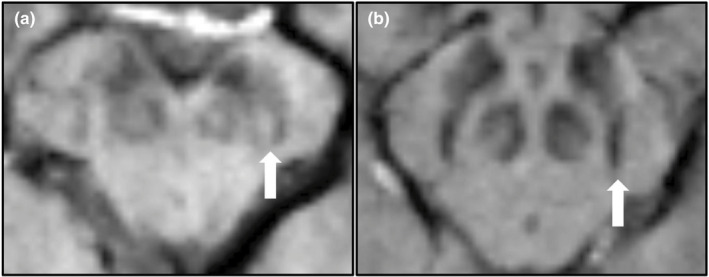
\includegraphics[width=0.8\linewidth]{FileAusiliari/Immagini/degenerative/BRB3-11-e02202-g002}
	\caption{Esempi di segno della coda di rondine (STS) in un individuo malato (a) e di STS assente in un individuo sano (b). Sono mostrate sezioni assiali del mesencefalo mappate tramite imaging pesato con suscettibilità (SWI). Le frecce bianche indicano la diversa configurazione del Nigrosoma-1 (N1). Da Brain Behav. 2021 May 24;11(7):e02202. doi: 10.1002/brb3.2202}
	\label{fig:brb3-11-e02202-g002}
\end{figure*}


La diagnosi differenziale delle sindromi parkinsoniane atipiche beneficia significativamente dell'imaging RM. L'atrofia multisistemica (MSA) evidenzia caratteristica atrofia putaminale, pontica e cerebellare, con ipointensità putaminale T2/SWI e "hot cross bun sign" pontino. La paralisi sopranucleare progressiva (PSP) manifesta atrofia mesencefalica con alterazione del rapporto mesencefalo-ponte, mentre la degenerazione corticobasale (CBD) presenta atrofia frontoparietale asimmetrica con iperintensità della sostanza bianca subcorticale.
Metodiche avanzate quali Diffusion Tensor Imaging (DTI) e risonanza magnetica funzionale (fMRI) consentono la caratterizzazione delle alterazioni microstrutturali della sostanza bianca e delle modificazioni funzionali cerebrali, sebbene la sensibilità nell'identificazione della progressione patologica e nella valutazione della risposta terapeutica necessiti ulteriore validazione. Le limitazioni metodologiche includono variabilità interindividuale e sovrapposizione dei reperti radiologici nelle diverse sindromi parkinsoniane.

\subsection{Trattamento e prognosi}

\subsection{Checklist di refertazione}

\begin{itemize}[label=$\square$] % Riquadro vuoto come simbolo
	\item Escludi altre cause di parkinsonismo (es ictus)
	\item Controlla il segnale dei nigrosomi
	\item Controlla il trofismo delle strutture sottotentoriali
\end{itemize}

\subsection{Bibliografia}
\small{
	
	
}

\note{Nota a margine}
\expl{Nota a margine colorata}
\input{Capitoli/degenerative/approccio.tex}
\input{Capitoli/degenerative/degenerative.tex}
\section{Morbo di Parkinson}

\subsection{Definizione}

\subsection{Eziologia}

\begin{figure*}[h]
	\centering
	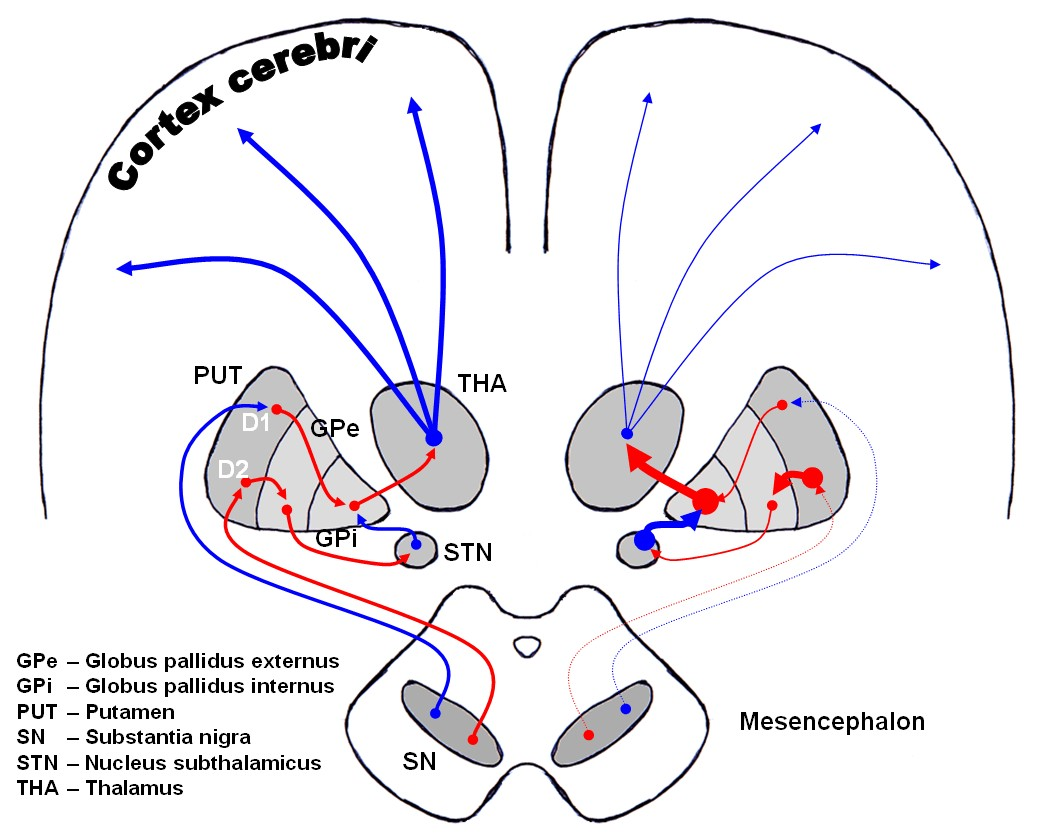
\includegraphics[width=0.5\linewidth]{FileAusiliari/Immagini/degenerative/dopamine-in-parkinsons-disease-illustration}
	\caption[Vie dopaminergiche]{L'immagine mostra le vie dopaminergiche del cervello umano in condizioni normali (a sinistra) e nella malattia di Parkinson (a destra). Le frecce rosse indicano la soppressione del bersaglio, quelle blu la stimolazione della struttura bersaglio. Caso per gentile concessione di Wikipedia, Radiopaedia.org, rID: 36286}
	\label{fig:dopamine-in-parkinsons-disease-illustration}
\end{figure*}

\subsection{Epidemiologia}
Il MP costituisce una delle principali cause di disabilità e mortalità nell'ambito delle patologie neurologiche, con una prevalenza particolarmente elevata negli Stati Uniti e in Canada (160-180 casi/100.000 abitanti). L'incidenza annuale in Nord America oscilla tra 108 e 212 casi ogni 100.000 individui di età $\geq$65 anni, con una prevalenza dello 0,3\% nella popolazione adulta $\geq$40 anni e dell'1,6\% nei soggetti ultrasessantacinquenni.
L'esordio della patologia mostra una significativa correlazione con l'età, manifestandosi tipicamente dalla quinta decade di vita, con un'età media alla diagnosi di 70,5 anni e una finestra di esordio prevalente tra i 45 e i 70 anni. Una variante giovanile può presentarsi tra i 20 e i 40 anni, sebbene l'esordio prima dei 30 anni risulti infrequente. La distribuzione per sesso evidenzia una predominanza maschile, particolarmente accentuata nella fascia d'età 50-60 anni.
L'eziologia del MP comprende fattori di rischio genetici, con particolare rilevanza nelle forme ad esordio precoce, e ambientali, tra cui l'esposizione a pesticidi e inquinanti atmosferici. Sono stati identificati fattori protettivi, inclusi il consumo di caffè, l'attività fisica e il fumo di sigaretta. La patologia si presenta prevalentemente in forma sporadica (85-90\% dei casi), mentre una minoranza dei casi (10-15\%) presenta familiarità positiva.

\subsubsection{Fattori di rischio}
L'eziopatogenesi del Morbo di Parkinson (MP) presenta una complessa interazione di fattori di rischio genetici, ambientali e non modificabili. L'anamnesi familiare positiva per MP in consanguinei di primo grado comporta un incremento del rischio relativo di 2-3 volte. Le forme monogeniche, rappresentanti meno del 10\% della casistica totale, manifestano pattern di ereditarietà autosomica dominante, recessiva o X-linked, caratterizzandosi per un esordio precoce rispetto alle forme sporadiche.
Le mutazioni eterozigoti del gene GBA1 costituiscono un significativo fattore di rischio genetico, unitamente ad alterazioni di altri geni codificanti per enzimi lisosomiali. Il coinvolgimento di geni quali SNCA, LRRK2, VPS35, Parkin, PINK1 e DJ-1 è stato ampiamente documentato. Particolare rilevanza assumono le mutazioni del gene Nurr1, determinante per l'identità neuronale dopaminergica, e del gene DJ-1, cruciale nella risposta allo stress ossidativo. Le alterazioni del gene PINK1, codificante per una chinasi mitocondriale, e del gene Park2, responsabile della sintesi della proteina parkina, sono associate a forme ad esordio precoce.
L'esposizione a neurotossine ambientali, inclusi mercurio, manganese, disolfuro di carbonio, solventi organici, MPTP e monossido di carbonio, può indurre degenerazione nigrostriatale e parkinsonismo. L'uso di neurolettici e l'abuso endovenoso di efedrone possono causare sindromi parkinsoniane potenzialmente irreversibili. Traumi cranici ripetuti, pesticidi, solventi e inquinamento atmosferico rappresentano ulteriori fattori di rischio ambientale documentati.
Tra i fattori non modificabili, l'età avanzata e il sesso maschile emergono come significativi predittori di rischio, con predominanza nella sesta decade di vita. Comorbidità quali depressione, ansia, stipsi, diabete mellito tipo 2, obesità e alterazioni del metabolismo del ferro sono state correlate a un incrementato rischio di MP.
Il consumo di tabacco e caffè, unitamente all'attività fisica regolare, ha mostrato effetti protettivi, sebbene di modesta entità. È fondamentale sottolineare che la maggioranza dei casi di MP rimane idiopatica, suggerendo un'eziologia multifattoriale.

\subsection{Presentazione  clinica}
La sintomatologia del Morbo di Parkinson manifesta un quadro clinico caratterizzato da manifestazioni motorie cardinali e sintomatologia non motoria associata. Il complesso sintomatologico motorio comprende tremore a riposo spesso asimmetrico con frequenza di 4-6 Hz, tipicamente descritto come "pill-rolling", bradicinesia manifestantesi con rallentamento motorio, ipomimia e ridotta oscillazione pendolare degli arti superiori durante la deambulazione, rigidità muscolare ("lead-pipe" o fenomeno della ruota dentata), e instabilità posturale documentabile attraverso il test della retropulsione. La deambulazione risulta caratterizzata da una progressione a piccoli passi con tendenza allo strascicamento e ridotta oscillazione degli arti superiori.
La sintomatologia accessoria include disartria con eloquio esplosivo secondario a incoordinazione linguo-diaframmatica, movimenti involontari della lingua con conseguente difficoltà protrusiva, e incremento della frequenza di ammiccamento palpebrale, quest'ultimo in contrasto con quanto osservato nella corea di Huntington. La disfunzione autonomica, i disturbi olfattivi, la sintomatologia algica, le alterazioni sensitive e i disturbi timici costituiscono il corredo sintomatologico non motorio. Il deterioramento cognitivo, con particolare coinvolgimento delle funzioni attentive, può manifestarsi e progredire nel decorso della patologia.
La progressione temporale della malattia evidenzia un esordio tipicamente unilaterale con successiva bilateralizzazione, manifestandosi prevalentemente nella sesta decade di vita. La responsività alla terapia dopaminergica, in particolare alla levodopa, rappresenta un elemento caratteristico, sebbene il tremore possa risultare farmacoresistente, in contrasto con la significativa risposta della bradicinesia e della rigidità. La variabilità fenotipica interindividuale costituisce un elemento distintivo della patologia.

\subsection{Approccio diagnostico}
L'iter diagnostico della malattia di Parkinson si fonda primariamente sulla valutazione clinica, data l'assenza di biomarcatori patognomonici. La diagnosi richiede la documentazione di bradicinesia associata ad almeno un sintomo cardine tra tremore a riposo o rigidità, valutati mediante la scala MDS-UPDRS standardizzata.
L'approccio diagnostico contempla un'accurata anamnesi ed esame obiettivo neurologico, focalizzati sull'identificazione dei sintomi cardinali: bradicinesia, tremore a riposo (4-6 Hz) tipicamente asimmetrico, rigidità e instabilità posturale. La responsività alla terapia dopaminergica, particolarmente evidente per bradicinesia e rigidità, costituisce un elemento diagnostico supportivo significativo, mentre una mancata risposta a dosaggi adeguati di levodopa suggerisce diagnosi alternative.
L'esclusione di parkinsonismi secondari richiede particolare attenzione all'insorgenza temporale dei sintomi e alla distribuzione topografica del coinvolgimento motorio. La diagnostica per immagini, sebbene non necessaria nelle presentazioni cliniche tipiche con adeguata risposta alla levodopa, può includere RM cerebrale, particolarmente utile mediante sequenze SWI per la valutazione del "swallow tail sign" nigrostriatale. La SPECT con 123I-FP-CIT (DaTscan) documenta la disfunzione dopaminergica presinaptica, mentre la PET con FDG consente la differenziazione metabolica tra PD e sindromi parkinsoniane atipiche.
L'analisi genetica, indicata in casi selezionati (esordio precoce, familiarità positiva, specifiche etnie), e la valutazione autonomica mediante scintigrafia miocardica con MIBG, che evidenzia la denervazione simpatica caratteristica, completano l'iter diagnostico. L'ecografia transcranica può evidenziare l'iperecogenicità della sostanza nera, supportando la diagnosi differenziale.
I criteri MDS stratificano la diagnosi in PD clinicamente stabilita e probabile, bilanciando specificità e sensibilità diagnostica nella pratica clinica.

\begin{Oss}
	La scala MDS-UPDRS (Movement Disorder Society-Unified Parkinson's Disease Rating Scale) è uno strumento di valutazione clinica ampiamente utilizzato per quantificare la gravità dei sintomi motori e non motori della malattia di Parkinson. Questa scala è stata sviluppata per migliorare la consistenza nella valutazione dei sintomi e per integrare meglio gli aspetti non motori della PD.
	Struttura: La scala MDS-UPDRS è composta da quattro sezioni:
	\begin{description}
		\item[Sezione I]{Esperienze non motorie della vita quotidiana. Questa sezione valuta aspetti come le capacità cognitive, i disturbi comportamentali e dell'umore}
		\item [Sezione II]{Esperienze motorie della vita quotidiana. Questa sezione valuta l'impatto dei sintomi motori sulle attività quotidiane}
		\item [Sezione III]{Esame motorio. Questa sezione valuta i segni motori della PD attraverso un esame clinico, come il tremore, la rigidità e la bradicinesia}
		\item[Sezione IV]{Complicanze della terapia. Questa sezione valuta le complicanze associate al trattamento farmacologico}
	\end{description}
	Il punteggio totale per le sezioni I-IV varia da 0 (nessuna disabilità) a 199 (disabilità totale). La sezione III, che valuta i sintomi motori, ha un punteggio che varia da 0 a 132.
	Oltre alla scala MDS-UPDRS, esistono altre scale di valutazione utilizzate nella PD, come la scala di Hoehn e Yahr e la scala di Schwab e England. La scala di Hoehn e Yahr valuta la gravità della malattia da 0 (nessuna malattia) a 5 (paziente costretto su sedia a rotelle o allettato senza assistenza).
\end{Oss}

\subsection{Anatomia patologica}
Dal punto di vista anatomopatologico il morbo di Parkinson si manifesta attraverso inclusioni proteiche intraneuronali denominate corpi di Lewy, costituiti primariamente da aggregati patologici di alfa-sinucleina, una proteina sinaptica fisiologicamente presente nel sistema nervoso centrale. L'accumulo di queste inclusioni, sebbene non patognomonico del morbo di Parkinson essendo documentabile anche nella demenza a corpi di Lewy, rappresenta una caratteristica istopatologica fondamentale quando localizzato nella substantia nigra, in associazione alla perdita neuronale dopaminergica. L'assenza di corpi di Lewy nelle forme post-encefalitiche, caratterizzate invece da grovigli neurofibrillari, e in alcune forme geneticamente determinate, sottolinea l'eterogeneità patogenetica della malattia.
La progressione spazio-temporale della patologia, codificata nello staging di Braak, delinea sei stadi evolutivi caratterizzati da una diffusione ascendente delle alterazioni neuropatologiche. Gli stadi iniziali (1-2) coinvolgono il nucleo motore dorsale dei nervi glossofaringeo e vago e il nucleo olfattivo anteriore, precedendo frequentemente la sintomatologia motoria. Gli stadi intermedi (3-4) documentano il coinvolgimento della substantia nigra pars compacta, del prosencefalo basale e della mesocorteccia temporale, correlando con l'esordio clinico della malattia. Gli stadi terminali (5-6) evidenziano una progressione neocorticale diffusa.
La patogenesi molecolare implica alterazioni del metabolismo dell'alfa-sinucleina, potenzialmente accelerate da disfunzioni delle proteine heat shock o dall'azione della dopamina. Il coinvolgimento della proteina parkin nella degradazione proteasomica evidenzia meccanismi neurodegenerativi potenzialmente indipendenti dalla formazione dei corpi di Lewy.
L'alfa-sinucleina, proteina fisiologicamente localizzata nelle terminazioni presinaptiche neuronali, manifesta nella patogenesi del morbo di Parkinson un processo patologico caratterizzato da misfolding proteico e successiva aggregazione in oligomeri, protofibrille e fibrille, culminante nella formazione dei corpi di Lewy intraneuronali. Questi aggregati proteici, considerati hallmark istopatologico della malattia, evidenziano particolare neurotossicità nella forma protofibrillare, determinando disfunzione e successiva degenerazione neuronale dopaminergica nigrostriatale.
L'identificazione di mutazioni nel gene SNCA, codificante per l'alfa-sinucleina, nelle forme familiari di malattia, unitamente alla documentazione di fenotipi clinici particolarmente aggressivi in presenza di duplicazione o triplicazione genica, ha fornito evidenze significative del ruolo causale di questa proteina nella patogenesi della malattia. La documentata capacità di trasmissione transcellulare dell'alfa-sinucleina patologica costituisce il substrato molecolare della progressione anatomopatologica descritta nello staging di Braak.
La disfunzione sinaptica correlata all'accumulo di alfa-sinucleina rappresenta un meccanismo patogenetico critico, modulato da fattori quali stress ossidativo, alterazioni del sistema ubiquitina-proteasoma e interazione con il metabolismo dopaminergico. Mutazioni nei geni parkin, PINK1 e DJ-1 influenzano il metabolismo dell'alfa-sinucleina attraverso alterazioni dei sistemi di degradazione proteica.
L'alfa-sinucleina costituisce attualmente un promettente target terapeutico, con particolare interesse per lo sviluppo di anticorpi monoclonali specifici e inibitori dell'aggregazione proteica, finalizzati al rallentamento della progressione patologica.

\subsection{Imaging}

\subsubsection{TC}
La TC manifesta un'utilità clinica circoscritta nella valutazione diagnostica primaria del MP, assumendo rilevanza nell'esclusione di patologie strutturali mimiche quali lesioni espansive, idrocefalo o alterazioni vascolari, particolarmente in presenza di presentazioni cliniche atipiche o "red flags" suggestive di diagnosi alternative.
Nel contesto della gestione terapeutica, la TC assume particolare rilevanza nella valutazione post-chirurgica della stimolazione cerebrale profonda (DBS), consentendo la verifica del corretto posizionamento degli elettrodi nel nucleo subtalamico (STN), tipicamente localizzati a 9mm dalla linea mediana, e l'identificazione di eventuali complicanze post-procedurali quali eventi emorragici, ischemici o fenomeni infiammatori transitori, questi ultimi caratterizzati da aree ipodense perilettrodiche a risoluzione graduale. L'utilità della metodica nel follow-up routinario post-DBS risulta secondaria.
La sensibilità subottimale della TC nella diagnosi differenziale tra PD e sindromi parkinsoniane atipiche, incluse atrofia multisistemica e paralisi sopranucleare progressiva, nonché nella distinzione dal tremore essenziale, ne limita significativamente l'applicazione clinica in questo contesto diagnostico.

\subsubsection{RM}
La RM è frequentemente normale nelle sequenze convenzionali (T1, T2, FLAIR) nelle fasi iniziali di malattia. L'implementazione di sequenze susceptibility-weighted imaging (SWI) o T2*-weighted ad alta risoluzione consente la visualizzazione del nigrosoma-1, struttura caratterizzata dal patognomonico "swallow tail sign", la cui perdita correla con la degenerazione dopaminergica nigrostriatale. L'accumulo patologico di ferro nella substantia nigra, quantificabile mediante sequenze SWI/T2* e incrementato del 50\% rispetto ai controlli, costituisce un ulteriore marker diagnostico, complementato dall'imaging della neuromelanina mediante sequenze T1 con impulsi di trasferimento di magnetizzazione (MTC).

\begin{figure*}[h]
	\centering
	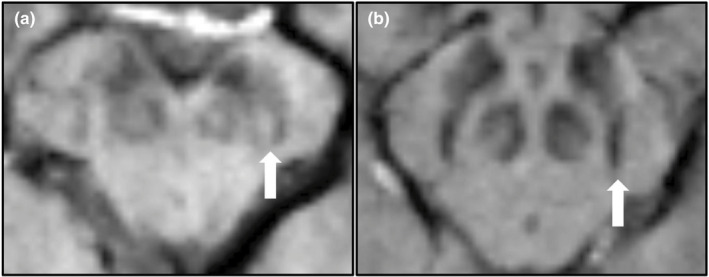
\includegraphics[width=0.8\linewidth]{FileAusiliari/Immagini/degenerative/BRB3-11-e02202-g002}
	\caption{Esempi di segno della coda di rondine (STS) in un individuo malato (a) e di STS assente in un individuo sano (b). Sono mostrate sezioni assiali del mesencefalo mappate tramite imaging pesato con suscettibilità (SWI). Le frecce bianche indicano la diversa configurazione del Nigrosoma-1 (N1). Da Brain Behav. 2021 May 24;11(7):e02202. doi: 10.1002/brb3.2202}
	\label{fig:brb3-11-e02202-g002}
\end{figure*}


La diagnosi differenziale delle sindromi parkinsoniane atipiche beneficia significativamente dell'imaging RM. L'atrofia multisistemica (MSA) evidenzia caratteristica atrofia putaminale, pontica e cerebellare, con ipointensità putaminale T2/SWI e "hot cross bun sign" pontino. La paralisi sopranucleare progressiva (PSP) manifesta atrofia mesencefalica con alterazione del rapporto mesencefalo-ponte, mentre la degenerazione corticobasale (CBD) presenta atrofia frontoparietale asimmetrica con iperintensità della sostanza bianca subcorticale.
Metodiche avanzate quali Diffusion Tensor Imaging (DTI) e risonanza magnetica funzionale (fMRI) consentono la caratterizzazione delle alterazioni microstrutturali della sostanza bianca e delle modificazioni funzionali cerebrali, sebbene la sensibilità nell'identificazione della progressione patologica e nella valutazione della risposta terapeutica necessiti ulteriore validazione. Le limitazioni metodologiche includono variabilità interindividuale e sovrapposizione dei reperti radiologici nelle diverse sindromi parkinsoniane.

\subsection{Trattamento e prognosi}

\subsection{Checklist di refertazione}

\begin{itemize}[label=$\square$] % Riquadro vuoto come simbolo
	\item Escludi altre cause di parkinsonismo (es ictus)
	\item Controlla il segnale dei nigrosomi
	\item Controlla il trofismo delle strutture sottotentoriali
\end{itemize}

\subsection{Bibliografia}
\small{
	
	
}

\note{Nota a margine}
\expl{Nota a margine colorata}
\input{Capitoli/degenerative/approccio.tex}
\input{Capitoli/degenerative/degenerative.tex}
\section{Morbo di Parkinson}

\subsection{Definizione}

\subsection{Eziologia}

\begin{figure*}[h]
	\centering
	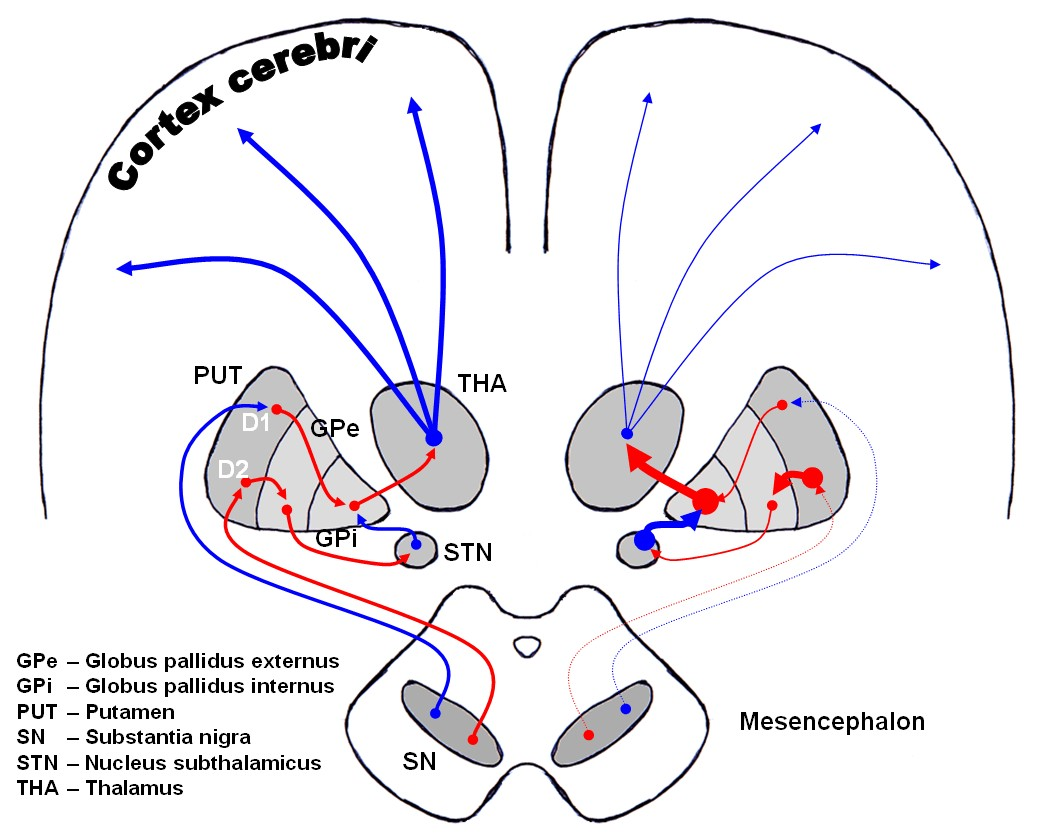
\includegraphics[width=0.5\linewidth]{FileAusiliari/Immagini/degenerative/dopamine-in-parkinsons-disease-illustration}
	\caption[Vie dopaminergiche]{L'immagine mostra le vie dopaminergiche del cervello umano in condizioni normali (a sinistra) e nella malattia di Parkinson (a destra). Le frecce rosse indicano la soppressione del bersaglio, quelle blu la stimolazione della struttura bersaglio. Caso per gentile concessione di Wikipedia, Radiopaedia.org, rID: 36286}
	\label{fig:dopamine-in-parkinsons-disease-illustration}
\end{figure*}

\subsection{Epidemiologia}
Il MP costituisce una delle principali cause di disabilità e mortalità nell'ambito delle patologie neurologiche, con una prevalenza particolarmente elevata negli Stati Uniti e in Canada (160-180 casi/100.000 abitanti). L'incidenza annuale in Nord America oscilla tra 108 e 212 casi ogni 100.000 individui di età $\geq$65 anni, con una prevalenza dello 0,3\% nella popolazione adulta $\geq$40 anni e dell'1,6\% nei soggetti ultrasessantacinquenni.
L'esordio della patologia mostra una significativa correlazione con l'età, manifestandosi tipicamente dalla quinta decade di vita, con un'età media alla diagnosi di 70,5 anni e una finestra di esordio prevalente tra i 45 e i 70 anni. Una variante giovanile può presentarsi tra i 20 e i 40 anni, sebbene l'esordio prima dei 30 anni risulti infrequente. La distribuzione per sesso evidenzia una predominanza maschile, particolarmente accentuata nella fascia d'età 50-60 anni.
L'eziologia del MP comprende fattori di rischio genetici, con particolare rilevanza nelle forme ad esordio precoce, e ambientali, tra cui l'esposizione a pesticidi e inquinanti atmosferici. Sono stati identificati fattori protettivi, inclusi il consumo di caffè, l'attività fisica e il fumo di sigaretta. La patologia si presenta prevalentemente in forma sporadica (85-90\% dei casi), mentre una minoranza dei casi (10-15\%) presenta familiarità positiva.

\subsubsection{Fattori di rischio}
L'eziopatogenesi del Morbo di Parkinson (MP) presenta una complessa interazione di fattori di rischio genetici, ambientali e non modificabili. L'anamnesi familiare positiva per MP in consanguinei di primo grado comporta un incremento del rischio relativo di 2-3 volte. Le forme monogeniche, rappresentanti meno del 10\% della casistica totale, manifestano pattern di ereditarietà autosomica dominante, recessiva o X-linked, caratterizzandosi per un esordio precoce rispetto alle forme sporadiche.
Le mutazioni eterozigoti del gene GBA1 costituiscono un significativo fattore di rischio genetico, unitamente ad alterazioni di altri geni codificanti per enzimi lisosomiali. Il coinvolgimento di geni quali SNCA, LRRK2, VPS35, Parkin, PINK1 e DJ-1 è stato ampiamente documentato. Particolare rilevanza assumono le mutazioni del gene Nurr1, determinante per l'identità neuronale dopaminergica, e del gene DJ-1, cruciale nella risposta allo stress ossidativo. Le alterazioni del gene PINK1, codificante per una chinasi mitocondriale, e del gene Park2, responsabile della sintesi della proteina parkina, sono associate a forme ad esordio precoce.
L'esposizione a neurotossine ambientali, inclusi mercurio, manganese, disolfuro di carbonio, solventi organici, MPTP e monossido di carbonio, può indurre degenerazione nigrostriatale e parkinsonismo. L'uso di neurolettici e l'abuso endovenoso di efedrone possono causare sindromi parkinsoniane potenzialmente irreversibili. Traumi cranici ripetuti, pesticidi, solventi e inquinamento atmosferico rappresentano ulteriori fattori di rischio ambientale documentati.
Tra i fattori non modificabili, l'età avanzata e il sesso maschile emergono come significativi predittori di rischio, con predominanza nella sesta decade di vita. Comorbidità quali depressione, ansia, stipsi, diabete mellito tipo 2, obesità e alterazioni del metabolismo del ferro sono state correlate a un incrementato rischio di MP.
Il consumo di tabacco e caffè, unitamente all'attività fisica regolare, ha mostrato effetti protettivi, sebbene di modesta entità. È fondamentale sottolineare che la maggioranza dei casi di MP rimane idiopatica, suggerendo un'eziologia multifattoriale.

\subsection{Presentazione  clinica}
La sintomatologia del Morbo di Parkinson manifesta un quadro clinico caratterizzato da manifestazioni motorie cardinali e sintomatologia non motoria associata. Il complesso sintomatologico motorio comprende tremore a riposo spesso asimmetrico con frequenza di 4-6 Hz, tipicamente descritto come "pill-rolling", bradicinesia manifestantesi con rallentamento motorio, ipomimia e ridotta oscillazione pendolare degli arti superiori durante la deambulazione, rigidità muscolare ("lead-pipe" o fenomeno della ruota dentata), e instabilità posturale documentabile attraverso il test della retropulsione. La deambulazione risulta caratterizzata da una progressione a piccoli passi con tendenza allo strascicamento e ridotta oscillazione degli arti superiori.
La sintomatologia accessoria include disartria con eloquio esplosivo secondario a incoordinazione linguo-diaframmatica, movimenti involontari della lingua con conseguente difficoltà protrusiva, e incremento della frequenza di ammiccamento palpebrale, quest'ultimo in contrasto con quanto osservato nella corea di Huntington. La disfunzione autonomica, i disturbi olfattivi, la sintomatologia algica, le alterazioni sensitive e i disturbi timici costituiscono il corredo sintomatologico non motorio. Il deterioramento cognitivo, con particolare coinvolgimento delle funzioni attentive, può manifestarsi e progredire nel decorso della patologia.
La progressione temporale della malattia evidenzia un esordio tipicamente unilaterale con successiva bilateralizzazione, manifestandosi prevalentemente nella sesta decade di vita. La responsività alla terapia dopaminergica, in particolare alla levodopa, rappresenta un elemento caratteristico, sebbene il tremore possa risultare farmacoresistente, in contrasto con la significativa risposta della bradicinesia e della rigidità. La variabilità fenotipica interindividuale costituisce un elemento distintivo della patologia.

\subsection{Approccio diagnostico}
L'iter diagnostico della malattia di Parkinson si fonda primariamente sulla valutazione clinica, data l'assenza di biomarcatori patognomonici. La diagnosi richiede la documentazione di bradicinesia associata ad almeno un sintomo cardine tra tremore a riposo o rigidità, valutati mediante la scala MDS-UPDRS standardizzata.
L'approccio diagnostico contempla un'accurata anamnesi ed esame obiettivo neurologico, focalizzati sull'identificazione dei sintomi cardinali: bradicinesia, tremore a riposo (4-6 Hz) tipicamente asimmetrico, rigidità e instabilità posturale. La responsività alla terapia dopaminergica, particolarmente evidente per bradicinesia e rigidità, costituisce un elemento diagnostico supportivo significativo, mentre una mancata risposta a dosaggi adeguati di levodopa suggerisce diagnosi alternative.
L'esclusione di parkinsonismi secondari richiede particolare attenzione all'insorgenza temporale dei sintomi e alla distribuzione topografica del coinvolgimento motorio. La diagnostica per immagini, sebbene non necessaria nelle presentazioni cliniche tipiche con adeguata risposta alla levodopa, può includere RM cerebrale, particolarmente utile mediante sequenze SWI per la valutazione del "swallow tail sign" nigrostriatale. La SPECT con 123I-FP-CIT (DaTscan) documenta la disfunzione dopaminergica presinaptica, mentre la PET con FDG consente la differenziazione metabolica tra PD e sindromi parkinsoniane atipiche.
L'analisi genetica, indicata in casi selezionati (esordio precoce, familiarità positiva, specifiche etnie), e la valutazione autonomica mediante scintigrafia miocardica con MIBG, che evidenzia la denervazione simpatica caratteristica, completano l'iter diagnostico. L'ecografia transcranica può evidenziare l'iperecogenicità della sostanza nera, supportando la diagnosi differenziale.
I criteri MDS stratificano la diagnosi in PD clinicamente stabilita e probabile, bilanciando specificità e sensibilità diagnostica nella pratica clinica.

\begin{Oss}
	La scala MDS-UPDRS (Movement Disorder Society-Unified Parkinson's Disease Rating Scale) è uno strumento di valutazione clinica ampiamente utilizzato per quantificare la gravità dei sintomi motori e non motori della malattia di Parkinson. Questa scala è stata sviluppata per migliorare la consistenza nella valutazione dei sintomi e per integrare meglio gli aspetti non motori della PD.
	Struttura: La scala MDS-UPDRS è composta da quattro sezioni:
	\begin{description}
		\item[Sezione I]{Esperienze non motorie della vita quotidiana. Questa sezione valuta aspetti come le capacità cognitive, i disturbi comportamentali e dell'umore}
		\item [Sezione II]{Esperienze motorie della vita quotidiana. Questa sezione valuta l'impatto dei sintomi motori sulle attività quotidiane}
		\item [Sezione III]{Esame motorio. Questa sezione valuta i segni motori della PD attraverso un esame clinico, come il tremore, la rigidità e la bradicinesia}
		\item[Sezione IV]{Complicanze della terapia. Questa sezione valuta le complicanze associate al trattamento farmacologico}
	\end{description}
	Il punteggio totale per le sezioni I-IV varia da 0 (nessuna disabilità) a 199 (disabilità totale). La sezione III, che valuta i sintomi motori, ha un punteggio che varia da 0 a 132.
	Oltre alla scala MDS-UPDRS, esistono altre scale di valutazione utilizzate nella PD, come la scala di Hoehn e Yahr e la scala di Schwab e England. La scala di Hoehn e Yahr valuta la gravità della malattia da 0 (nessuna malattia) a 5 (paziente costretto su sedia a rotelle o allettato senza assistenza).
\end{Oss}

\subsection{Anatomia patologica}
Dal punto di vista anatomopatologico il morbo di Parkinson si manifesta attraverso inclusioni proteiche intraneuronali denominate corpi di Lewy, costituiti primariamente da aggregati patologici di alfa-sinucleina, una proteina sinaptica fisiologicamente presente nel sistema nervoso centrale. L'accumulo di queste inclusioni, sebbene non patognomonico del morbo di Parkinson essendo documentabile anche nella demenza a corpi di Lewy, rappresenta una caratteristica istopatologica fondamentale quando localizzato nella substantia nigra, in associazione alla perdita neuronale dopaminergica. L'assenza di corpi di Lewy nelle forme post-encefalitiche, caratterizzate invece da grovigli neurofibrillari, e in alcune forme geneticamente determinate, sottolinea l'eterogeneità patogenetica della malattia.
La progressione spazio-temporale della patologia, codificata nello staging di Braak, delinea sei stadi evolutivi caratterizzati da una diffusione ascendente delle alterazioni neuropatologiche. Gli stadi iniziali (1-2) coinvolgono il nucleo motore dorsale dei nervi glossofaringeo e vago e il nucleo olfattivo anteriore, precedendo frequentemente la sintomatologia motoria. Gli stadi intermedi (3-4) documentano il coinvolgimento della substantia nigra pars compacta, del prosencefalo basale e della mesocorteccia temporale, correlando con l'esordio clinico della malattia. Gli stadi terminali (5-6) evidenziano una progressione neocorticale diffusa.
La patogenesi molecolare implica alterazioni del metabolismo dell'alfa-sinucleina, potenzialmente accelerate da disfunzioni delle proteine heat shock o dall'azione della dopamina. Il coinvolgimento della proteina parkin nella degradazione proteasomica evidenzia meccanismi neurodegenerativi potenzialmente indipendenti dalla formazione dei corpi di Lewy.
L'alfa-sinucleina, proteina fisiologicamente localizzata nelle terminazioni presinaptiche neuronali, manifesta nella patogenesi del morbo di Parkinson un processo patologico caratterizzato da misfolding proteico e successiva aggregazione in oligomeri, protofibrille e fibrille, culminante nella formazione dei corpi di Lewy intraneuronali. Questi aggregati proteici, considerati hallmark istopatologico della malattia, evidenziano particolare neurotossicità nella forma protofibrillare, determinando disfunzione e successiva degenerazione neuronale dopaminergica nigrostriatale.
L'identificazione di mutazioni nel gene SNCA, codificante per l'alfa-sinucleina, nelle forme familiari di malattia, unitamente alla documentazione di fenotipi clinici particolarmente aggressivi in presenza di duplicazione o triplicazione genica, ha fornito evidenze significative del ruolo causale di questa proteina nella patogenesi della malattia. La documentata capacità di trasmissione transcellulare dell'alfa-sinucleina patologica costituisce il substrato molecolare della progressione anatomopatologica descritta nello staging di Braak.
La disfunzione sinaptica correlata all'accumulo di alfa-sinucleina rappresenta un meccanismo patogenetico critico, modulato da fattori quali stress ossidativo, alterazioni del sistema ubiquitina-proteasoma e interazione con il metabolismo dopaminergico. Mutazioni nei geni parkin, PINK1 e DJ-1 influenzano il metabolismo dell'alfa-sinucleina attraverso alterazioni dei sistemi di degradazione proteica.
L'alfa-sinucleina costituisce attualmente un promettente target terapeutico, con particolare interesse per lo sviluppo di anticorpi monoclonali specifici e inibitori dell'aggregazione proteica, finalizzati al rallentamento della progressione patologica.

\subsection{Imaging}

\subsubsection{TC}
La TC manifesta un'utilità clinica circoscritta nella valutazione diagnostica primaria del MP, assumendo rilevanza nell'esclusione di patologie strutturali mimiche quali lesioni espansive, idrocefalo o alterazioni vascolari, particolarmente in presenza di presentazioni cliniche atipiche o "red flags" suggestive di diagnosi alternative.
Nel contesto della gestione terapeutica, la TC assume particolare rilevanza nella valutazione post-chirurgica della stimolazione cerebrale profonda (DBS), consentendo la verifica del corretto posizionamento degli elettrodi nel nucleo subtalamico (STN), tipicamente localizzati a 9mm dalla linea mediana, e l'identificazione di eventuali complicanze post-procedurali quali eventi emorragici, ischemici o fenomeni infiammatori transitori, questi ultimi caratterizzati da aree ipodense perilettrodiche a risoluzione graduale. L'utilità della metodica nel follow-up routinario post-DBS risulta secondaria.
La sensibilità subottimale della TC nella diagnosi differenziale tra PD e sindromi parkinsoniane atipiche, incluse atrofia multisistemica e paralisi sopranucleare progressiva, nonché nella distinzione dal tremore essenziale, ne limita significativamente l'applicazione clinica in questo contesto diagnostico.

\subsubsection{RM}
La RM è frequentemente normale nelle sequenze convenzionali (T1, T2, FLAIR) nelle fasi iniziali di malattia. L'implementazione di sequenze susceptibility-weighted imaging (SWI) o T2*-weighted ad alta risoluzione consente la visualizzazione del nigrosoma-1, struttura caratterizzata dal patognomonico "swallow tail sign", la cui perdita correla con la degenerazione dopaminergica nigrostriatale. L'accumulo patologico di ferro nella substantia nigra, quantificabile mediante sequenze SWI/T2* e incrementato del 50\% rispetto ai controlli, costituisce un ulteriore marker diagnostico, complementato dall'imaging della neuromelanina mediante sequenze T1 con impulsi di trasferimento di magnetizzazione (MTC).

\begin{figure*}[h]
	\centering
	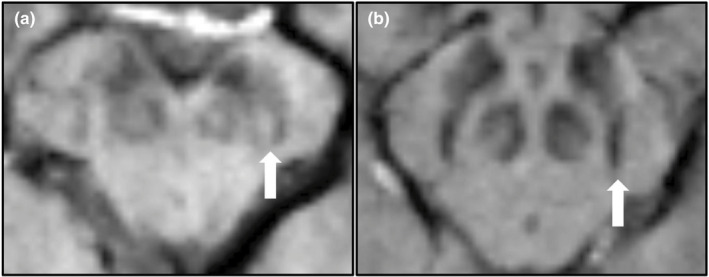
\includegraphics[width=0.8\linewidth]{FileAusiliari/Immagini/degenerative/BRB3-11-e02202-g002}
	\caption{Esempi di segno della coda di rondine (STS) in un individuo malato (a) e di STS assente in un individuo sano (b). Sono mostrate sezioni assiali del mesencefalo mappate tramite imaging pesato con suscettibilità (SWI). Le frecce bianche indicano la diversa configurazione del Nigrosoma-1 (N1). Da Brain Behav. 2021 May 24;11(7):e02202. doi: 10.1002/brb3.2202}
	\label{fig:brb3-11-e02202-g002}
\end{figure*}


La diagnosi differenziale delle sindromi parkinsoniane atipiche beneficia significativamente dell'imaging RM. L'atrofia multisistemica (MSA) evidenzia caratteristica atrofia putaminale, pontica e cerebellare, con ipointensità putaminale T2/SWI e "hot cross bun sign" pontino. La paralisi sopranucleare progressiva (PSP) manifesta atrofia mesencefalica con alterazione del rapporto mesencefalo-ponte, mentre la degenerazione corticobasale (CBD) presenta atrofia frontoparietale asimmetrica con iperintensità della sostanza bianca subcorticale.
Metodiche avanzate quali Diffusion Tensor Imaging (DTI) e risonanza magnetica funzionale (fMRI) consentono la caratterizzazione delle alterazioni microstrutturali della sostanza bianca e delle modificazioni funzionali cerebrali, sebbene la sensibilità nell'identificazione della progressione patologica e nella valutazione della risposta terapeutica necessiti ulteriore validazione. Le limitazioni metodologiche includono variabilità interindividuale e sovrapposizione dei reperti radiologici nelle diverse sindromi parkinsoniane.

\subsection{Trattamento e prognosi}

\subsection{Checklist di refertazione}

\begin{itemize}[label=$\square$] % Riquadro vuoto come simbolo
	\item Escludi altre cause di parkinsonismo (es ictus)
	\item Controlla il segnale dei nigrosomi
	\item Controlla il trofismo delle strutture sottotentoriali
\end{itemize}

\subsection{Bibliografia}
\small{
	
	
}

\note{Nota a margine}
\expl{Nota a margine colorata}
\input{Capitoli/degenerative/approccio.tex}
\input{Capitoli/degenerative/degenerative.tex}
\section{Morbo di Parkinson}

\subsection{Definizione}

\subsection{Eziologia}

\begin{figure*}[h]
	\centering
	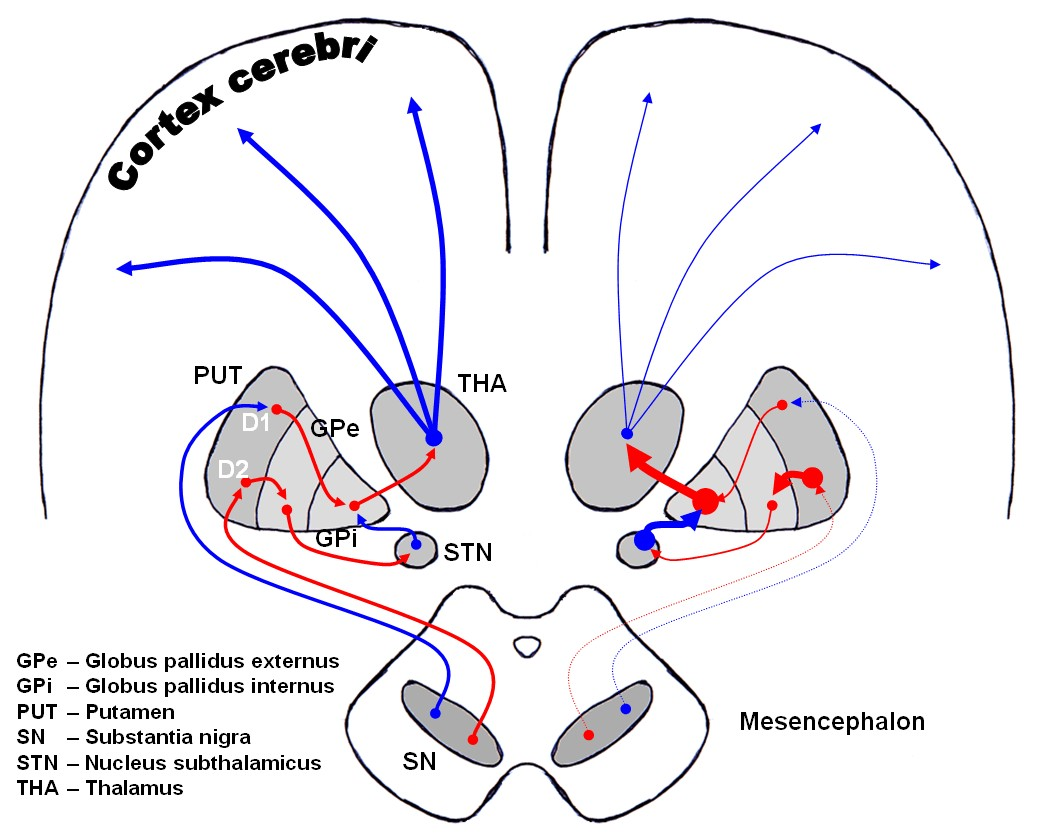
\includegraphics[width=0.5\linewidth]{FileAusiliari/Immagini/degenerative/dopamine-in-parkinsons-disease-illustration}
	\caption[Vie dopaminergiche]{L'immagine mostra le vie dopaminergiche del cervello umano in condizioni normali (a sinistra) e nella malattia di Parkinson (a destra). Le frecce rosse indicano la soppressione del bersaglio, quelle blu la stimolazione della struttura bersaglio. Caso per gentile concessione di Wikipedia, Radiopaedia.org, rID: 36286}
	\label{fig:dopamine-in-parkinsons-disease-illustration}
\end{figure*}

\subsection{Epidemiologia}
Il MP costituisce una delle principali cause di disabilità e mortalità nell'ambito delle patologie neurologiche, con una prevalenza particolarmente elevata negli Stati Uniti e in Canada (160-180 casi/100.000 abitanti). L'incidenza annuale in Nord America oscilla tra 108 e 212 casi ogni 100.000 individui di età $\geq$65 anni, con una prevalenza dello 0,3\% nella popolazione adulta $\geq$40 anni e dell'1,6\% nei soggetti ultrasessantacinquenni.
L'esordio della patologia mostra una significativa correlazione con l'età, manifestandosi tipicamente dalla quinta decade di vita, con un'età media alla diagnosi di 70,5 anni e una finestra di esordio prevalente tra i 45 e i 70 anni. Una variante giovanile può presentarsi tra i 20 e i 40 anni, sebbene l'esordio prima dei 30 anni risulti infrequente. La distribuzione per sesso evidenzia una predominanza maschile, particolarmente accentuata nella fascia d'età 50-60 anni.
L'eziologia del MP comprende fattori di rischio genetici, con particolare rilevanza nelle forme ad esordio precoce, e ambientali, tra cui l'esposizione a pesticidi e inquinanti atmosferici. Sono stati identificati fattori protettivi, inclusi il consumo di caffè, l'attività fisica e il fumo di sigaretta. La patologia si presenta prevalentemente in forma sporadica (85-90\% dei casi), mentre una minoranza dei casi (10-15\%) presenta familiarità positiva.

\subsubsection{Fattori di rischio}
L'eziopatogenesi del Morbo di Parkinson (MP) presenta una complessa interazione di fattori di rischio genetici, ambientali e non modificabili. L'anamnesi familiare positiva per MP in consanguinei di primo grado comporta un incremento del rischio relativo di 2-3 volte. Le forme monogeniche, rappresentanti meno del 10\% della casistica totale, manifestano pattern di ereditarietà autosomica dominante, recessiva o X-linked, caratterizzandosi per un esordio precoce rispetto alle forme sporadiche.
Le mutazioni eterozigoti del gene GBA1 costituiscono un significativo fattore di rischio genetico, unitamente ad alterazioni di altri geni codificanti per enzimi lisosomiali. Il coinvolgimento di geni quali SNCA, LRRK2, VPS35, Parkin, PINK1 e DJ-1 è stato ampiamente documentato. Particolare rilevanza assumono le mutazioni del gene Nurr1, determinante per l'identità neuronale dopaminergica, e del gene DJ-1, cruciale nella risposta allo stress ossidativo. Le alterazioni del gene PINK1, codificante per una chinasi mitocondriale, e del gene Park2, responsabile della sintesi della proteina parkina, sono associate a forme ad esordio precoce.
L'esposizione a neurotossine ambientali, inclusi mercurio, manganese, disolfuro di carbonio, solventi organici, MPTP e monossido di carbonio, può indurre degenerazione nigrostriatale e parkinsonismo. L'uso di neurolettici e l'abuso endovenoso di efedrone possono causare sindromi parkinsoniane potenzialmente irreversibili. Traumi cranici ripetuti, pesticidi, solventi e inquinamento atmosferico rappresentano ulteriori fattori di rischio ambientale documentati.
Tra i fattori non modificabili, l'età avanzata e il sesso maschile emergono come significativi predittori di rischio, con predominanza nella sesta decade di vita. Comorbidità quali depressione, ansia, stipsi, diabete mellito tipo 2, obesità e alterazioni del metabolismo del ferro sono state correlate a un incrementato rischio di MP.
Il consumo di tabacco e caffè, unitamente all'attività fisica regolare, ha mostrato effetti protettivi, sebbene di modesta entità. È fondamentale sottolineare che la maggioranza dei casi di MP rimane idiopatica, suggerendo un'eziologia multifattoriale.

\subsection{Presentazione  clinica}
La sintomatologia del Morbo di Parkinson manifesta un quadro clinico caratterizzato da manifestazioni motorie cardinali e sintomatologia non motoria associata. Il complesso sintomatologico motorio comprende tremore a riposo spesso asimmetrico con frequenza di 4-6 Hz, tipicamente descritto come "pill-rolling", bradicinesia manifestantesi con rallentamento motorio, ipomimia e ridotta oscillazione pendolare degli arti superiori durante la deambulazione, rigidità muscolare ("lead-pipe" o fenomeno della ruota dentata), e instabilità posturale documentabile attraverso il test della retropulsione. La deambulazione risulta caratterizzata da una progressione a piccoli passi con tendenza allo strascicamento e ridotta oscillazione degli arti superiori.
La sintomatologia accessoria include disartria con eloquio esplosivo secondario a incoordinazione linguo-diaframmatica, movimenti involontari della lingua con conseguente difficoltà protrusiva, e incremento della frequenza di ammiccamento palpebrale, quest'ultimo in contrasto con quanto osservato nella corea di Huntington. La disfunzione autonomica, i disturbi olfattivi, la sintomatologia algica, le alterazioni sensitive e i disturbi timici costituiscono il corredo sintomatologico non motorio. Il deterioramento cognitivo, con particolare coinvolgimento delle funzioni attentive, può manifestarsi e progredire nel decorso della patologia.
La progressione temporale della malattia evidenzia un esordio tipicamente unilaterale con successiva bilateralizzazione, manifestandosi prevalentemente nella sesta decade di vita. La responsività alla terapia dopaminergica, in particolare alla levodopa, rappresenta un elemento caratteristico, sebbene il tremore possa risultare farmacoresistente, in contrasto con la significativa risposta della bradicinesia e della rigidità. La variabilità fenotipica interindividuale costituisce un elemento distintivo della patologia.

\subsection{Approccio diagnostico}
L'iter diagnostico della malattia di Parkinson si fonda primariamente sulla valutazione clinica, data l'assenza di biomarcatori patognomonici. La diagnosi richiede la documentazione di bradicinesia associata ad almeno un sintomo cardine tra tremore a riposo o rigidità, valutati mediante la scala MDS-UPDRS standardizzata.
L'approccio diagnostico contempla un'accurata anamnesi ed esame obiettivo neurologico, focalizzati sull'identificazione dei sintomi cardinali: bradicinesia, tremore a riposo (4-6 Hz) tipicamente asimmetrico, rigidità e instabilità posturale. La responsività alla terapia dopaminergica, particolarmente evidente per bradicinesia e rigidità, costituisce un elemento diagnostico supportivo significativo, mentre una mancata risposta a dosaggi adeguati di levodopa suggerisce diagnosi alternative.
L'esclusione di parkinsonismi secondari richiede particolare attenzione all'insorgenza temporale dei sintomi e alla distribuzione topografica del coinvolgimento motorio. La diagnostica per immagini, sebbene non necessaria nelle presentazioni cliniche tipiche con adeguata risposta alla levodopa, può includere RM cerebrale, particolarmente utile mediante sequenze SWI per la valutazione del "swallow tail sign" nigrostriatale. La SPECT con 123I-FP-CIT (DaTscan) documenta la disfunzione dopaminergica presinaptica, mentre la PET con FDG consente la differenziazione metabolica tra PD e sindromi parkinsoniane atipiche.
L'analisi genetica, indicata in casi selezionati (esordio precoce, familiarità positiva, specifiche etnie), e la valutazione autonomica mediante scintigrafia miocardica con MIBG, che evidenzia la denervazione simpatica caratteristica, completano l'iter diagnostico. L'ecografia transcranica può evidenziare l'iperecogenicità della sostanza nera, supportando la diagnosi differenziale.
I criteri MDS stratificano la diagnosi in PD clinicamente stabilita e probabile, bilanciando specificità e sensibilità diagnostica nella pratica clinica.

\begin{Oss}
	La scala MDS-UPDRS (Movement Disorder Society-Unified Parkinson's Disease Rating Scale) è uno strumento di valutazione clinica ampiamente utilizzato per quantificare la gravità dei sintomi motori e non motori della malattia di Parkinson. Questa scala è stata sviluppata per migliorare la consistenza nella valutazione dei sintomi e per integrare meglio gli aspetti non motori della PD.
	Struttura: La scala MDS-UPDRS è composta da quattro sezioni:
	\begin{description}
		\item[Sezione I]{Esperienze non motorie della vita quotidiana. Questa sezione valuta aspetti come le capacità cognitive, i disturbi comportamentali e dell'umore}
		\item [Sezione II]{Esperienze motorie della vita quotidiana. Questa sezione valuta l'impatto dei sintomi motori sulle attività quotidiane}
		\item [Sezione III]{Esame motorio. Questa sezione valuta i segni motori della PD attraverso un esame clinico, come il tremore, la rigidità e la bradicinesia}
		\item[Sezione IV]{Complicanze della terapia. Questa sezione valuta le complicanze associate al trattamento farmacologico}
	\end{description}
	Il punteggio totale per le sezioni I-IV varia da 0 (nessuna disabilità) a 199 (disabilità totale). La sezione III, che valuta i sintomi motori, ha un punteggio che varia da 0 a 132.
	Oltre alla scala MDS-UPDRS, esistono altre scale di valutazione utilizzate nella PD, come la scala di Hoehn e Yahr e la scala di Schwab e England. La scala di Hoehn e Yahr valuta la gravità della malattia da 0 (nessuna malattia) a 5 (paziente costretto su sedia a rotelle o allettato senza assistenza).
\end{Oss}

\subsection{Anatomia patologica}
Dal punto di vista anatomopatologico il morbo di Parkinson si manifesta attraverso inclusioni proteiche intraneuronali denominate corpi di Lewy, costituiti primariamente da aggregati patologici di alfa-sinucleina, una proteina sinaptica fisiologicamente presente nel sistema nervoso centrale. L'accumulo di queste inclusioni, sebbene non patognomonico del morbo di Parkinson essendo documentabile anche nella demenza a corpi di Lewy, rappresenta una caratteristica istopatologica fondamentale quando localizzato nella substantia nigra, in associazione alla perdita neuronale dopaminergica. L'assenza di corpi di Lewy nelle forme post-encefalitiche, caratterizzate invece da grovigli neurofibrillari, e in alcune forme geneticamente determinate, sottolinea l'eterogeneità patogenetica della malattia.
La progressione spazio-temporale della patologia, codificata nello staging di Braak, delinea sei stadi evolutivi caratterizzati da una diffusione ascendente delle alterazioni neuropatologiche. Gli stadi iniziali (1-2) coinvolgono il nucleo motore dorsale dei nervi glossofaringeo e vago e il nucleo olfattivo anteriore, precedendo frequentemente la sintomatologia motoria. Gli stadi intermedi (3-4) documentano il coinvolgimento della substantia nigra pars compacta, del prosencefalo basale e della mesocorteccia temporale, correlando con l'esordio clinico della malattia. Gli stadi terminali (5-6) evidenziano una progressione neocorticale diffusa.
La patogenesi molecolare implica alterazioni del metabolismo dell'alfa-sinucleina, potenzialmente accelerate da disfunzioni delle proteine heat shock o dall'azione della dopamina. Il coinvolgimento della proteina parkin nella degradazione proteasomica evidenzia meccanismi neurodegenerativi potenzialmente indipendenti dalla formazione dei corpi di Lewy.
L'alfa-sinucleina, proteina fisiologicamente localizzata nelle terminazioni presinaptiche neuronali, manifesta nella patogenesi del morbo di Parkinson un processo patologico caratterizzato da misfolding proteico e successiva aggregazione in oligomeri, protofibrille e fibrille, culminante nella formazione dei corpi di Lewy intraneuronali. Questi aggregati proteici, considerati hallmark istopatologico della malattia, evidenziano particolare neurotossicità nella forma protofibrillare, determinando disfunzione e successiva degenerazione neuronale dopaminergica nigrostriatale.
L'identificazione di mutazioni nel gene SNCA, codificante per l'alfa-sinucleina, nelle forme familiari di malattia, unitamente alla documentazione di fenotipi clinici particolarmente aggressivi in presenza di duplicazione o triplicazione genica, ha fornito evidenze significative del ruolo causale di questa proteina nella patogenesi della malattia. La documentata capacità di trasmissione transcellulare dell'alfa-sinucleina patologica costituisce il substrato molecolare della progressione anatomopatologica descritta nello staging di Braak.
La disfunzione sinaptica correlata all'accumulo di alfa-sinucleina rappresenta un meccanismo patogenetico critico, modulato da fattori quali stress ossidativo, alterazioni del sistema ubiquitina-proteasoma e interazione con il metabolismo dopaminergico. Mutazioni nei geni parkin, PINK1 e DJ-1 influenzano il metabolismo dell'alfa-sinucleina attraverso alterazioni dei sistemi di degradazione proteica.
L'alfa-sinucleina costituisce attualmente un promettente target terapeutico, con particolare interesse per lo sviluppo di anticorpi monoclonali specifici e inibitori dell'aggregazione proteica, finalizzati al rallentamento della progressione patologica.

\subsection{Imaging}

\subsubsection{TC}
La TC manifesta un'utilità clinica circoscritta nella valutazione diagnostica primaria del MP, assumendo rilevanza nell'esclusione di patologie strutturali mimiche quali lesioni espansive, idrocefalo o alterazioni vascolari, particolarmente in presenza di presentazioni cliniche atipiche o "red flags" suggestive di diagnosi alternative.
Nel contesto della gestione terapeutica, la TC assume particolare rilevanza nella valutazione post-chirurgica della stimolazione cerebrale profonda (DBS), consentendo la verifica del corretto posizionamento degli elettrodi nel nucleo subtalamico (STN), tipicamente localizzati a 9mm dalla linea mediana, e l'identificazione di eventuali complicanze post-procedurali quali eventi emorragici, ischemici o fenomeni infiammatori transitori, questi ultimi caratterizzati da aree ipodense perilettrodiche a risoluzione graduale. L'utilità della metodica nel follow-up routinario post-DBS risulta secondaria.
La sensibilità subottimale della TC nella diagnosi differenziale tra PD e sindromi parkinsoniane atipiche, incluse atrofia multisistemica e paralisi sopranucleare progressiva, nonché nella distinzione dal tremore essenziale, ne limita significativamente l'applicazione clinica in questo contesto diagnostico.

\subsubsection{RM}
La RM è frequentemente normale nelle sequenze convenzionali (T1, T2, FLAIR) nelle fasi iniziali di malattia. L'implementazione di sequenze susceptibility-weighted imaging (SWI) o T2*-weighted ad alta risoluzione consente la visualizzazione del nigrosoma-1, struttura caratterizzata dal patognomonico "swallow tail sign", la cui perdita correla con la degenerazione dopaminergica nigrostriatale. L'accumulo patologico di ferro nella substantia nigra, quantificabile mediante sequenze SWI/T2* e incrementato del 50\% rispetto ai controlli, costituisce un ulteriore marker diagnostico, complementato dall'imaging della neuromelanina mediante sequenze T1 con impulsi di trasferimento di magnetizzazione (MTC).

\begin{figure*}[h]
	\centering
	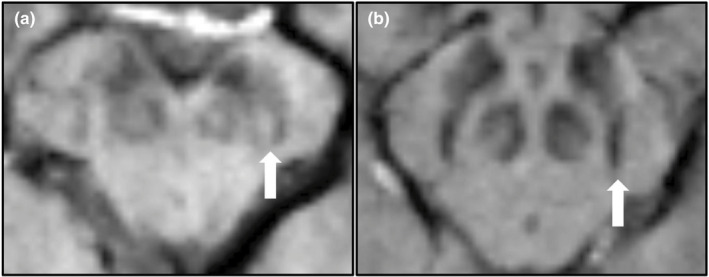
\includegraphics[width=0.8\linewidth]{FileAusiliari/Immagini/degenerative/BRB3-11-e02202-g002}
	\caption{Esempi di segno della coda di rondine (STS) in un individuo malato (a) e di STS assente in un individuo sano (b). Sono mostrate sezioni assiali del mesencefalo mappate tramite imaging pesato con suscettibilità (SWI). Le frecce bianche indicano la diversa configurazione del Nigrosoma-1 (N1). Da Brain Behav. 2021 May 24;11(7):e02202. doi: 10.1002/brb3.2202}
	\label{fig:brb3-11-e02202-g002}
\end{figure*}


La diagnosi differenziale delle sindromi parkinsoniane atipiche beneficia significativamente dell'imaging RM. L'atrofia multisistemica (MSA) evidenzia caratteristica atrofia putaminale, pontica e cerebellare, con ipointensità putaminale T2/SWI e "hot cross bun sign" pontino. La paralisi sopranucleare progressiva (PSP) manifesta atrofia mesencefalica con alterazione del rapporto mesencefalo-ponte, mentre la degenerazione corticobasale (CBD) presenta atrofia frontoparietale asimmetrica con iperintensità della sostanza bianca subcorticale.
Metodiche avanzate quali Diffusion Tensor Imaging (DTI) e risonanza magnetica funzionale (fMRI) consentono la caratterizzazione delle alterazioni microstrutturali della sostanza bianca e delle modificazioni funzionali cerebrali, sebbene la sensibilità nell'identificazione della progressione patologica e nella valutazione della risposta terapeutica necessiti ulteriore validazione. Le limitazioni metodologiche includono variabilità interindividuale e sovrapposizione dei reperti radiologici nelle diverse sindromi parkinsoniane.

\subsection{Trattamento e prognosi}

\subsection{Checklist di refertazione}

\begin{itemize}[label=$\square$] % Riquadro vuoto come simbolo
	\item Escludi altre cause di parkinsonismo (es ictus)
	\item Controlla il segnale dei nigrosomi
	\item Controlla il trofismo delle strutture sottotentoriali
\end{itemize}

\subsection{Bibliografia}
\small{
	
	
}

\note{Nota a margine}
\expl{Nota a margine colorata}
\input{Capitoli/degenerative/approccio.tex}
\input{Capitoli/degenerative/degenerative.tex}
\section{Morbo di Parkinson}

\subsection{Definizione}

\subsection{Eziologia}

\begin{figure*}[h]
	\centering
	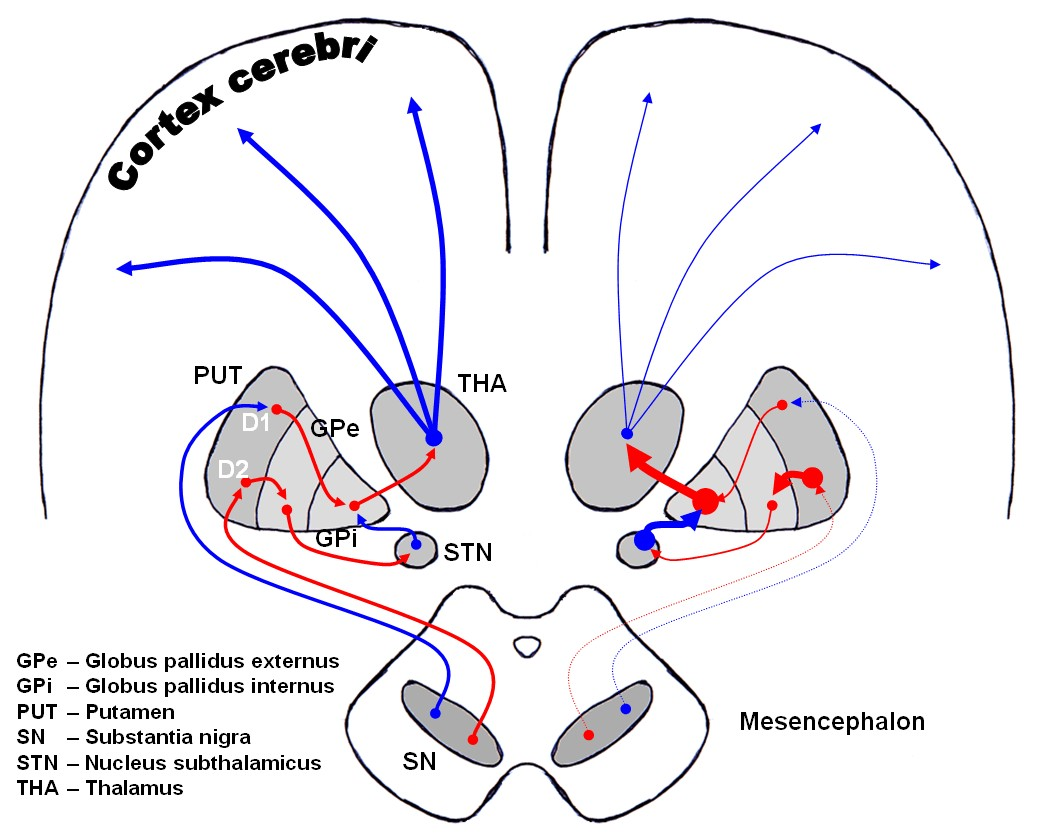
\includegraphics[width=0.5\linewidth]{FileAusiliari/Immagini/degenerative/dopamine-in-parkinsons-disease-illustration}
	\caption[Vie dopaminergiche]{L'immagine mostra le vie dopaminergiche del cervello umano in condizioni normali (a sinistra) e nella malattia di Parkinson (a destra). Le frecce rosse indicano la soppressione del bersaglio, quelle blu la stimolazione della struttura bersaglio. Caso per gentile concessione di Wikipedia, Radiopaedia.org, rID: 36286}
	\label{fig:dopamine-in-parkinsons-disease-illustration}
\end{figure*}

\subsection{Epidemiologia}
Il MP costituisce una delle principali cause di disabilità e mortalità nell'ambito delle patologie neurologiche, con una prevalenza particolarmente elevata negli Stati Uniti e in Canada (160-180 casi/100.000 abitanti). L'incidenza annuale in Nord America oscilla tra 108 e 212 casi ogni 100.000 individui di età $\geq$65 anni, con una prevalenza dello 0,3\% nella popolazione adulta $\geq$40 anni e dell'1,6\% nei soggetti ultrasessantacinquenni.
L'esordio della patologia mostra una significativa correlazione con l'età, manifestandosi tipicamente dalla quinta decade di vita, con un'età media alla diagnosi di 70,5 anni e una finestra di esordio prevalente tra i 45 e i 70 anni. Una variante giovanile può presentarsi tra i 20 e i 40 anni, sebbene l'esordio prima dei 30 anni risulti infrequente. La distribuzione per sesso evidenzia una predominanza maschile, particolarmente accentuata nella fascia d'età 50-60 anni.
L'eziologia del MP comprende fattori di rischio genetici, con particolare rilevanza nelle forme ad esordio precoce, e ambientali, tra cui l'esposizione a pesticidi e inquinanti atmosferici. Sono stati identificati fattori protettivi, inclusi il consumo di caffè, l'attività fisica e il fumo di sigaretta. La patologia si presenta prevalentemente in forma sporadica (85-90\% dei casi), mentre una minoranza dei casi (10-15\%) presenta familiarità positiva.

\subsubsection{Fattori di rischio}
L'eziopatogenesi del Morbo di Parkinson (MP) presenta una complessa interazione di fattori di rischio genetici, ambientali e non modificabili. L'anamnesi familiare positiva per MP in consanguinei di primo grado comporta un incremento del rischio relativo di 2-3 volte. Le forme monogeniche, rappresentanti meno del 10\% della casistica totale, manifestano pattern di ereditarietà autosomica dominante, recessiva o X-linked, caratterizzandosi per un esordio precoce rispetto alle forme sporadiche.
Le mutazioni eterozigoti del gene GBA1 costituiscono un significativo fattore di rischio genetico, unitamente ad alterazioni di altri geni codificanti per enzimi lisosomiali. Il coinvolgimento di geni quali SNCA, LRRK2, VPS35, Parkin, PINK1 e DJ-1 è stato ampiamente documentato. Particolare rilevanza assumono le mutazioni del gene Nurr1, determinante per l'identità neuronale dopaminergica, e del gene DJ-1, cruciale nella risposta allo stress ossidativo. Le alterazioni del gene PINK1, codificante per una chinasi mitocondriale, e del gene Park2, responsabile della sintesi della proteina parkina, sono associate a forme ad esordio precoce.
L'esposizione a neurotossine ambientali, inclusi mercurio, manganese, disolfuro di carbonio, solventi organici, MPTP e monossido di carbonio, può indurre degenerazione nigrostriatale e parkinsonismo. L'uso di neurolettici e l'abuso endovenoso di efedrone possono causare sindromi parkinsoniane potenzialmente irreversibili. Traumi cranici ripetuti, pesticidi, solventi e inquinamento atmosferico rappresentano ulteriori fattori di rischio ambientale documentati.
Tra i fattori non modificabili, l'età avanzata e il sesso maschile emergono come significativi predittori di rischio, con predominanza nella sesta decade di vita. Comorbidità quali depressione, ansia, stipsi, diabete mellito tipo 2, obesità e alterazioni del metabolismo del ferro sono state correlate a un incrementato rischio di MP.
Il consumo di tabacco e caffè, unitamente all'attività fisica regolare, ha mostrato effetti protettivi, sebbene di modesta entità. È fondamentale sottolineare che la maggioranza dei casi di MP rimane idiopatica, suggerendo un'eziologia multifattoriale.

\subsection{Presentazione  clinica}
La sintomatologia del Morbo di Parkinson manifesta un quadro clinico caratterizzato da manifestazioni motorie cardinali e sintomatologia non motoria associata. Il complesso sintomatologico motorio comprende tremore a riposo spesso asimmetrico con frequenza di 4-6 Hz, tipicamente descritto come "pill-rolling", bradicinesia manifestantesi con rallentamento motorio, ipomimia e ridotta oscillazione pendolare degli arti superiori durante la deambulazione, rigidità muscolare ("lead-pipe" o fenomeno della ruota dentata), e instabilità posturale documentabile attraverso il test della retropulsione. La deambulazione risulta caratterizzata da una progressione a piccoli passi con tendenza allo strascicamento e ridotta oscillazione degli arti superiori.
La sintomatologia accessoria include disartria con eloquio esplosivo secondario a incoordinazione linguo-diaframmatica, movimenti involontari della lingua con conseguente difficoltà protrusiva, e incremento della frequenza di ammiccamento palpebrale, quest'ultimo in contrasto con quanto osservato nella corea di Huntington. La disfunzione autonomica, i disturbi olfattivi, la sintomatologia algica, le alterazioni sensitive e i disturbi timici costituiscono il corredo sintomatologico non motorio. Il deterioramento cognitivo, con particolare coinvolgimento delle funzioni attentive, può manifestarsi e progredire nel decorso della patologia.
La progressione temporale della malattia evidenzia un esordio tipicamente unilaterale con successiva bilateralizzazione, manifestandosi prevalentemente nella sesta decade di vita. La responsività alla terapia dopaminergica, in particolare alla levodopa, rappresenta un elemento caratteristico, sebbene il tremore possa risultare farmacoresistente, in contrasto con la significativa risposta della bradicinesia e della rigidità. La variabilità fenotipica interindividuale costituisce un elemento distintivo della patologia.

\subsection{Approccio diagnostico}
L'iter diagnostico della malattia di Parkinson si fonda primariamente sulla valutazione clinica, data l'assenza di biomarcatori patognomonici. La diagnosi richiede la documentazione di bradicinesia associata ad almeno un sintomo cardine tra tremore a riposo o rigidità, valutati mediante la scala MDS-UPDRS standardizzata.
L'approccio diagnostico contempla un'accurata anamnesi ed esame obiettivo neurologico, focalizzati sull'identificazione dei sintomi cardinali: bradicinesia, tremore a riposo (4-6 Hz) tipicamente asimmetrico, rigidità e instabilità posturale. La responsività alla terapia dopaminergica, particolarmente evidente per bradicinesia e rigidità, costituisce un elemento diagnostico supportivo significativo, mentre una mancata risposta a dosaggi adeguati di levodopa suggerisce diagnosi alternative.
L'esclusione di parkinsonismi secondari richiede particolare attenzione all'insorgenza temporale dei sintomi e alla distribuzione topografica del coinvolgimento motorio. La diagnostica per immagini, sebbene non necessaria nelle presentazioni cliniche tipiche con adeguata risposta alla levodopa, può includere RM cerebrale, particolarmente utile mediante sequenze SWI per la valutazione del "swallow tail sign" nigrostriatale. La SPECT con 123I-FP-CIT (DaTscan) documenta la disfunzione dopaminergica presinaptica, mentre la PET con FDG consente la differenziazione metabolica tra PD e sindromi parkinsoniane atipiche.
L'analisi genetica, indicata in casi selezionati (esordio precoce, familiarità positiva, specifiche etnie), e la valutazione autonomica mediante scintigrafia miocardica con MIBG, che evidenzia la denervazione simpatica caratteristica, completano l'iter diagnostico. L'ecografia transcranica può evidenziare l'iperecogenicità della sostanza nera, supportando la diagnosi differenziale.
I criteri MDS stratificano la diagnosi in PD clinicamente stabilita e probabile, bilanciando specificità e sensibilità diagnostica nella pratica clinica.

\begin{Oss}
	La scala MDS-UPDRS (Movement Disorder Society-Unified Parkinson's Disease Rating Scale) è uno strumento di valutazione clinica ampiamente utilizzato per quantificare la gravità dei sintomi motori e non motori della malattia di Parkinson. Questa scala è stata sviluppata per migliorare la consistenza nella valutazione dei sintomi e per integrare meglio gli aspetti non motori della PD.
	Struttura: La scala MDS-UPDRS è composta da quattro sezioni:
	\begin{description}
		\item[Sezione I]{Esperienze non motorie della vita quotidiana. Questa sezione valuta aspetti come le capacità cognitive, i disturbi comportamentali e dell'umore}
		\item [Sezione II]{Esperienze motorie della vita quotidiana. Questa sezione valuta l'impatto dei sintomi motori sulle attività quotidiane}
		\item [Sezione III]{Esame motorio. Questa sezione valuta i segni motori della PD attraverso un esame clinico, come il tremore, la rigidità e la bradicinesia}
		\item[Sezione IV]{Complicanze della terapia. Questa sezione valuta le complicanze associate al trattamento farmacologico}
	\end{description}
	Il punteggio totale per le sezioni I-IV varia da 0 (nessuna disabilità) a 199 (disabilità totale). La sezione III, che valuta i sintomi motori, ha un punteggio che varia da 0 a 132.
	Oltre alla scala MDS-UPDRS, esistono altre scale di valutazione utilizzate nella PD, come la scala di Hoehn e Yahr e la scala di Schwab e England. La scala di Hoehn e Yahr valuta la gravità della malattia da 0 (nessuna malattia) a 5 (paziente costretto su sedia a rotelle o allettato senza assistenza).
\end{Oss}

\subsection{Anatomia patologica}
Dal punto di vista anatomopatologico il morbo di Parkinson si manifesta attraverso inclusioni proteiche intraneuronali denominate corpi di Lewy, costituiti primariamente da aggregati patologici di alfa-sinucleina, una proteina sinaptica fisiologicamente presente nel sistema nervoso centrale. L'accumulo di queste inclusioni, sebbene non patognomonico del morbo di Parkinson essendo documentabile anche nella demenza a corpi di Lewy, rappresenta una caratteristica istopatologica fondamentale quando localizzato nella substantia nigra, in associazione alla perdita neuronale dopaminergica. L'assenza di corpi di Lewy nelle forme post-encefalitiche, caratterizzate invece da grovigli neurofibrillari, e in alcune forme geneticamente determinate, sottolinea l'eterogeneità patogenetica della malattia.
La progressione spazio-temporale della patologia, codificata nello staging di Braak, delinea sei stadi evolutivi caratterizzati da una diffusione ascendente delle alterazioni neuropatologiche. Gli stadi iniziali (1-2) coinvolgono il nucleo motore dorsale dei nervi glossofaringeo e vago e il nucleo olfattivo anteriore, precedendo frequentemente la sintomatologia motoria. Gli stadi intermedi (3-4) documentano il coinvolgimento della substantia nigra pars compacta, del prosencefalo basale e della mesocorteccia temporale, correlando con l'esordio clinico della malattia. Gli stadi terminali (5-6) evidenziano una progressione neocorticale diffusa.
La patogenesi molecolare implica alterazioni del metabolismo dell'alfa-sinucleina, potenzialmente accelerate da disfunzioni delle proteine heat shock o dall'azione della dopamina. Il coinvolgimento della proteina parkin nella degradazione proteasomica evidenzia meccanismi neurodegenerativi potenzialmente indipendenti dalla formazione dei corpi di Lewy.
L'alfa-sinucleina, proteina fisiologicamente localizzata nelle terminazioni presinaptiche neuronali, manifesta nella patogenesi del morbo di Parkinson un processo patologico caratterizzato da misfolding proteico e successiva aggregazione in oligomeri, protofibrille e fibrille, culminante nella formazione dei corpi di Lewy intraneuronali. Questi aggregati proteici, considerati hallmark istopatologico della malattia, evidenziano particolare neurotossicità nella forma protofibrillare, determinando disfunzione e successiva degenerazione neuronale dopaminergica nigrostriatale.
L'identificazione di mutazioni nel gene SNCA, codificante per l'alfa-sinucleina, nelle forme familiari di malattia, unitamente alla documentazione di fenotipi clinici particolarmente aggressivi in presenza di duplicazione o triplicazione genica, ha fornito evidenze significative del ruolo causale di questa proteina nella patogenesi della malattia. La documentata capacità di trasmissione transcellulare dell'alfa-sinucleina patologica costituisce il substrato molecolare della progressione anatomopatologica descritta nello staging di Braak.
La disfunzione sinaptica correlata all'accumulo di alfa-sinucleina rappresenta un meccanismo patogenetico critico, modulato da fattori quali stress ossidativo, alterazioni del sistema ubiquitina-proteasoma e interazione con il metabolismo dopaminergico. Mutazioni nei geni parkin, PINK1 e DJ-1 influenzano il metabolismo dell'alfa-sinucleina attraverso alterazioni dei sistemi di degradazione proteica.
L'alfa-sinucleina costituisce attualmente un promettente target terapeutico, con particolare interesse per lo sviluppo di anticorpi monoclonali specifici e inibitori dell'aggregazione proteica, finalizzati al rallentamento della progressione patologica.

\subsection{Imaging}

\subsubsection{TC}
La TC manifesta un'utilità clinica circoscritta nella valutazione diagnostica primaria del MP, assumendo rilevanza nell'esclusione di patologie strutturali mimiche quali lesioni espansive, idrocefalo o alterazioni vascolari, particolarmente in presenza di presentazioni cliniche atipiche o "red flags" suggestive di diagnosi alternative.
Nel contesto della gestione terapeutica, la TC assume particolare rilevanza nella valutazione post-chirurgica della stimolazione cerebrale profonda (DBS), consentendo la verifica del corretto posizionamento degli elettrodi nel nucleo subtalamico (STN), tipicamente localizzati a 9mm dalla linea mediana, e l'identificazione di eventuali complicanze post-procedurali quali eventi emorragici, ischemici o fenomeni infiammatori transitori, questi ultimi caratterizzati da aree ipodense perilettrodiche a risoluzione graduale. L'utilità della metodica nel follow-up routinario post-DBS risulta secondaria.
La sensibilità subottimale della TC nella diagnosi differenziale tra PD e sindromi parkinsoniane atipiche, incluse atrofia multisistemica e paralisi sopranucleare progressiva, nonché nella distinzione dal tremore essenziale, ne limita significativamente l'applicazione clinica in questo contesto diagnostico.

\subsubsection{RM}
La RM è frequentemente normale nelle sequenze convenzionali (T1, T2, FLAIR) nelle fasi iniziali di malattia. L'implementazione di sequenze susceptibility-weighted imaging (SWI) o T2*-weighted ad alta risoluzione consente la visualizzazione del nigrosoma-1, struttura caratterizzata dal patognomonico "swallow tail sign", la cui perdita correla con la degenerazione dopaminergica nigrostriatale. L'accumulo patologico di ferro nella substantia nigra, quantificabile mediante sequenze SWI/T2* e incrementato del 50\% rispetto ai controlli, costituisce un ulteriore marker diagnostico, complementato dall'imaging della neuromelanina mediante sequenze T1 con impulsi di trasferimento di magnetizzazione (MTC).

\begin{figure*}[h]
	\centering
	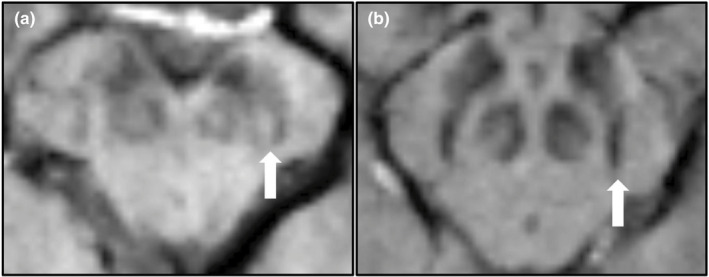
\includegraphics[width=0.8\linewidth]{FileAusiliari/Immagini/degenerative/BRB3-11-e02202-g002}
	\caption{Esempi di segno della coda di rondine (STS) in un individuo malato (a) e di STS assente in un individuo sano (b). Sono mostrate sezioni assiali del mesencefalo mappate tramite imaging pesato con suscettibilità (SWI). Le frecce bianche indicano la diversa configurazione del Nigrosoma-1 (N1). Da Brain Behav. 2021 May 24;11(7):e02202. doi: 10.1002/brb3.2202}
	\label{fig:brb3-11-e02202-g002}
\end{figure*}


La diagnosi differenziale delle sindromi parkinsoniane atipiche beneficia significativamente dell'imaging RM. L'atrofia multisistemica (MSA) evidenzia caratteristica atrofia putaminale, pontica e cerebellare, con ipointensità putaminale T2/SWI e "hot cross bun sign" pontino. La paralisi sopranucleare progressiva (PSP) manifesta atrofia mesencefalica con alterazione del rapporto mesencefalo-ponte, mentre la degenerazione corticobasale (CBD) presenta atrofia frontoparietale asimmetrica con iperintensità della sostanza bianca subcorticale.
Metodiche avanzate quali Diffusion Tensor Imaging (DTI) e risonanza magnetica funzionale (fMRI) consentono la caratterizzazione delle alterazioni microstrutturali della sostanza bianca e delle modificazioni funzionali cerebrali, sebbene la sensibilità nell'identificazione della progressione patologica e nella valutazione della risposta terapeutica necessiti ulteriore validazione. Le limitazioni metodologiche includono variabilità interindividuale e sovrapposizione dei reperti radiologici nelle diverse sindromi parkinsoniane.

\subsection{Trattamento e prognosi}

\subsection{Checklist di refertazione}

\begin{itemize}[label=$\square$] % Riquadro vuoto come simbolo
	\item Escludi altre cause di parkinsonismo (es ictus)
	\item Controlla il segnale dei nigrosomi
	\item Controlla il trofismo delle strutture sottotentoriali
\end{itemize}

\subsection{Bibliografia}
\small{
	
	
}

\note{Nota a margine}
\expl{Nota a margine colorata}
\input{Capitoli/degenerative/approccio.tex}
\input{Capitoli/degenerative/degenerative.tex}
\section{Morbo di Parkinson}

\subsection{Definizione}

\subsection{Eziologia}

\begin{figure*}[h]
	\centering
	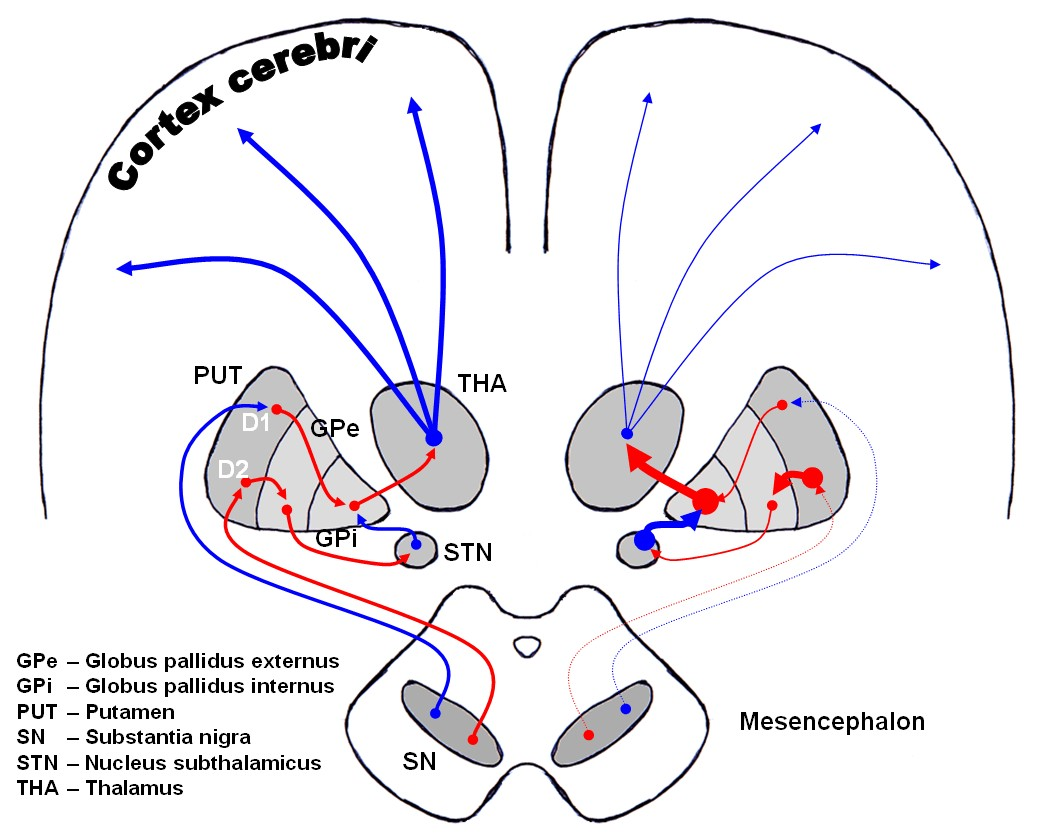
\includegraphics[width=0.5\linewidth]{FileAusiliari/Immagini/degenerative/dopamine-in-parkinsons-disease-illustration}
	\caption[Vie dopaminergiche]{L'immagine mostra le vie dopaminergiche del cervello umano in condizioni normali (a sinistra) e nella malattia di Parkinson (a destra). Le frecce rosse indicano la soppressione del bersaglio, quelle blu la stimolazione della struttura bersaglio. Caso per gentile concessione di Wikipedia, Radiopaedia.org, rID: 36286}
	\label{fig:dopamine-in-parkinsons-disease-illustration}
\end{figure*}

\subsection{Epidemiologia}
Il MP costituisce una delle principali cause di disabilità e mortalità nell'ambito delle patologie neurologiche, con una prevalenza particolarmente elevata negli Stati Uniti e in Canada (160-180 casi/100.000 abitanti). L'incidenza annuale in Nord America oscilla tra 108 e 212 casi ogni 100.000 individui di età $\geq$65 anni, con una prevalenza dello 0,3\% nella popolazione adulta $\geq$40 anni e dell'1,6\% nei soggetti ultrasessantacinquenni.
L'esordio della patologia mostra una significativa correlazione con l'età, manifestandosi tipicamente dalla quinta decade di vita, con un'età media alla diagnosi di 70,5 anni e una finestra di esordio prevalente tra i 45 e i 70 anni. Una variante giovanile può presentarsi tra i 20 e i 40 anni, sebbene l'esordio prima dei 30 anni risulti infrequente. La distribuzione per sesso evidenzia una predominanza maschile, particolarmente accentuata nella fascia d'età 50-60 anni.
L'eziologia del MP comprende fattori di rischio genetici, con particolare rilevanza nelle forme ad esordio precoce, e ambientali, tra cui l'esposizione a pesticidi e inquinanti atmosferici. Sono stati identificati fattori protettivi, inclusi il consumo di caffè, l'attività fisica e il fumo di sigaretta. La patologia si presenta prevalentemente in forma sporadica (85-90\% dei casi), mentre una minoranza dei casi (10-15\%) presenta familiarità positiva.

\subsubsection{Fattori di rischio}
L'eziopatogenesi del Morbo di Parkinson (MP) presenta una complessa interazione di fattori di rischio genetici, ambientali e non modificabili. L'anamnesi familiare positiva per MP in consanguinei di primo grado comporta un incremento del rischio relativo di 2-3 volte. Le forme monogeniche, rappresentanti meno del 10\% della casistica totale, manifestano pattern di ereditarietà autosomica dominante, recessiva o X-linked, caratterizzandosi per un esordio precoce rispetto alle forme sporadiche.
Le mutazioni eterozigoti del gene GBA1 costituiscono un significativo fattore di rischio genetico, unitamente ad alterazioni di altri geni codificanti per enzimi lisosomiali. Il coinvolgimento di geni quali SNCA, LRRK2, VPS35, Parkin, PINK1 e DJ-1 è stato ampiamente documentato. Particolare rilevanza assumono le mutazioni del gene Nurr1, determinante per l'identità neuronale dopaminergica, e del gene DJ-1, cruciale nella risposta allo stress ossidativo. Le alterazioni del gene PINK1, codificante per una chinasi mitocondriale, e del gene Park2, responsabile della sintesi della proteina parkina, sono associate a forme ad esordio precoce.
L'esposizione a neurotossine ambientali, inclusi mercurio, manganese, disolfuro di carbonio, solventi organici, MPTP e monossido di carbonio, può indurre degenerazione nigrostriatale e parkinsonismo. L'uso di neurolettici e l'abuso endovenoso di efedrone possono causare sindromi parkinsoniane potenzialmente irreversibili. Traumi cranici ripetuti, pesticidi, solventi e inquinamento atmosferico rappresentano ulteriori fattori di rischio ambientale documentati.
Tra i fattori non modificabili, l'età avanzata e il sesso maschile emergono come significativi predittori di rischio, con predominanza nella sesta decade di vita. Comorbidità quali depressione, ansia, stipsi, diabete mellito tipo 2, obesità e alterazioni del metabolismo del ferro sono state correlate a un incrementato rischio di MP.
Il consumo di tabacco e caffè, unitamente all'attività fisica regolare, ha mostrato effetti protettivi, sebbene di modesta entità. È fondamentale sottolineare che la maggioranza dei casi di MP rimane idiopatica, suggerendo un'eziologia multifattoriale.

\subsection{Presentazione  clinica}
La sintomatologia del Morbo di Parkinson manifesta un quadro clinico caratterizzato da manifestazioni motorie cardinali e sintomatologia non motoria associata. Il complesso sintomatologico motorio comprende tremore a riposo spesso asimmetrico con frequenza di 4-6 Hz, tipicamente descritto come "pill-rolling", bradicinesia manifestantesi con rallentamento motorio, ipomimia e ridotta oscillazione pendolare degli arti superiori durante la deambulazione, rigidità muscolare ("lead-pipe" o fenomeno della ruota dentata), e instabilità posturale documentabile attraverso il test della retropulsione. La deambulazione risulta caratterizzata da una progressione a piccoli passi con tendenza allo strascicamento e ridotta oscillazione degli arti superiori.
La sintomatologia accessoria include disartria con eloquio esplosivo secondario a incoordinazione linguo-diaframmatica, movimenti involontari della lingua con conseguente difficoltà protrusiva, e incremento della frequenza di ammiccamento palpebrale, quest'ultimo in contrasto con quanto osservato nella corea di Huntington. La disfunzione autonomica, i disturbi olfattivi, la sintomatologia algica, le alterazioni sensitive e i disturbi timici costituiscono il corredo sintomatologico non motorio. Il deterioramento cognitivo, con particolare coinvolgimento delle funzioni attentive, può manifestarsi e progredire nel decorso della patologia.
La progressione temporale della malattia evidenzia un esordio tipicamente unilaterale con successiva bilateralizzazione, manifestandosi prevalentemente nella sesta decade di vita. La responsività alla terapia dopaminergica, in particolare alla levodopa, rappresenta un elemento caratteristico, sebbene il tremore possa risultare farmacoresistente, in contrasto con la significativa risposta della bradicinesia e della rigidità. La variabilità fenotipica interindividuale costituisce un elemento distintivo della patologia.

\subsection{Approccio diagnostico}
L'iter diagnostico della malattia di Parkinson si fonda primariamente sulla valutazione clinica, data l'assenza di biomarcatori patognomonici. La diagnosi richiede la documentazione di bradicinesia associata ad almeno un sintomo cardine tra tremore a riposo o rigidità, valutati mediante la scala MDS-UPDRS standardizzata.
L'approccio diagnostico contempla un'accurata anamnesi ed esame obiettivo neurologico, focalizzati sull'identificazione dei sintomi cardinali: bradicinesia, tremore a riposo (4-6 Hz) tipicamente asimmetrico, rigidità e instabilità posturale. La responsività alla terapia dopaminergica, particolarmente evidente per bradicinesia e rigidità, costituisce un elemento diagnostico supportivo significativo, mentre una mancata risposta a dosaggi adeguati di levodopa suggerisce diagnosi alternative.
L'esclusione di parkinsonismi secondari richiede particolare attenzione all'insorgenza temporale dei sintomi e alla distribuzione topografica del coinvolgimento motorio. La diagnostica per immagini, sebbene non necessaria nelle presentazioni cliniche tipiche con adeguata risposta alla levodopa, può includere RM cerebrale, particolarmente utile mediante sequenze SWI per la valutazione del "swallow tail sign" nigrostriatale. La SPECT con 123I-FP-CIT (DaTscan) documenta la disfunzione dopaminergica presinaptica, mentre la PET con FDG consente la differenziazione metabolica tra PD e sindromi parkinsoniane atipiche.
L'analisi genetica, indicata in casi selezionati (esordio precoce, familiarità positiva, specifiche etnie), e la valutazione autonomica mediante scintigrafia miocardica con MIBG, che evidenzia la denervazione simpatica caratteristica, completano l'iter diagnostico. L'ecografia transcranica può evidenziare l'iperecogenicità della sostanza nera, supportando la diagnosi differenziale.
I criteri MDS stratificano la diagnosi in PD clinicamente stabilita e probabile, bilanciando specificità e sensibilità diagnostica nella pratica clinica.

\begin{Oss}
	La scala MDS-UPDRS (Movement Disorder Society-Unified Parkinson's Disease Rating Scale) è uno strumento di valutazione clinica ampiamente utilizzato per quantificare la gravità dei sintomi motori e non motori della malattia di Parkinson. Questa scala è stata sviluppata per migliorare la consistenza nella valutazione dei sintomi e per integrare meglio gli aspetti non motori della PD.
	Struttura: La scala MDS-UPDRS è composta da quattro sezioni:
	\begin{description}
		\item[Sezione I]{Esperienze non motorie della vita quotidiana. Questa sezione valuta aspetti come le capacità cognitive, i disturbi comportamentali e dell'umore}
		\item [Sezione II]{Esperienze motorie della vita quotidiana. Questa sezione valuta l'impatto dei sintomi motori sulle attività quotidiane}
		\item [Sezione III]{Esame motorio. Questa sezione valuta i segni motori della PD attraverso un esame clinico, come il tremore, la rigidità e la bradicinesia}
		\item[Sezione IV]{Complicanze della terapia. Questa sezione valuta le complicanze associate al trattamento farmacologico}
	\end{description}
	Il punteggio totale per le sezioni I-IV varia da 0 (nessuna disabilità) a 199 (disabilità totale). La sezione III, che valuta i sintomi motori, ha un punteggio che varia da 0 a 132.
	Oltre alla scala MDS-UPDRS, esistono altre scale di valutazione utilizzate nella PD, come la scala di Hoehn e Yahr e la scala di Schwab e England. La scala di Hoehn e Yahr valuta la gravità della malattia da 0 (nessuna malattia) a 5 (paziente costretto su sedia a rotelle o allettato senza assistenza).
\end{Oss}

\subsection{Anatomia patologica}
Dal punto di vista anatomopatologico il morbo di Parkinson si manifesta attraverso inclusioni proteiche intraneuronali denominate corpi di Lewy, costituiti primariamente da aggregati patologici di alfa-sinucleina, una proteina sinaptica fisiologicamente presente nel sistema nervoso centrale. L'accumulo di queste inclusioni, sebbene non patognomonico del morbo di Parkinson essendo documentabile anche nella demenza a corpi di Lewy, rappresenta una caratteristica istopatologica fondamentale quando localizzato nella substantia nigra, in associazione alla perdita neuronale dopaminergica. L'assenza di corpi di Lewy nelle forme post-encefalitiche, caratterizzate invece da grovigli neurofibrillari, e in alcune forme geneticamente determinate, sottolinea l'eterogeneità patogenetica della malattia.
La progressione spazio-temporale della patologia, codificata nello staging di Braak, delinea sei stadi evolutivi caratterizzati da una diffusione ascendente delle alterazioni neuropatologiche. Gli stadi iniziali (1-2) coinvolgono il nucleo motore dorsale dei nervi glossofaringeo e vago e il nucleo olfattivo anteriore, precedendo frequentemente la sintomatologia motoria. Gli stadi intermedi (3-4) documentano il coinvolgimento della substantia nigra pars compacta, del prosencefalo basale e della mesocorteccia temporale, correlando con l'esordio clinico della malattia. Gli stadi terminali (5-6) evidenziano una progressione neocorticale diffusa.
La patogenesi molecolare implica alterazioni del metabolismo dell'alfa-sinucleina, potenzialmente accelerate da disfunzioni delle proteine heat shock o dall'azione della dopamina. Il coinvolgimento della proteina parkin nella degradazione proteasomica evidenzia meccanismi neurodegenerativi potenzialmente indipendenti dalla formazione dei corpi di Lewy.
L'alfa-sinucleina, proteina fisiologicamente localizzata nelle terminazioni presinaptiche neuronali, manifesta nella patogenesi del morbo di Parkinson un processo patologico caratterizzato da misfolding proteico e successiva aggregazione in oligomeri, protofibrille e fibrille, culminante nella formazione dei corpi di Lewy intraneuronali. Questi aggregati proteici, considerati hallmark istopatologico della malattia, evidenziano particolare neurotossicità nella forma protofibrillare, determinando disfunzione e successiva degenerazione neuronale dopaminergica nigrostriatale.
L'identificazione di mutazioni nel gene SNCA, codificante per l'alfa-sinucleina, nelle forme familiari di malattia, unitamente alla documentazione di fenotipi clinici particolarmente aggressivi in presenza di duplicazione o triplicazione genica, ha fornito evidenze significative del ruolo causale di questa proteina nella patogenesi della malattia. La documentata capacità di trasmissione transcellulare dell'alfa-sinucleina patologica costituisce il substrato molecolare della progressione anatomopatologica descritta nello staging di Braak.
La disfunzione sinaptica correlata all'accumulo di alfa-sinucleina rappresenta un meccanismo patogenetico critico, modulato da fattori quali stress ossidativo, alterazioni del sistema ubiquitina-proteasoma e interazione con il metabolismo dopaminergico. Mutazioni nei geni parkin, PINK1 e DJ-1 influenzano il metabolismo dell'alfa-sinucleina attraverso alterazioni dei sistemi di degradazione proteica.
L'alfa-sinucleina costituisce attualmente un promettente target terapeutico, con particolare interesse per lo sviluppo di anticorpi monoclonali specifici e inibitori dell'aggregazione proteica, finalizzati al rallentamento della progressione patologica.

\subsection{Imaging}

\subsubsection{TC}
La TC manifesta un'utilità clinica circoscritta nella valutazione diagnostica primaria del MP, assumendo rilevanza nell'esclusione di patologie strutturali mimiche quali lesioni espansive, idrocefalo o alterazioni vascolari, particolarmente in presenza di presentazioni cliniche atipiche o "red flags" suggestive di diagnosi alternative.
Nel contesto della gestione terapeutica, la TC assume particolare rilevanza nella valutazione post-chirurgica della stimolazione cerebrale profonda (DBS), consentendo la verifica del corretto posizionamento degli elettrodi nel nucleo subtalamico (STN), tipicamente localizzati a 9mm dalla linea mediana, e l'identificazione di eventuali complicanze post-procedurali quali eventi emorragici, ischemici o fenomeni infiammatori transitori, questi ultimi caratterizzati da aree ipodense perilettrodiche a risoluzione graduale. L'utilità della metodica nel follow-up routinario post-DBS risulta secondaria.
La sensibilità subottimale della TC nella diagnosi differenziale tra PD e sindromi parkinsoniane atipiche, incluse atrofia multisistemica e paralisi sopranucleare progressiva, nonché nella distinzione dal tremore essenziale, ne limita significativamente l'applicazione clinica in questo contesto diagnostico.

\subsubsection{RM}
La RM è frequentemente normale nelle sequenze convenzionali (T1, T2, FLAIR) nelle fasi iniziali di malattia. L'implementazione di sequenze susceptibility-weighted imaging (SWI) o T2*-weighted ad alta risoluzione consente la visualizzazione del nigrosoma-1, struttura caratterizzata dal patognomonico "swallow tail sign", la cui perdita correla con la degenerazione dopaminergica nigrostriatale. L'accumulo patologico di ferro nella substantia nigra, quantificabile mediante sequenze SWI/T2* e incrementato del 50\% rispetto ai controlli, costituisce un ulteriore marker diagnostico, complementato dall'imaging della neuromelanina mediante sequenze T1 con impulsi di trasferimento di magnetizzazione (MTC).

\begin{figure*}[h]
	\centering
	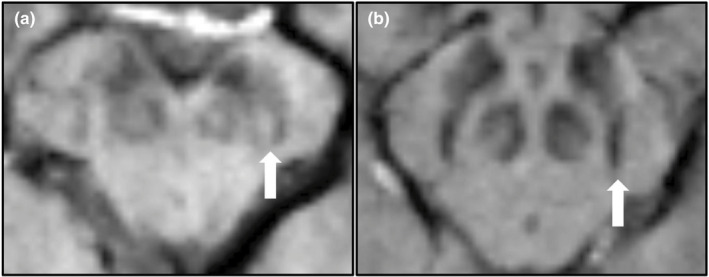
\includegraphics[width=0.8\linewidth]{FileAusiliari/Immagini/degenerative/BRB3-11-e02202-g002}
	\caption{Esempi di segno della coda di rondine (STS) in un individuo malato (a) e di STS assente in un individuo sano (b). Sono mostrate sezioni assiali del mesencefalo mappate tramite imaging pesato con suscettibilità (SWI). Le frecce bianche indicano la diversa configurazione del Nigrosoma-1 (N1). Da Brain Behav. 2021 May 24;11(7):e02202. doi: 10.1002/brb3.2202}
	\label{fig:brb3-11-e02202-g002}
\end{figure*}


La diagnosi differenziale delle sindromi parkinsoniane atipiche beneficia significativamente dell'imaging RM. L'atrofia multisistemica (MSA) evidenzia caratteristica atrofia putaminale, pontica e cerebellare, con ipointensità putaminale T2/SWI e "hot cross bun sign" pontino. La paralisi sopranucleare progressiva (PSP) manifesta atrofia mesencefalica con alterazione del rapporto mesencefalo-ponte, mentre la degenerazione corticobasale (CBD) presenta atrofia frontoparietale asimmetrica con iperintensità della sostanza bianca subcorticale.
Metodiche avanzate quali Diffusion Tensor Imaging (DTI) e risonanza magnetica funzionale (fMRI) consentono la caratterizzazione delle alterazioni microstrutturali della sostanza bianca e delle modificazioni funzionali cerebrali, sebbene la sensibilità nell'identificazione della progressione patologica e nella valutazione della risposta terapeutica necessiti ulteriore validazione. Le limitazioni metodologiche includono variabilità interindividuale e sovrapposizione dei reperti radiologici nelle diverse sindromi parkinsoniane.

\subsection{Trattamento e prognosi}

\subsection{Checklist di refertazione}

\begin{itemize}[label=$\square$] % Riquadro vuoto come simbolo
	\item Escludi altre cause di parkinsonismo (es ictus)
	\item Controlla il segnale dei nigrosomi
	\item Controlla il trofismo delle strutture sottotentoriali
\end{itemize}

\subsection{Bibliografia}
\small{
	
	
}

\note{Nota a margine}
\expl{Nota a margine colorata}
\section{Patologia}

\subsection{Definizione}

\subsection{Eziologia}

\subsection{Epidemiologia}

\subsection{Presentazione  clinica}

\subsection{Approccio diagnostico}

\subsection{Anatomia patologica}

\subsection{Imaging}

\subsection{Trattamento e prognosi}

\subsection{Checklist di refertazione}

\note{Nota a margine}
\expl{Nota a margine colorata}
%%% Parte 2

\newgeometry{top=35mm, bottom=35mm, left=15mm, right=15mm, headheight=0pt, headsep=0pt, marginparsep=0pt, marginparwidth=0pt, footskip=0pt, footnotesep=0pt}
\part*{\HUGE Neuroradiologia Pediatrica}\label{Parte2}
\restoregeometry

%%%CAPITOLI

\chapter{Mielinizzazione}


\chapter{Patologia cerebro-vascolare}
\minitoc
\section*{Lista abbreviazioni}

\section{Danno ipossico-ischemico}

\subsection{Definizione}
Il danno ipossico-ischemico pediatrico si riferisce a una combinazione di lesioni ipossiche e ipoperfusione al cervello fetale o neonatale. Questa condizione è una delle cause più comuni di paralisi cerebrale e altri gravi deficit neurologici nei bambini, con un'incidenza di 2-9 su 1000 nati vivi

\subsection{Eziologia}
L'ipossia-ischemia, una delle principali cause di encefalopatia neonatale, si verifica quando il flusso sanguigno al cervello è ridotto (ischemia) e l'ossigenazione del sangue è compromessa (ipossiemia). Questa condizione può portare a gravi conseguenze neurologiche e persino alla morte.

Le cause alla base del danno ipossico-ischemico sono varie, e possono essere raggruppate in base al momento in cui si verificano:

\begin{itemize}
	\tightlist
	\item
	\textbf{Fattori antepartum:} includono condizioni materne come ipotensione, trattamenti per l'infertilità, gravidanze multiple, infezioni prenatali e malattie della tiroide.
	\item
	\textbf{Fattori intrapartum:} si riferiscono a complicazioni durante il travaglio, come parto con forcipe, estrazione podalica, prolasso del cordone ombelicale, distacco della placenta, cordone ombelicale stretto attorno al collo e febbre materna.
	\item
	\textbf{Fattori postpartum:} comprendono complicanze che si manifestano dopo la nascita, come distress respiratorio grave, sepsi o shock.
\end{itemize}

Indipendentemente dalla causa specifica, i processi fisiopatologici sottostanti al danno ipossico-ischemico sono simili e includono una cascata di eventi:

\begin{itemize}
	\tightlist
	\item
	\textbf{Riduzione del flusso sanguigno cerebrale (ischemia):} porta a un passaggio dal metabolismo aerobico a quello anaerobico, causando una rapida deplezione di ATP e un accumulo di lattato nelle cellule.
	\item
	\textbf{Rilascio di neurotrasmettitori eccitatori:} come il glutammato, che attiva i recettori NMDA, provocando un afflusso di calcio nei neuroni postsinaptici.
	\item
	\textbf{Formazione di radicali liberi:} che danneggiano i costituenti cellulari, come i mitocondri, peggiorando la produzione di ATP e portando alla morte cellulare.
	\item
	\textbf{Edema citotossico:} causato dallo stress osmotico, con conseguente ridistribuzione dell'acqua dallo spazio extracellulare a quello intracellulare.
\end{itemize}
Inoltre, è importante considerare che la maturità del cervello neonatale al momento dell'insulto influisce sul tipo e sulla gravità del danno. Nei neonati pretermine, l'ipoperfusione porta a lesioni della sostanza bianca periventricolare, mentre nei neonati a termine, le lesioni si verificano principalmente nella sostanza bianca subcorticale e nella corteccia parasagittale. In caso di ipoperfusione grave, le aree vulnerabili includono il talamo e il tronco encefalico nei neonati pretermine e il talamo laterale, il putamen posteriore, l'ippocampo, il tronco encefalico e la corteccia sensomotoria nei neonati a termine.

\subsection{Epidemiologia}

L'encefalopatia ipossico-ischemica (HIE) è una delle principali cause di morbilità e mortalità neonatale, nonché di disabilità neurologiche a lungo termine.

\textbf{Epidemiologia}:

\begin{itemize}
	\tightlist
	\item
	L'HIE colpisce dall'1 al 6 ogni 1000 nati vivi. In particolare, nei paesi sviluppati, si stima un'incidenza di 1-3 casi ogni 1.000 nati vivi.
	\item
	Nei neonati a termine, l'HIE è responsabile del 15-20\% della mortalità neonatale.
	\item
	Nei neonati pretermine nati prima della 32esima settimana di gestazione, la mortalità può arrivare fino al 50\%.
	\item
	Circa il 50\% dei casi di paralisi cerebrale sono osservati in neonati prematuri.
	\item
	Nonostante un calo di mortalità perinatale e materna, l'incidenza di paralisi cerebrale non è cambiata negli ultimi 40 anni.
	\item
	Tra il 15\% e il 20\% dei neonati che soffrono di HII muoiono nel periodo neonatale e un ulteriore 25\% sviluppa deficit neurologici permanenti.
\end{itemize}

\subsection{Presentazione clinica}

La presentazione clinica del danno ipossico-ischemico (HII) nei neonati può variare a seconda della gravità e della durata dell'insulto, nonché dell'età gestazionale del neonato al momento dell'evento. I segni e i sintomi possono essere aspecifici nelle prime ore di vita e tendono a evolvere nel corso dei giorni.

Ecco alcuni aspetti chiave della presentazione clinica:

\begin{itemize}
	\tightlist
	\item
	\textbf{Anamnesi perinatale}: Spesso si riscontra un evento stressante perinatale noto, come un parto complicato o difficile, che porta a sospettare un HII. I neonati possono nascere con grave acidemia metabolica o mista, che si manifesta con un basso pH nel sangue del cordone ombelicale (\textless7), bassi punteggi di Apgar (\textless3) a 0 e 5 minuti dopo la nascita.
	\item
	\textbf{Segni neurologici}:
	
	\begin{itemize}
		\tightlist
		\item
		\textbf{Depressione della coscienza}: I neonati possono mostrare un livello di coscienza depresso.
		\item
		\textbf{Ipotonia}: È frequente la presenza di ipotonia, soprattutto in caso di lesione delle regioni corticali.
		\item
		\textbf{Alterazioni del tono muscolare}: I neonati possono presentare ipotonia o ipertonia.
		\item
		\textbf{Riflessi vivaci}: In alcuni casi si possono osservare riflessi vivaci.
		\item
		\textbf{Convulsioni}: Le convulsioni sono comuni, verificandosi nel 50-70\% dei neonati asfittici e generalmente iniziano entro le prime 24 ore.
		\item
		\textbf{Apnea e respiro periodico}: Nei primi giorni dopo un grave insulto, i neonati possono presentare respiro periodico con apnea.
		\item
		\textbf{Alterazioni dello stato di vigilanza}: Si possono osservare ipereccitabilità o prolungata veglia.
	\end{itemize}
	\item
	\textbf{Anomalie autonomiche}: I neonati possono mostrare segni di disfunzione autonomica, come bradicardia o tachicardia.
	\item
	\textbf{Altri sintomi}: I neonati possono manifestare alterazioni metaboliche come ipoglicemia, ipocalcemia e squilibri idro-elettrolitici. Possono inoltre verificarsi alterazioni renali, cardiache, polmonari e intestinali.
	\item
	\textbf{Esami elettrofisiologici}: L'elettroencefalogramma (EEG) può risultare anomalo. Un EEG anomalo può essere utile per prevedere l'esito clinico, inclusa la probabilità di morte e gravi sequele neurologiche a lungo termine.
	\item
	\textbf{Variazioni temporali}: I sintomi possono comparire dopo un periodo iniziale in cui il neonato sembra relativamente normale.
\end{itemize}

\textbf{È importante sottolineare che:}

\begin{itemize}
	\tightlist
	\item
	La gravità della presentazione clinica è correlata all'estensione e alla gravità del danno cerebrale.
	\item
	L'ipotermia terapeutica, iniziata entro 6 ore dall'asfissia perinatale, può ridurre significativamente la mortalità e la morbilità, diminuendo l'incidenza di disabilità, paralisi cerebrale e ritardi dello sviluppo.
\end{itemize}

In sintesi, la presentazione clinica dell'HII può essere complessa e variabile. I neonati con sospetta HII richiedono un'attenta valutazione clinica e, spesso, esami di neuroimaging per confermare la diagnosi e determinarne la gravità.

\subsection{Approccio diagnostico}

\subsection{Anatomia patologica}

\subsection{Imaging}

\subsubsection{TC}

L'imaging tramite tomografia computerizzata (TC) ha un ruolo limitato nella valutazione dell'encefalopatia ipossico-ischemica (HIE) neonatale, soprattutto se confrontato con l'ecografia (US) e la risonanza magnetica (RM).
\textbf{Limiti nella visualizzazione del danno da HIE:} La TC è generalmente considerata \textbf{poco sensibile} nella valutazione dell'HIE neonatale. In particolare, la TC ha diverse limitazioni:

\begin{itemize}
	\tightlist
	\item
	\textbf{Difficoltà nel rilevare danni alla sostanza bianca:} La TC ha una bassa sensibilità nella rilevazione del danno alla sostanza bianca e della necrosi neuronale, che sono caratteristiche dell'HIE. La normale bassa attenuazione della sostanza bianca neonatale, dovuta all'elevato contenuto d'acqua, può mascherare l'edema o altri segni precoci di danno.
	\item
	\textbf{Difficoltà nel rilevare lesioni sottili:} La TC può non evidenziare lesioni sottili, come quelle che si manifestano nella fase acuta o subacuta dell'HIE.
	\item
	\textbf{Esposizione a radiazioni ionizzanti:} La TC espone il neonato a radiazioni ionizzanti, cosa che non avviene con l'ecografia o la RM. Questo è un fattore importante, specialmente nei neonati che sono più vulnerabili agli effetti delle radiazioni.
\end{itemize}

\subsubsection{RM}
Nelle immagini pesate in T1 ottenute in neonati sani a termine, un focus di iperintensità dovrebbe essere sempre visibile nel braccio posteriore della capsula interna e dovrebbe avere un'intensità di segnale relativamente più elevata rispetto al putamen posterolaterale. I talami ventrolaterali e i globi pallidi, in particolare negli aspetti mediali, dovrebbero avere un'intensità di segnale più elevata rispetto agli altri nuclei della sostanza grigia profonda. Nelle immagini pesate in T2  si dovrebbe sempre osservare un focus di ipointensità nel braccio posteriore delle capsule interne e nei talami ventrolaterali.

I pattern di danno ipossico-ischemico (HII) nel cervello neonatale variano significativamente a seconda dell'età gestazionale e della maturazione cerebrale al momento dell'insulto. La maturità del cervello influenza la sua vulnerabilità alle lesioni, determinando quali aree saranno maggiormente colpite. In generale, l'HII non colpisce tutte le aree cerebrali uniformemente, ma mostra una "vulnerabilità selettiva'', con alcune regioni più suscettibili al danno rispetto ad altre. I pattern di danno possono essere suddivisi in base all'età gestazionale del neonato:

\textbf{Neonati pretermine (meno di 36 settimane di gestazione)}:

\begin{itemize}
	\tightlist
	\item
	\textbf{Ipoperfusione lieve-moderata}: il danno si manifesta principalmente nella sostanza bianca periventricolare (PVL). Ciò è dovuto alla vascolarizzazione ventricolopeta del cervello immaturo, in cui i vasi sanguigni penetrano dalla superficie del cervello verso le regioni periventricolari. La PVL può evolvere con un quadro di necrosi, cavitazione e sviluppo di cisti, che con il tempo possono collassare con conseguente gliosi e riduzione del volume della sostanza bianca. La PVL si osserva più frequentemente in prossimità dei trigoni dei ventricoli laterali e dei forami di Monro.
	\item
	\textbf{Ipoperfusione grave}: le lesioni coinvolgono principalmente le strutture della sostanza grigia profonda, come il talamo e il tronco encefalico. In particolare, il talamo, il verme anteriore del cervelletto e il tronco encefalico dorsale sono le aree più frequentemente colpite. È stato osservato che, nei neonati nati prima delle 32 settimane, il coinvolgimento dei gangli basali è meno grave rispetto al talamo. I gangli basali tendono a cavitare e ridursi senza cicatrizzazione. In questi casi si possono osservare anche emorragie della matrice germinale.
\end{itemize}

\textbf{Neonati a termine (36 settimane di gestazione o più)}:

\begin{itemize}
	\tightlist
	\item
	\textbf{Ipoperfusione lieve-moderata}: si osserva un pattern di danno ``periferico'' o ``a spartiacque'' (watershed). Le lesioni interessano principalmente la corteccia cerebrale e la sostanza bianca sottocorticale nelle zone di confine tra i territori vascolari delle arterie cerebrali anteriore, media e posteriore. Queste zone sono più vulnerabili a causa della ridistribuzione del flusso sanguigno a favore delle aree metabolicamente più attive.
	\item
	\textbf{Ipoperfusione grave}: il pattern di danno è definito ``dei gangli basali-talamo''. Questo tipo di danno è associato ad eventi ipossici o ischemici più gravi e di breve durata. Le aree più colpite sono il talamo laterale, il putamen posteriore, l'ippocampo, i tratti cortico-spinali e la corteccia sensomotoria. Inoltre, si può osservare una perdita del normale segnale iperintenso nella branca posteriore della capsula interna sulle immagini T1-pesate (segno della branca posteriore assente).
\end{itemize}

\textbf{Fattori che influenzano il pattern di danno}:

\begin{itemize}
	\tightlist
	\item
	\textbf{Maturità cerebrale:} La maturità del cervello al momento dell'insulto è uno dei principali fattori che determinano il pattern di danno. Il cervello pretermine è più vulnerabile alla PVL a causa della predominanza di pre-oligodendrociti, mentre il cervello a termine è più suscettibile al danno corticale e sottocorticale. Le aree con maggiore mielinizzazione e attività metabolica tendono ad essere più vulnerabili al danno.
	\item
	\textbf{Gravità dell'insulto:} episodi di ipossia-ischemia grave tendono a causare modelli di lesione più diffusi, con coinvolgimento delle strutture della sostanza grigia profonda. In particolare, nei neonati pretermine, un insulto grave può coinvolgere il talamo, il tronco cerebrale e il cervelletto, mentre nei neonati a termine un insulto severo coinvolge il talamo laterale, il putamen posteriore, l'ippocampo e la corteccia sensomotoria. Insulti meno severi interessano maggiormente la sostanza bianca periventricolare nei pretermine e le aree di spartiacque nei neonati a termine.
	\item
	\textbf{Durata dell'insulto:} insulti di breve durata spesso non causano danni cerebrali, mentre eventi prolungati portano a lesioni più estese.
\end{itemize}

Inoltre, i modelli di lesione possono essere influenzati dai meccanismi di ridistribuzione del flusso ematico cerebrale. In caso di ipossia, il flusso sanguigno viene reindirizzato verso le aree più vitali e metabolicamente attive come il tronco cerebrale e il talamo, a scapito di altre aree.

Le lesioni in HII possono evolvere nel tempo. Nella fase acuta, le lesioni possono essere caratterizzate da edema e restrizione della diffusione all'imaging DWI. Con il passare del tempo, può verificarsi un danno cellulare, con gliosi, atrofia e deposizione di minerali.

Gli infarti venosi periventricolari sono secondari alla trombosi delle vene midollari che drenano il parenchima cerebrale periventricolare e sono solitamente identificati come lesioni triangolari unilaterali con emorragia interna sulle immagini coronali. I neonati prematuri con infarti venosi periventricolari che coinvolgono la regione peritrigonale con associata assenza di mielinizzazione negli arti posteriori della capsula interna hanno una maggiore probabilità di sviluppare emiplegia congenita.

SWI e T2*GE sono particolarmente utili nell'imaging del cervello neonatale per identificare microemorragie e per migliorare la valutazione del danno ipossico-ischemico (HII).

\begin{itemize}
	\tightlist
	\item
	\textbf{Microemorragie}: Le sequenze SWI sono in grado di identificare \textbf{microemorragie} sia nella sostanza grigia che nella sostanza bianca. Queste emorragie possono non essere evidenti con le sequenze RM convenzionali e possono fornire informazioni importanti sulla tempistica e sull'estensione del danno.
	\item
	\textbf{Emorragie della matrice germinale}: Sia le sequenze GRE che le SWI possono evidenziare \textbf{emorragie della matrice germinale}, che sono più frequenti nei neonati pretermine. Le SWI possono essere superiori nel rilevare la componente emorragica di tali lesioni. L'emorragia della matrice germinale può essere associata a emorragie intraventricolari e può complicare ulteriormente il decorso clinico del neonato.
	\item
	\textbf{Trombosi venosa}: Le sequenze GRE e SWI possono essere utili nell'identificare la \textbf{trombosi venosa durale}, condizione che può associarsi a ischemia e danno cerebrale. La trombosi venosa si manifesta tipicamente con assenza di flusso nei seni venosi e, a volte, con emorragie correlate.
	\item
	\textbf{Depositi di emosiderina}: In caso di emorragie pregresse, le sequenze GRE e SWI possono evidenziare la presenza di \textbf{depositi di emosiderina}, un prodotto di degradazione dell'emoglobina, che può persistere a lungo dopo l'evento emorragico. I depositi di emosiderina possono essere utili per datare l'evento emorragico.
	\item
	\textbf{Coinvolgimento cerebellare:} Le sequenze SWI sono utili nell'identificare il coinvolgimento cerebellare, che è un reperto che può essere presente in casi di emorragia della matrice germinativa.
\end{itemize}

Le sequenze GRE e SWI sono più sensibili nel rilevare emorragie rispetto alle sequenze T1 e T2 convenzionali perché sono in grado di evidenziare anche piccole quantità di prodotti ematici. Le emorragie appaiono come aree di ipointensità nelle immagini GRE e SWI.

La spettroscopia di risonanza magnetica (MRS) è una tecnica di imaging avanzata che fornisce informazioni sul metabolismo cerebrale e può essere uno strumento prezioso nella valutazione del danno ipossico-ischemico (HII). A differenza della risonanza magnetica (RM) convenzionale che si concentra sulle immagini strutturali, la MRS analizza i livelli di determinati metaboliti nel tessuto cerebrale, offrendo indicazioni sulla funzione cellulare e sul danno metabolico.

\begin{itemize}
	\tightlist
	\item
	\textbf{Rilevamento precoce del danno:} La MRS è particolarmente utile nelle prime 24 ore dopo un evento ipossico-ischemico, quando le tecniche di imaging convenzionali possono non mostrare anomalie significative. La MRS può rivelare cambiamenti metabolici, come l'aumento del lattato, anche quando l'imaging strutturale è normale.
	\item
	\textbf{Valutazione della gravità del danno}: La MRS può essere più sensibile rispetto alla RM convenzionale nel valutare la gravità del danno cerebrale nelle prime ore dopo l'insulto. L'entità delle alterazioni metaboliche riscontrate con la MRS può essere correlata alla severità della lesione.
	\item
	\textbf{Misurazione del lattato}: La MRS è in grado di rilevare l'aumento del lattato (Lac) nelle aree cerebrali colpite. Il lattato è un indicatore di metabolismo anaerobico, che si verifica quando il tessuto cerebrale non riceve sufficiente ossigeno. Un picco di lattato a 1,3 ppm (a 1,5 T) è un reperto tipico in caso di lesione ipossica-ischemica acuta.
	\item
	\textbf{Identificazione di altri metaboliti}: La MRS può identificare anche altri metaboliti che cambiano a seguito di danno ipossico-ischemico come glutammina-glutammato, e può mostrare una diminuzione di N-acetil-aspartato (NAA), un marker di integrità neuronale. In alcuni casi si possono identificare alterazioni specifiche di alcuni disturbi metabolici. Per esempio, un picco a 0,9 ppm è tipico della malattia delle urine a sciroppo d'acero, e un picco di glicina a 3,56 ppm può essere presente nell'iperglicinemia non chetotica.
	\item
	\textbf{Valutazione prognostica}: Le alterazioni metaboliche rilevate con la MRS, come l'aumento del lattato e la diminuzione del NAA, sono state correlate con gli esiti neuroevolutivi nei neonati con HII. La combinazione di MRS e di altri esami di imaging può essere utile per predire il decorso neurologico a breve termine.
	\item
	\textbf{Distinzione tra lesioni ipossiche e metaboliche:} La MRS può essere utile nella diagnosi differenziale, ad esempio tra HII e patologie metaboliche, permettendo di identificare pattern metabolici specifici di alcune malattie. In caso di sospetti disturbi metabolici, una sequenza MRS appropriata (ad esempio, con un tempo di eco breve, TE 30-35ms) può consentire l'identificazione di specifici picchi di metaboliti caratteristici di tale disturbo.
	\item
	\textbf{Limitazioni}:
	
	\begin{itemize}
		\tightlist
		\item
		La MRS richiede più tempo rispetto all'imaging RM convenzionale.
		\item
		La MRS può studiare solo regioni di interesse specifiche.
		\item
		Le alterazioni dei metaboliti possono evolvere rapidamente, per questo sono consigliabili studi ripetuti nel tempo.
		\item
		L'interpretazione dei risultati può essere influenzata dall'ipotermia terapeutica, che attualmente rappresenta il trattamento di elezione per questa patologia.
	\end{itemize}
\end{itemize}

\paragraph{DTI}

L'imaging con tensore di diffusione (DTI) è una tecnica avanzata di risonanza magnetica (RM) che ha un valore significativo nella valutazione del danno ipossico-ischemico (HIE) nei neonati. Il DTI fornisce informazioni dettagliate sulla microstruttura cerebrale che non sono rilevabili con le tecniche di RM convenzionali.

\begin{itemize}
	\item
	\textbf{Valutazione della microstruttura cerebrale:} La DTI quantifica il movimento delle molecole d'acqua nei tessuti cerebrali utilizzando modelli matematici, consentendo di caratterizzare le strutture anatomiche microscopiche. Questa tecnica fornisce \textbf{misure quantitative} come l'\textbf{anisotropia frazionaria (FA)} e la \textbf{diffusività media (MD)}, che sono sensibili ai cambiamenti cellulari e extracellulari causati dall'HIE. Le alterazioni di questi parametri possono indicare edema citotossico, edema vascolare, infiammazione, morte cellulare e degenerazione walleriana.
	\item
	\textbf{Rilevazione precoce del danno:} La DTI può rilevare alterazioni del tessuto cerebrale nelle \textbf{prime fasi dell'HIE}, quando le tecniche di RM convenzionali possono risultare normali o solo leggermente alterate. In particolare, la DTI è più sensibile rispetto alla RM convenzionale nel rilevare \textbf{lesioni acute e subacute}. Le alterazioni di FA e MD possono indicare lesioni precoci, permettendo un intervento tempestivo.
	\item
	\textbf{Predizione della prognosi:} La DTI è uno strumento potente per \textbf{predire la prognosi} dell'HIE neonatale. Studi hanno dimostrato che alterazioni delle misure di DTI in regioni specifiche come il corpo calloso, il talamo, i gangli della base, il tratto corticospinale e la sostanza bianca frontale sono altamente predittive di esiti neurologici gravi.
	\item
	\textbf{Correlazione con la gravità del danno:} La DTI è utile per quantificare l'entità del danno cerebrale e per differenziare tra \textbf{HIE lieve, moderata e grave}. In generale, i casi di HIE grave sono associati a cambiamenti più estesi e severi nei valori di FA e MD rispetto ai casi lievi o moderati. \textbf{La gravità dei cambiamenti di FA e MD si correla con la gravità del danno cerebrale e della prognosi}.
	
	\begin{itemize}
		\tightlist
		\item
		Ad esempio, una riduzione di FA è stata osservata nei casi di HIE moderata-grave nelle prime 3 settimane di vita, mentre una riduzione della MD si osserva nella sostanza bianca nei casi più gravi.
		\item
		Valori bassi di FA nel tratto corticospinale e nel peduncolo cerebrale, e bassi valori di ADC nel tratto corticospinale e nei gangli della base sono stati correlati con una prognosi neurologica sfavorevole.
		\item
		Al contrario, elevati valori di ADC nella parte posteriore del braccio della capsula interna, si correlano con una migliore sopravvivenza e prognosi a due anni nei neonati con HIE.
	\end{itemize}
	\item
	\textbf{Monitoraggio dell'evoluzione del danno:} La DTI può essere utilizzata per monitorare l'evoluzione del danno nel tempo. È stato osservato che i valori di ADC tendono ad aumentare nella fase cronica, mentre i valori di FA diminuiscono. Le alterazioni di DTI cambiano nel tempo e possono differire a seconda della gravità e della tempistica dell'esame.
	\item
	\textbf{Identificazione di aree cerebrali specifiche coinvolte:} La DTI permette di identificare le aree cerebrali specifiche che sono state danneggiate dall'HIE. L'analisi basata su regioni di interesse (ROI) e le analisi basate su dati (come l'analisi voxel-by-voxel utilizzando la statistica spaziale basata sul tratto (TBSS) e i metodi basati su atlante (ABA) consentono di quantificare i valori di DTI per ogni regione anatomica. Studi hanno dimostrato che diverse regioni cerebrali sono coinvolte in modo differenziale nell'HIE.
	
	\begin{itemize}
		\tightlist
		\item
		Riduzioni di MD sono state osservate nel putamen, talamo, braccio anteriore e posteriore della capsula interna, sostanza bianca occipitale e tratto corticospinale.
	\end{itemize}
	\item
	Riduzioni di FA sono state osservate nel cervelletto in casi di HIE grave, insieme alla riduzione di MD nel peduncolo cerebellare superiore e riduzione di FA nel peduncolo cerebellare medio. * Aumenti di ADC accompagnati da riduzioni di FA sono stati osservati nei gangli della base, talamo, parte posteriore della capsula interna, peduncolo cerebrale e sostanza bianca periferica.
	\item
	\textbf{Studio della mielinizzazione:} La DTI è sensibile ai cambiamenti nella mielinizzazione della sostanza bianca. L'evoluzione dei parametri di DTI può fornire informazioni sullo sviluppo normale e patologico della mielina nei neonati con HIE. La DTI è in grado di studiare la traiettoria di sviluppo normale del cervello.
	\item
	\textbf{Approcci di analisi:}
	
	\begin{itemize}
		\tightlist
		\item
		\textbf{Analisi basata su ROI:} Prevede la selezione di regioni specifiche del cervello, con l'obiettivo di quantificare la DTI per queste regioni.
		\item
		\textbf{TBSS:} È un metodo per quantificare i valori scalari su base voxel per intere regioni della sostanza bianca, basato sulla scheletrizzazione delle mappe FA.
		\item
		\textbf{ABA:} Utilizza atlanti cerebrali per la quantificazione dell'immagine.
	\end{itemize}
	\item
	\textbf{Prognosi a lungo termine:} La DTI può fornire una predizione degli esiti neurologici a lungo termine, come le disabilità motorie e cognitive. Studi hanno dimostrato che alterazioni di FA e MD si correlano con esiti negativi nel neurosviluppo.
	\item
	\textbf{Limiti:} La DTI è sensibile alle differenze tra i tipi di scanner e i parametri di scansione, il che può rendere difficile il confronto tra studi diversi. Pertanto, è preferibile utilizzare un singolo scanner e un protocollo di scansione fisso negli studi scientifici.
\end{itemize}


\subsubsection{Ecografia}

L'ecografia transcranica (US) è uno strumento di screening potente e ampiamente disponibile per la valutazione dei neonati con sospetta encefalopatia ipossico-ischemica (HIE). Nonostante la risonanza magnetica (RM) sia considerata il "gold standard'' per l'imaging cerebrale neonatale, l'US ha diversi vantaggi che la rendono utile nella pratica clinica.

\begin{itemize}
	\item
	\textbf{Screening e diagnosi precoce:} L'ecografia è una tecnica \textbf{economica, portatile e facilmente accessibile}, che può essere eseguita al letto del paziente senza la necessità di sedazione. Questo la rende particolarmente utile per lo screening iniziale e la valutazione precoce dei neonati a rischio di HIE, soprattutto nei centri non accademici e nei paesi a basso reddito, o quando il paziente è troppo instabile per essere trasferito per una RM. L'US può identificare precocemente \textbf{segni di danno cerebrale} nei neonati con HIE, consentendo di iniziare tempestivamente le cure necessarie.
	\item
	\textbf{Valutazione del pattern e dell'estensione del danno:} L'US può contribuire a determinare il \textbf{pattern, il timing e l'estensione del danno} in caso di HIE. Questo è fondamentale per le implicazioni terapeutiche e per la previsione degli esiti neuroevolutivi. L'US può distinguere tra diversi tipi di lesioni, come l'\textbf{emorragia intraventricolare}, la \textbf{leucomalacia periventricolare} (PVL) e l'\textbf{infarto cerebrale}.
	\item
	\textbf{Monitoraggio nel tempo:} L'US può essere ripetuta nel tempo per definire l'\textbf{evoluzione delle lesioni} e per monitorare la risposta al trattamento. Studi ecografici seriali consentono di valutare la progressione o la regressione delle lesioni, così come la comparsa di eventuali complicanze come idrocefalo.
	\item
	\textbf{Valutazione dell'integrità vascolare:} L'ecografia Doppler può essere utilizzata per valutare le \textbf{dinamiche vascolari cerebrali} e l'\textbf{integrità dell'autoregolazione cerebrale}, tramite il calcolo dell'indice di resistenza (RI). Un RI anomalo (inferiore o uguale a 0.55) nelle prime 72 ore di vita è associato a una prognosi sfavorevole (morte o disabilità grave). L'indice resistivo diminuisce con l'aumentare dell'età gestazionale e deve essere correlato all'età gestazionale per ottenere risultati accurati. Tuttavia, il valore predittivo di un RI basso diminuisce durante l'ipotermia terapeutica e ritorna una volta che il neonato viene riscaldato.
	\item
	\textbf{Identificazione di lesioni specifiche:}
	
	\begin{itemize}
		\tightlist
		\item
		L'US può rilevare \textbf{aree di iperecogenicità} nella sostanza bianca periventricolare in caso di PVL. Nelle fasi iniziali della PVL (2-10 giorni di vita), si osserva una maggiore ecogenicità della sostanza bianca periventricolare, successivamente si possono formare delle cisti. Può essere presenta edema cerebrale e aspetto assottigliato dei ventricoli laterali.
		\item
		In caso di danno corticale, l'US può rivelare \textbf{regioni iperecogene a forma di cuneo} nelle zone di confine.
		\item
		L'US può essere utilizzata anche per lo screening di \textbf{emorragie intracraniche}.
	\end{itemize}
	\item
	\textbf{Limiti dell'ecografia:} Nonostante i suoi vantaggi, l'US presenta dei limiti rispetto alla RM. In particolare, \textbf{l'US ha una sensibilità inferiore rispetto alla RM} per la rilevazione di lesioni sottili, come le lesioni della sostanza bianca nel caso di danno ipossico-ischemico lieve o moderato e \textbf{non è in grado di visualizzare le strutture cerebrali con la stessa chiarezza} della RM. La RM è più accurata nell'individuazione di lesioni corticali e nel distinguere tra diversi pattern di danno.
\end{itemize}

\subsection{Trattamento e prognosi}

\subsubsection{Leucomalacia periventricolare}

La leucomalacia periventricolare (PVL) è una lesione della sostanza bianca cerebrale che si verifica comunemente nei neonati pretermine, ma può essere osservata anche nei neonati a termine. La patogenesi della PVL è complessa e multifattoriale, e coinvolge sia l'ischemia che la vulnerabilità delle cellule oligodendrogliali.

\begin{itemize}
	\tightlist
	\item
	\textbf{Vulnerabilità degli oligodendrociti:} La PVL è causata dalla \textbf{vulnerabilità selettiva} delle cellule della linea degli oligodendrociti a lesioni ipossiche-ischemiche. In particolare, i \textbf{preoligodendrociti}, precursori degli oligodendrociti maturi, sono particolarmente suscettibili ai danni da stress ossidativo e da eccitotossicità causati dall'ipossia. Questo è significativo perché, prima dell'inizio della mielinizzazione, la sostanza bianca è popolata principalmente da questi precursori. La PVL si manifesta più frequentemente nelle aree adiacenti ai trigoni dei ventricoli laterali e ai forami di Monro.
	\item
	\textbf{Ischemia:} In passato si credeva che la PVL fosse causata principalmente da \textbf{ischemia nelle zone di confine} della sostanza bianca periventricolare, in particolare nelle zone dove la vascolarizzazione è limitata. Si ipotizzava che la sostanza bianca nel cervello fetale immaturo fosse rifornita da arterie che penetravano dall'esterno verso i ventricoli, rendendo la sostanza bianca profonda più vulnerabile a diminuzioni della perfusione. Questa teoria è stata messa in discussione, tuttavia studi anatomici hanno evidenziato una bassa vascolarizzazione della sostanza bianca cerebrale fino a 32 settimane di gestazione, suggerendo un ruolo dell'ipovascolarizzazione nello sviluppo della PVL.
	\item
	\textbf{Eventi ipossico-ischemici:} Gli eventi ipossico-ischemici portano a una serie di eventi a cascata che contribuiscono allo sviluppo della PVL. Questi eventi causano un \textbf{danno alle cellule endoteliali} dei capillari della matrice germinativa, con conseguente perdita dell'integrità capillare. La riperfusione cerebrale successiva all'evento ipossico-ischemico può portare a \textbf{emorragie}, che possono essere rilevate con l'ecografia o la RM.
	\item
	\textbf{Infiammazione:} L'infezione o l'infiammazione possono peggiorare la PVL. Il rilascio di \textbf{citochine infiammatorie} può disturbare l'autoregolazione vascolare cerebrale, aumentando la suscettibilità al danno ipossico-ischemico.
\end{itemize}

\textbf{Evoluzione della PVL:}

\begin{itemize}
	\tightlist
	\item
	\textbf{Fase iniziale:} Inizialmente, si osserva \textbf{necrosi}, con aree di aumentata ecogenicità all'ecografia nelle regioni periventricolari entro le prime 48 ore.
	\item
	\textbf{Fase di normalizzazione:} Segue un periodo transitorio di relativa normalizzazione, generalmente dalla seconda alla quarta settimana di vita.
	\item
	\textbf{Formazione di cisti:} Successivamente, si sviluppano \textbf{cisti periventricolari} tra le 3 e le 6 settimane di vita. Queste cisti possono evolvere in pori encefalici.
	\item
	\textbf{Fase tardiva:} Con il tempo, le cisti si riducono e si sviluppa \textbf{gliosi}, con una significativa riduzione del volume della sostanza bianca nelle regioni periventricolari. La sostanza bianca periventricolare assume un aspetto iperintenso in T2 nelle immagini RM, e le pareti dei ventricoli possono apparire irregolari.
	\item
	\textbf{Stadio finale:} La fase finale della PVL è caratterizzata da \textbf{ventricolomegalia} con dilatazione dei trigoni, e un contorno irregolare dei ventricoli, con la perdita di volume della sostanza bianca periventricolare. Può esserci assottigliamento del corpo calloso, in particolare nella porzione posteriore e nello splenio.
\end{itemize}

\textbf{Reperti di imaging:}

\begin{itemize}
	\tightlist
	\item
	\textbf{Ecografia:} L'ecografia può rilevare inizialmente un'aumentata ecogenicità periventricolare, seguita dalla comparsa di cisti.
	\item
	\textbf{RM:} La RM consente una migliore visualizzazione delle anomalie della sostanza bianca periventricolare rispetto all'ecografia, specialmente quando ci sono aree non cistiche. La RM può evidenziare focolai di ipersignal T1, circondate da zone di ipersignal T2, che rappresentano l'astrogliosi reattiva e possibili depositi di mineralizzazione. La diffusione e la spettroscopia RM possono aiutare nella valutazione della lesione.
	\item
	\textbf{TC:} La TC non è utile nelle prime fasi della PVL, ma può essere utile per confermare i reperti di PVL allo stadio finale, come la riduzione di volume della sostanza bianca e la ventricolomegalia.
\end{itemize}

La gravità della PVL e l'estensione delle lesioni sono associate a un aumentato rischio di deficit neurologici a lungo termine, come la paralisi cerebrale. I deficit più comuni sono quelli motori e visivi, a causa del coinvolgimento delle vie motorie e visive che attraversano le regioni più colpite della sostanza bianca.

\subsection{Checklist di refertazione}

\subsection{Bibliografia}
\small{
	
	
}

\note{Nota a margine}
\expl{Nota a margine colorata}

\begin{itemize}[label=$\square$] % Riquadro vuoto come simbolo
	\item Primo elemento
	\item Secondo elemento
	\item Terzo elemento
\end{itemize}
\input{Capitoli/degenerative/approccio.tex}
\input{Capitoli/degenerative/degenerative.tex}
\section{Morbo di Parkinson}

\subsection{Definizione}

\subsection{Eziologia}

\begin{figure*}[h]
	\centering
	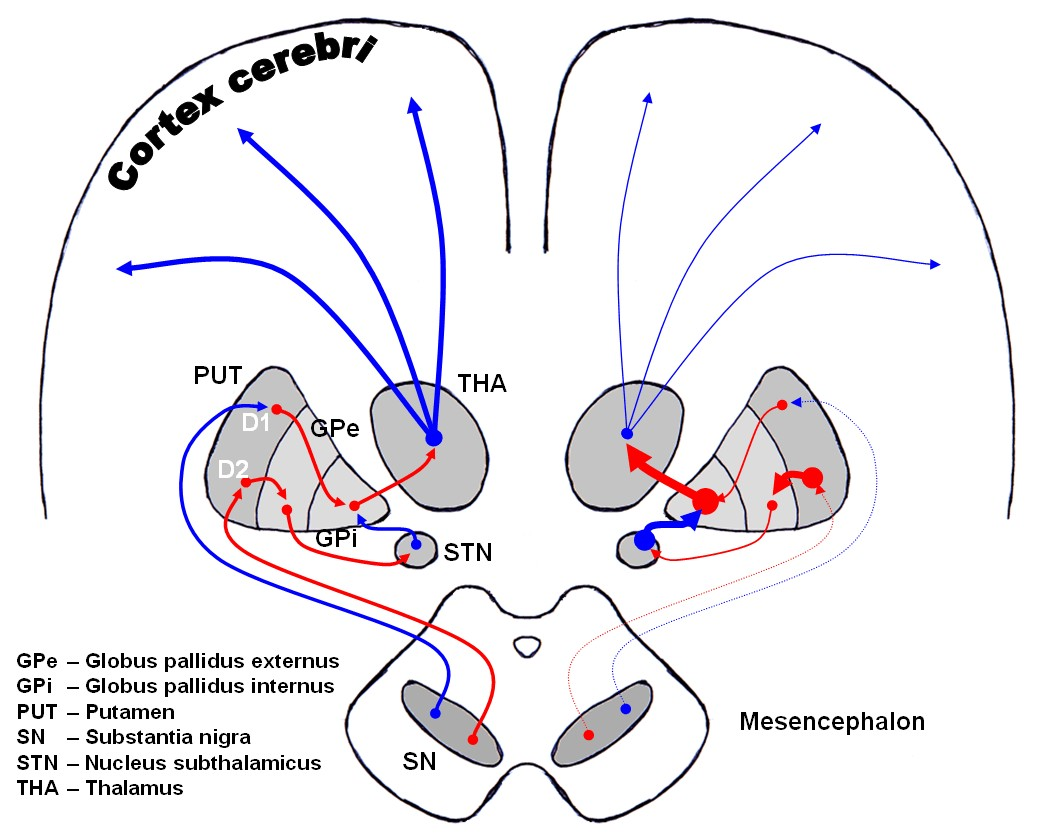
\includegraphics[width=0.5\linewidth]{FileAusiliari/Immagini/degenerative/dopamine-in-parkinsons-disease-illustration}
	\caption[Vie dopaminergiche]{L'immagine mostra le vie dopaminergiche del cervello umano in condizioni normali (a sinistra) e nella malattia di Parkinson (a destra). Le frecce rosse indicano la soppressione del bersaglio, quelle blu la stimolazione della struttura bersaglio. Caso per gentile concessione di Wikipedia, Radiopaedia.org, rID: 36286}
	\label{fig:dopamine-in-parkinsons-disease-illustration}
\end{figure*}

\subsection{Epidemiologia}
Il MP costituisce una delle principali cause di disabilità e mortalità nell'ambito delle patologie neurologiche, con una prevalenza particolarmente elevata negli Stati Uniti e in Canada (160-180 casi/100.000 abitanti). L'incidenza annuale in Nord America oscilla tra 108 e 212 casi ogni 100.000 individui di età $\geq$65 anni, con una prevalenza dello 0,3\% nella popolazione adulta $\geq$40 anni e dell'1,6\% nei soggetti ultrasessantacinquenni.
L'esordio della patologia mostra una significativa correlazione con l'età, manifestandosi tipicamente dalla quinta decade di vita, con un'età media alla diagnosi di 70,5 anni e una finestra di esordio prevalente tra i 45 e i 70 anni. Una variante giovanile può presentarsi tra i 20 e i 40 anni, sebbene l'esordio prima dei 30 anni risulti infrequente. La distribuzione per sesso evidenzia una predominanza maschile, particolarmente accentuata nella fascia d'età 50-60 anni.
L'eziologia del MP comprende fattori di rischio genetici, con particolare rilevanza nelle forme ad esordio precoce, e ambientali, tra cui l'esposizione a pesticidi e inquinanti atmosferici. Sono stati identificati fattori protettivi, inclusi il consumo di caffè, l'attività fisica e il fumo di sigaretta. La patologia si presenta prevalentemente in forma sporadica (85-90\% dei casi), mentre una minoranza dei casi (10-15\%) presenta familiarità positiva.

\subsubsection{Fattori di rischio}
L'eziopatogenesi del Morbo di Parkinson (MP) presenta una complessa interazione di fattori di rischio genetici, ambientali e non modificabili. L'anamnesi familiare positiva per MP in consanguinei di primo grado comporta un incremento del rischio relativo di 2-3 volte. Le forme monogeniche, rappresentanti meno del 10\% della casistica totale, manifestano pattern di ereditarietà autosomica dominante, recessiva o X-linked, caratterizzandosi per un esordio precoce rispetto alle forme sporadiche.
Le mutazioni eterozigoti del gene GBA1 costituiscono un significativo fattore di rischio genetico, unitamente ad alterazioni di altri geni codificanti per enzimi lisosomiali. Il coinvolgimento di geni quali SNCA, LRRK2, VPS35, Parkin, PINK1 e DJ-1 è stato ampiamente documentato. Particolare rilevanza assumono le mutazioni del gene Nurr1, determinante per l'identità neuronale dopaminergica, e del gene DJ-1, cruciale nella risposta allo stress ossidativo. Le alterazioni del gene PINK1, codificante per una chinasi mitocondriale, e del gene Park2, responsabile della sintesi della proteina parkina, sono associate a forme ad esordio precoce.
L'esposizione a neurotossine ambientali, inclusi mercurio, manganese, disolfuro di carbonio, solventi organici, MPTP e monossido di carbonio, può indurre degenerazione nigrostriatale e parkinsonismo. L'uso di neurolettici e l'abuso endovenoso di efedrone possono causare sindromi parkinsoniane potenzialmente irreversibili. Traumi cranici ripetuti, pesticidi, solventi e inquinamento atmosferico rappresentano ulteriori fattori di rischio ambientale documentati.
Tra i fattori non modificabili, l'età avanzata e il sesso maschile emergono come significativi predittori di rischio, con predominanza nella sesta decade di vita. Comorbidità quali depressione, ansia, stipsi, diabete mellito tipo 2, obesità e alterazioni del metabolismo del ferro sono state correlate a un incrementato rischio di MP.
Il consumo di tabacco e caffè, unitamente all'attività fisica regolare, ha mostrato effetti protettivi, sebbene di modesta entità. È fondamentale sottolineare che la maggioranza dei casi di MP rimane idiopatica, suggerendo un'eziologia multifattoriale.

\subsection{Presentazione  clinica}
La sintomatologia del Morbo di Parkinson manifesta un quadro clinico caratterizzato da manifestazioni motorie cardinali e sintomatologia non motoria associata. Il complesso sintomatologico motorio comprende tremore a riposo spesso asimmetrico con frequenza di 4-6 Hz, tipicamente descritto come "pill-rolling", bradicinesia manifestantesi con rallentamento motorio, ipomimia e ridotta oscillazione pendolare degli arti superiori durante la deambulazione, rigidità muscolare ("lead-pipe" o fenomeno della ruota dentata), e instabilità posturale documentabile attraverso il test della retropulsione. La deambulazione risulta caratterizzata da una progressione a piccoli passi con tendenza allo strascicamento e ridotta oscillazione degli arti superiori.
La sintomatologia accessoria include disartria con eloquio esplosivo secondario a incoordinazione linguo-diaframmatica, movimenti involontari della lingua con conseguente difficoltà protrusiva, e incremento della frequenza di ammiccamento palpebrale, quest'ultimo in contrasto con quanto osservato nella corea di Huntington. La disfunzione autonomica, i disturbi olfattivi, la sintomatologia algica, le alterazioni sensitive e i disturbi timici costituiscono il corredo sintomatologico non motorio. Il deterioramento cognitivo, con particolare coinvolgimento delle funzioni attentive, può manifestarsi e progredire nel decorso della patologia.
La progressione temporale della malattia evidenzia un esordio tipicamente unilaterale con successiva bilateralizzazione, manifestandosi prevalentemente nella sesta decade di vita. La responsività alla terapia dopaminergica, in particolare alla levodopa, rappresenta un elemento caratteristico, sebbene il tremore possa risultare farmacoresistente, in contrasto con la significativa risposta della bradicinesia e della rigidità. La variabilità fenotipica interindividuale costituisce un elemento distintivo della patologia.

\subsection{Approccio diagnostico}
L'iter diagnostico della malattia di Parkinson si fonda primariamente sulla valutazione clinica, data l'assenza di biomarcatori patognomonici. La diagnosi richiede la documentazione di bradicinesia associata ad almeno un sintomo cardine tra tremore a riposo o rigidità, valutati mediante la scala MDS-UPDRS standardizzata.
L'approccio diagnostico contempla un'accurata anamnesi ed esame obiettivo neurologico, focalizzati sull'identificazione dei sintomi cardinali: bradicinesia, tremore a riposo (4-6 Hz) tipicamente asimmetrico, rigidità e instabilità posturale. La responsività alla terapia dopaminergica, particolarmente evidente per bradicinesia e rigidità, costituisce un elemento diagnostico supportivo significativo, mentre una mancata risposta a dosaggi adeguati di levodopa suggerisce diagnosi alternative.
L'esclusione di parkinsonismi secondari richiede particolare attenzione all'insorgenza temporale dei sintomi e alla distribuzione topografica del coinvolgimento motorio. La diagnostica per immagini, sebbene non necessaria nelle presentazioni cliniche tipiche con adeguata risposta alla levodopa, può includere RM cerebrale, particolarmente utile mediante sequenze SWI per la valutazione del "swallow tail sign" nigrostriatale. La SPECT con 123I-FP-CIT (DaTscan) documenta la disfunzione dopaminergica presinaptica, mentre la PET con FDG consente la differenziazione metabolica tra PD e sindromi parkinsoniane atipiche.
L'analisi genetica, indicata in casi selezionati (esordio precoce, familiarità positiva, specifiche etnie), e la valutazione autonomica mediante scintigrafia miocardica con MIBG, che evidenzia la denervazione simpatica caratteristica, completano l'iter diagnostico. L'ecografia transcranica può evidenziare l'iperecogenicità della sostanza nera, supportando la diagnosi differenziale.
I criteri MDS stratificano la diagnosi in PD clinicamente stabilita e probabile, bilanciando specificità e sensibilità diagnostica nella pratica clinica.

\begin{Oss}
	La scala MDS-UPDRS (Movement Disorder Society-Unified Parkinson's Disease Rating Scale) è uno strumento di valutazione clinica ampiamente utilizzato per quantificare la gravità dei sintomi motori e non motori della malattia di Parkinson. Questa scala è stata sviluppata per migliorare la consistenza nella valutazione dei sintomi e per integrare meglio gli aspetti non motori della PD.
	Struttura: La scala MDS-UPDRS è composta da quattro sezioni:
	\begin{description}
		\item[Sezione I]{Esperienze non motorie della vita quotidiana. Questa sezione valuta aspetti come le capacità cognitive, i disturbi comportamentali e dell'umore}
		\item [Sezione II]{Esperienze motorie della vita quotidiana. Questa sezione valuta l'impatto dei sintomi motori sulle attività quotidiane}
		\item [Sezione III]{Esame motorio. Questa sezione valuta i segni motori della PD attraverso un esame clinico, come il tremore, la rigidità e la bradicinesia}
		\item[Sezione IV]{Complicanze della terapia. Questa sezione valuta le complicanze associate al trattamento farmacologico}
	\end{description}
	Il punteggio totale per le sezioni I-IV varia da 0 (nessuna disabilità) a 199 (disabilità totale). La sezione III, che valuta i sintomi motori, ha un punteggio che varia da 0 a 132.
	Oltre alla scala MDS-UPDRS, esistono altre scale di valutazione utilizzate nella PD, come la scala di Hoehn e Yahr e la scala di Schwab e England. La scala di Hoehn e Yahr valuta la gravità della malattia da 0 (nessuna malattia) a 5 (paziente costretto su sedia a rotelle o allettato senza assistenza).
\end{Oss}

\subsection{Anatomia patologica}
Dal punto di vista anatomopatologico il morbo di Parkinson si manifesta attraverso inclusioni proteiche intraneuronali denominate corpi di Lewy, costituiti primariamente da aggregati patologici di alfa-sinucleina, una proteina sinaptica fisiologicamente presente nel sistema nervoso centrale. L'accumulo di queste inclusioni, sebbene non patognomonico del morbo di Parkinson essendo documentabile anche nella demenza a corpi di Lewy, rappresenta una caratteristica istopatologica fondamentale quando localizzato nella substantia nigra, in associazione alla perdita neuronale dopaminergica. L'assenza di corpi di Lewy nelle forme post-encefalitiche, caratterizzate invece da grovigli neurofibrillari, e in alcune forme geneticamente determinate, sottolinea l'eterogeneità patogenetica della malattia.
La progressione spazio-temporale della patologia, codificata nello staging di Braak, delinea sei stadi evolutivi caratterizzati da una diffusione ascendente delle alterazioni neuropatologiche. Gli stadi iniziali (1-2) coinvolgono il nucleo motore dorsale dei nervi glossofaringeo e vago e il nucleo olfattivo anteriore, precedendo frequentemente la sintomatologia motoria. Gli stadi intermedi (3-4) documentano il coinvolgimento della substantia nigra pars compacta, del prosencefalo basale e della mesocorteccia temporale, correlando con l'esordio clinico della malattia. Gli stadi terminali (5-6) evidenziano una progressione neocorticale diffusa.
La patogenesi molecolare implica alterazioni del metabolismo dell'alfa-sinucleina, potenzialmente accelerate da disfunzioni delle proteine heat shock o dall'azione della dopamina. Il coinvolgimento della proteina parkin nella degradazione proteasomica evidenzia meccanismi neurodegenerativi potenzialmente indipendenti dalla formazione dei corpi di Lewy.
L'alfa-sinucleina, proteina fisiologicamente localizzata nelle terminazioni presinaptiche neuronali, manifesta nella patogenesi del morbo di Parkinson un processo patologico caratterizzato da misfolding proteico e successiva aggregazione in oligomeri, protofibrille e fibrille, culminante nella formazione dei corpi di Lewy intraneuronali. Questi aggregati proteici, considerati hallmark istopatologico della malattia, evidenziano particolare neurotossicità nella forma protofibrillare, determinando disfunzione e successiva degenerazione neuronale dopaminergica nigrostriatale.
L'identificazione di mutazioni nel gene SNCA, codificante per l'alfa-sinucleina, nelle forme familiari di malattia, unitamente alla documentazione di fenotipi clinici particolarmente aggressivi in presenza di duplicazione o triplicazione genica, ha fornito evidenze significative del ruolo causale di questa proteina nella patogenesi della malattia. La documentata capacità di trasmissione transcellulare dell'alfa-sinucleina patologica costituisce il substrato molecolare della progressione anatomopatologica descritta nello staging di Braak.
La disfunzione sinaptica correlata all'accumulo di alfa-sinucleina rappresenta un meccanismo patogenetico critico, modulato da fattori quali stress ossidativo, alterazioni del sistema ubiquitina-proteasoma e interazione con il metabolismo dopaminergico. Mutazioni nei geni parkin, PINK1 e DJ-1 influenzano il metabolismo dell'alfa-sinucleina attraverso alterazioni dei sistemi di degradazione proteica.
L'alfa-sinucleina costituisce attualmente un promettente target terapeutico, con particolare interesse per lo sviluppo di anticorpi monoclonali specifici e inibitori dell'aggregazione proteica, finalizzati al rallentamento della progressione patologica.

\subsection{Imaging}

\subsubsection{TC}
La TC manifesta un'utilità clinica circoscritta nella valutazione diagnostica primaria del MP, assumendo rilevanza nell'esclusione di patologie strutturali mimiche quali lesioni espansive, idrocefalo o alterazioni vascolari, particolarmente in presenza di presentazioni cliniche atipiche o "red flags" suggestive di diagnosi alternative.
Nel contesto della gestione terapeutica, la TC assume particolare rilevanza nella valutazione post-chirurgica della stimolazione cerebrale profonda (DBS), consentendo la verifica del corretto posizionamento degli elettrodi nel nucleo subtalamico (STN), tipicamente localizzati a 9mm dalla linea mediana, e l'identificazione di eventuali complicanze post-procedurali quali eventi emorragici, ischemici o fenomeni infiammatori transitori, questi ultimi caratterizzati da aree ipodense perilettrodiche a risoluzione graduale. L'utilità della metodica nel follow-up routinario post-DBS risulta secondaria.
La sensibilità subottimale della TC nella diagnosi differenziale tra PD e sindromi parkinsoniane atipiche, incluse atrofia multisistemica e paralisi sopranucleare progressiva, nonché nella distinzione dal tremore essenziale, ne limita significativamente l'applicazione clinica in questo contesto diagnostico.

\subsubsection{RM}
La RM è frequentemente normale nelle sequenze convenzionali (T1, T2, FLAIR) nelle fasi iniziali di malattia. L'implementazione di sequenze susceptibility-weighted imaging (SWI) o T2*-weighted ad alta risoluzione consente la visualizzazione del nigrosoma-1, struttura caratterizzata dal patognomonico "swallow tail sign", la cui perdita correla con la degenerazione dopaminergica nigrostriatale. L'accumulo patologico di ferro nella substantia nigra, quantificabile mediante sequenze SWI/T2* e incrementato del 50\% rispetto ai controlli, costituisce un ulteriore marker diagnostico, complementato dall'imaging della neuromelanina mediante sequenze T1 con impulsi di trasferimento di magnetizzazione (MTC).

\begin{figure*}[h]
	\centering
	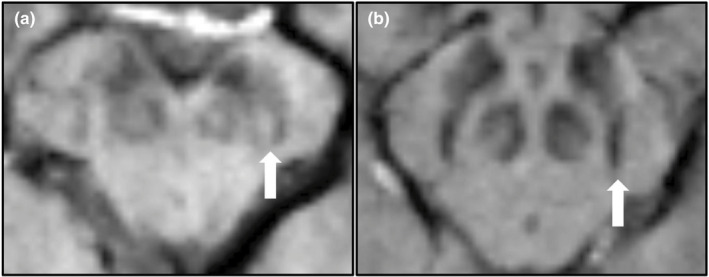
\includegraphics[width=0.8\linewidth]{FileAusiliari/Immagini/degenerative/BRB3-11-e02202-g002}
	\caption{Esempi di segno della coda di rondine (STS) in un individuo malato (a) e di STS assente in un individuo sano (b). Sono mostrate sezioni assiali del mesencefalo mappate tramite imaging pesato con suscettibilità (SWI). Le frecce bianche indicano la diversa configurazione del Nigrosoma-1 (N1). Da Brain Behav. 2021 May 24;11(7):e02202. doi: 10.1002/brb3.2202}
	\label{fig:brb3-11-e02202-g002}
\end{figure*}


La diagnosi differenziale delle sindromi parkinsoniane atipiche beneficia significativamente dell'imaging RM. L'atrofia multisistemica (MSA) evidenzia caratteristica atrofia putaminale, pontica e cerebellare, con ipointensità putaminale T2/SWI e "hot cross bun sign" pontino. La paralisi sopranucleare progressiva (PSP) manifesta atrofia mesencefalica con alterazione del rapporto mesencefalo-ponte, mentre la degenerazione corticobasale (CBD) presenta atrofia frontoparietale asimmetrica con iperintensità della sostanza bianca subcorticale.
Metodiche avanzate quali Diffusion Tensor Imaging (DTI) e risonanza magnetica funzionale (fMRI) consentono la caratterizzazione delle alterazioni microstrutturali della sostanza bianca e delle modificazioni funzionali cerebrali, sebbene la sensibilità nell'identificazione della progressione patologica e nella valutazione della risposta terapeutica necessiti ulteriore validazione. Le limitazioni metodologiche includono variabilità interindividuale e sovrapposizione dei reperti radiologici nelle diverse sindromi parkinsoniane.

\subsection{Trattamento e prognosi}

\subsection{Checklist di refertazione}

\begin{itemize}[label=$\square$] % Riquadro vuoto come simbolo
	\item Escludi altre cause di parkinsonismo (es ictus)
	\item Controlla il segnale dei nigrosomi
	\item Controlla il trofismo delle strutture sottotentoriali
\end{itemize}

\subsection{Bibliografia}
\small{
	
	
}

\note{Nota a margine}
\expl{Nota a margine colorata}

%%%%%								APPENDICI
\newgeometry{top=35mm, bottom=35mm, left=15mm, right=15mm, headheight=0pt, headsep=0pt, marginparsep=0pt, marginparwidth=0pt, footskip=0pt, footnotesep=0pt}
\part*{\HUGE Appendici}
\titleformat{\chapter}[display]    	{\bfseries\large\raggedright}    	{\vspace{-2.35cm} \MakeUppercase{\chaptertitlename}\ \Huge \thechapter}    	{.125ex}    	{\raggedleft\vspace{-1cm}\Huge\makebox[.5\textwidth]{}}
\titlespacing*{\chapter}{0pt}{6\baselineskip}{2.5\baselineskip}
\restoregeometry

	% Capitoli
\titlecontents{chapter}[2.5pc]
{\addvspace{15pt}}
{\begin{tikzpicture}
		\pgftext{\LArge\bfseries\bfseries\color{black}\hspace{-1cm} Appendice\ \thecontentslabel{\color{white}.}\hspace{.5cm} }
	\end{tikzpicture}\Large }
{}
{\color{black}\titlerule\; \;\Large\bfseries Pagina \thecontentspage}

\pagestyle{fancyapp}

\begin{appendices}
	\chapter{Titolo}\label{AppendiceA}
	\blindduck[maths]


%%%%%%%%%%%%%%%%%%%%%%%%%%%%									BACKMATTER
%%%%%%%%%%%%%%%%%%%%%%%%%%%%
\backmatter

%%%%% 							BIBLIOGRAFIA
\pagestyle{fancyBibliografia}
\titleformat{\chapter}
	[hang]
	{\vspace{-2cm}\Huge}
	{}
	{0em}
	{}
	[\Large {\begin{tikzpicture} [remember picture, overlay]
	\pgftext[right,x=14.75cm,y=0.2cm]{\HUGE\bfseries 
	Bibliografia}
	\end{tikzpicture}}]
	
	\nocite{*}
	\bibliographystyle{amsalpha}
	\bibliography{FileAusiliari/Bibliografia}
	\addcontentsline{toc}{part}{Bibliografia}
\cleardoublepage
%INDICE ANALITICO
 \pagestyle{fancyIndiceAnalitico}
 	\renewcommand{\indexname}{}
	% SISTEMA IL PROBLEMA DEL LINK ALL'INDICE ANALITICO
	\let\cleardoublepage\relax
	\titleformat{\chapter}[hang]{}{}{0em}{}[]
 	\chapter*{}
	\titleformat{\chapter}
		[hang]
		{\Huge}
		{}
		{0em}
		{}
		[\Large {\begin{tikzpicture} [remember picture, overlay]
		\pgftext[right,x=14.75cm,y=0.2cm]{\HUGE\bfseries 
			Indice analitico}
		\end{tikzpicture}}]
	\titlespacing*{\chapter}{0pt}{0\baselineskip}{5\baselineskip}
	\addcontentsline{toc}{part}{Indice analitico}	
	\vspace{-2cm}
	\printindex
%%%%%%%%%%%%%%%%%%%%%%%%%%%%%%%%%%%%%%%%%%%%%%%%%%%%%%%%%%%%%%%%%%%%%%%%%%%%%%%%%%%%%%%%%%%%%%%%%%%%%%%%%%%%%%%%%
\end{appendices}
\end{document}